%
%
% UCSD Doctoral Dissertation Template
% -----------------------------------
% http:\\ucsd-thesis.googlecode.com
%
%
% ----------------------------------------------------------------------
% WARNING: 
%
%  This template has not endorced by OGS or any other official entity.
%  The official formatting guide can be obtained from OGS.
%  It can be found on the web here:
%  http://ogs.ucsd.edu/AcademicAffairs/Documents/Dissertations_Theses_Formatting_Manual.pdf
%
%  No guaranty is made that this LaTeX class conforms to the official UCSD guidelines.
%  Make sure that you check the final document against the Formatting Manual.
%  
%  That being said, this class has been used successfully for publication of 
%  doctoral theses.  
%
%  The ucsd.cls class files are only valid for doctoral dissertations.
%
%
% ----------------------------------------------------------------------
% GETTING STARTED:
%
% Lots of information can be found on the project wiki:
% http://code.google.com/p/ucsd-thesis/wiki/GettingStarted
%
%
% To make a pdf from this template use the command:
%  pdflatex template
%
%
% To get started please read the comments in this template file 
% and make changes as appropriate.
%
%
% ----------------------------------------------------------------------
%
% A thesis using this template and class file was last successfully 
% submitted on 2009/03/19 (at least as far as I know).
%
% If you successfully submit a thesis with this package please let us
% know.
%
% ----------------------------------------------------------------------
% If you desire more control, please see the attached files:
%
%   * ucsd.cls    -- Class file
%   * uct10.clo   -- Configuration files for font sizes 10pt, 11pt, 12pt
%     uct11.clo                            
%     uct12.clo
%
% ----------------------------------------------------------------------



% Setup the documentclass 
% default options: 11pt, oneside, final
%
% fonts: 10pt, 11pt, 12pt -- are valid for UCSD dissertations.
% sides: oneside, twoside -- note that two-sided theses are not accepted 
%                            by OGS.
% mode: draft, final      -- draft mode switches to single spacing, 
%                            removes hyperlinks, and places a black box
%                            at every overfull hbox (check these before
%                            submission).
% chapterheads            -- Include this if you want your chapters to read:
%                              Chapter 1
%                              Title of Chapter
%
%                            instead of
%
%                              1 Title of Chapter
\def\RELEASE{}
\ifdefined\RELEASE
    \documentclass[12pt,chapterheads]{ucsd}
\else
    \documentclass[12pt,chapterheads,draft]{ucsd}
\fi


% Include all packages you need here.  
% Some standard options are suggested below.
%
% See the project wiki for information on how to use 
% these packages. Other useful packages are also listed there.
%
%   http://code.google.com/p/ucsd-thesis/wiki/GettingStarted



%% AMS PACKAGES - Chances are you will want some or all 
%    of these if writing a dissertation that includes equations.
%  \usepackage{amsmath, amscd, amssymb, amsthm}

%% GRAPHICX - This is the standard package for 
%    including graphics for latex/pdflatex.
\usepackage{graphicx}

\usepackage{booktabs}
\usepackage{tabularx}
\usepackage{array}
\newcolumntype{P}[1]{>{\centering\arraybackslash}p{#1}}
\newcolumntype{M}{>{\centering\arraybackslash} m{2cm} }

\usepackage{hyphenat} % allow for hyphenated words to be further hyphenated
                      % https://tex.stackexchange.com/a/2715
\usepackage{rotating}
\usepackage{multirow}
\usepackage{textcomp}
\usepackage{amssymb}
\usepackage{url}
\urlstyle{same}

%% SUBFIGURE - Use this to place multiple images in a
%    single figure.  Subfigure will handle placement and
%    proper captioning (e.g. Figure 1.2(a))
% \usepackage{subfigure}

%% LATIN MODERN FONTS (replacements for Computer Modern)
% \usepackage{lmodern}
% \usepackage[T1]{fontenc}


%% INDEX
%   Uncomment the following two lines to create an index: 
\usepackage{makeidx}
\makeindex
%   You will need to uncomment the \printindex line near the
%   bibliography to display the index.  Use the command
% \index{keyword} 
%   within the text to create an entry in the index for keyword.

%% HYPERLINKS
%   To create a PDF with hyperlinks, you need to include the hyperref package.
%   THIS HAS TO BE THE LAST PACKAGE INCLUDED!
%   Note that the options plainpages=false and pdfpagelabels exist
%   to fix indexing associated with having both (ii) and (2) as pages.
%   Also, all links must be black according to OGS.
%   See: http://www.tex.ac.uk/cgi-bin/texfaq2html?label=hyperdupdest
%   Note: This may not work correctly with all DVI viewers (i.e. Yap breaks).
%   NOTE: hyperref will NOT work in draft mode, as noted above.
 \usepackage[colorlinks=true, pdfstartview=FitV, 
             linkcolor=black, citecolor=black, 
             urlcolor=black, plainpages=false,
             pdfpagelabels]{hyperref}
% \hypersetup{ pdfauthor = {Your Name Here}, 
%              pdftitle = {The Title of The Dissertation}, 
%              pdfkeywords = {Keywords for Searching}, 
%              pdfcreator = {pdfLaTeX with hyperref package}, 
%              pdfproducer = {pdfLaTeX} }


\usepackage{verbatim}

\usepackage[toc,nopostdot,style=alttree]{glossaries}
\glssetwidest{PERMANOVAX}% widest name
\makeglossaries
\newacronym{mixs}{MIxS}{Minimum information about any (x) sequence}
\newacronym{ecg}{ECG}{Electrocardiograph}
\newacronym{ad}{AD}{Atopic Dermatitis}
\newacronym{emp}{EMP}{Earth Microbiome Project}
\newacronym{pcoa}{PCoA}{Principal Coordinates Analysis}
\newacronym{qiime}{QIIME}{Quantitative Insights into Microbial Ecology}
\newacronym{numpy}{NumPy}{Numerical Python}
\newacronym{pycogent}{PyCogent}{Comparative and Genomic Toolkit}
\newacronym{html5}{HTML5}{HyperText Markup Language, version 5}
\newacronym{webgl}{WebGL}{Web Graphics Library}
\newacronym{icomm}{ICoMM}{International Census of Marine Microbes}
\newacronym{king}{KiNG}{Kinemage, Next Generation}
\newacronym{hmp}{HMP}{Human Microbiome Project}
\newacronym{hgt}{HGT}{Horizontal Gene Transfer}
\newacronym{pca}{PCA}{Principal Component Analysis}
\newacronym{nmds}{NMDS}{Non-metric Multidimensional Scaling}
\newacronym{ca}{CA}{Correspondence Analysis}
\newacronym{fmt}{FMT}{Fecal Microbiota Transplant}
\newacronym{anosim}{ANOSIM}{Analysis of Similarities}
\newacronym{permanova}{PERMANOVA}{Permutational Multivariate Analysis of Variance}
\newacronym{ibd}{IBD}{Inflammatory Bowel Disease}
\newacronym{ena}{ENA}{European Nucleotide Archive}
\newacronym{cibdai}{CIBDAI}{clinical canine IBD activity index}
\newacronym{iqr}{IQR}{InterQuantile Range}
\newacronym{auc}{AUC}{Area Under the Curve}
\newacronym{otu}{OTU}{Operational Taxonomic Unit}
\newacronym{wsava}{WSAVA}{World Small Animal Veterinary Association}
\newacronym{bcs}{BCS}{Body condition scores}
\newacronym{dexa}{DEXA}{dual-energy X-ray absorptiometry}
\newacronym{gi}{GI}{Gastro Intestinal}
\newacronym{roc}{ROC}{Receiver operating characteristic}
\newacronym{sra}{SRA}{Sequence Read Archive}
\newacronym{cdi}{CDI}{\textit{Clostridium difficile} infection}
\newacronym{rcdi}{R-CDI}{recurrent \gls{cdi}}
\newacronym{nsaid}{NSAID}{Non-steroidal anti-inflammatory drug}
\newacronym{pcr}{PCR}{Polymerase Chain Reaction}
\newacronym{kegg}{KEGG}{Kyoto Encyclopedia of Genes and Genomes}
\newacronym{bmi}{BMI}{Body Mass Index}
\newacronym{cgr}{CGR}{Cardiac Glycoside Reductase}
\newacronym{t2d}{T2D}{type 2 diabetes}
\newacronym{irb}{IRB}{Institutional Review Board}
\newacronym{shime}{SHIME}{simulator of the human intestinal microbial ecosystem}
\newacronym{gnps}{GNPS}{Global Natural Products Social Molecular Networking}
\newacronym{ms}{MS}{Mass Spectrometry}
\newacronym{cd}{CD}{Crohn's disease}
\newacronym{uc}{UC}{Ulcerative Colitis}
\newacronym{icd}{ICD}{ileal CD}
\newacronym{hp}{HP}{healthy plane}
\newacronym{ccd}{CCD}{colonic Crohn's Disease}
\newacronym{gls}{GLS}{genetic load scores}
\newacronym{lc}{LC}{lymphocytic colitis}
\newacronym{cc}{CC}{collagenous colitis}
\newacronym{hc}{HC}{healthy controls}
\newacronym{glm}{GLM}{Generalized linear mixed effects model}
\newacronym{smp}{SMP}{Student Microbiome Project}
\newacronym{mp}{MP}{Moving Pictures}
\newacronym{snp}{SNP}{Single nucleotide polymorphism}
\newacronym{ucl}{UCL}{standard upper control limit}
\newacronym{md}{MD}{Microbial dysbiosis}
\newacronym{cdai}{CDAI}{Clinical Disease Activity Index}
\newacronym{biom}{BIOM}{Biological Observation Matrix}
\newacronym{json}{JSON}{JavaScript Object Notation}
\newacronym{hdf5}{HDF5}{Hierarchical Data Format version 5}


\begin{document}


%% FRONT MATTER
%
%  All of the front matter.
%  This includes the title, degree, dedication, vita, abstract, etc..
%
%
% UCSD Doctoral Dissertation Template
% -----------------------------------
% http:\\ucsd-thesis.googlecode.com
%
%


%% REQUIRED FIELDS -- Replace with the values appropriate to you

% No symbols, formulas, superscripts, or Greek letters are allowed
% in your title.
\title{Statistical Representations Of Microbial Systems}

\author{Yoshiki V\'azquez Baeza}
\degreeyear{2017}

% Master's Degree theses will NOT be formatted properly with this file.
\degreetitle{Doctor of Philosophy} 

\field{Computer Science}
\chair{Professor Rob Knight}
% Uncomment the next line iff you have a Co-Chair
% \cochair{Professor Cochair Semimaster} 
%
% Or, uncomment the next line iff you have two equal Co-Chairs.
%\cochairs{Professor Chair Masterish}{Professor Chair Masterish}

%  The rest of the committee members  must be alphabetized by last name.
\othermembers{
Professor Pieter Dorrestein\\
Professoe  Rachel Dutton\\
Professor  Jim Hollan\\
Professor Larry Smarr\\
}
\numberofmembers{5} % |chair| + |cochair| + |othermembers|


%% START THE FRONTMATTER
%
\begin{frontmatter}

%% TITLE PAGES
%
%  This command generates the title, copyright, and signature pages.
%
\makefrontmatter 

%% DEDICATION
%
%  You have three choices here:
%    1. Use the ``dedication'' environment. 
%       Put in the text you want, and everything will be formated for 
%       you. You'll get a perfectly respectable dedication page.
%   
%
%    2. Use the ``mydedication'' environment.  If you don't like the
%       formatting of option 1, use this environment and format things
%       however you wish.
%
%    3. If you don't want a dedication, it's not required.
%
%
\begin{dedication} 
	To my parents, my family and my friends.
\end{dedication}

% You are responsible for formatting here.
%\begin{mydedication} 
%  \vspace{1in}
%  \begin{flushleft}
%    To me.
%  \end{flushleft}
%   
%   \vspace{2in}
%   \begin{center}
%     And you.
%   \end{center}
%
%  \vspace{2in}
%  \begin{flushright}
%    Which equals us.
%  \end{flushright}
%\end{mydedication}



%% EPIGRAPH
%
%  The same choices that applied to the dedication apply here.
%

% The style file will position the text for you.
\begin{epigraph} 
  \emph{The purpose of computing is insight, not numbers}\\
  ---Richard Hamming
\end{epigraph}

%% SETUP THE TABLE OF CONTENTS
%
\tableofcontents

%%
%% This block was needed to re-format the title of the glossary to match the
%% headings of the list of figures and list of tables.
%%
%% start hack:
\renewcommand{\glossarysection}[2][]{
\newpage
\noindent
\centerline{LIST OF ABBREVIATIONS}
}
%% end hack

\printglossary[title=List of Abbreviations,toctitle=List of Abbreviations,nonumberlist ]
\listoffigures  % Uncomment if you have any figures
\listoftables   % Uncomment if you have any tables

%% ACKNOWLEDGEMENTS
%
%  While technically optional, you probably have someone to thank.
%  Also, a paragraph acknowledging all coauthors and publishers (if
%  you have any) is required in the acknowledgements page and as the
%  last paragraph of text at the end of each respective chapter. See
%  the OGS Formatting Manual for more information.
%
\begin{acknowledgements} 
 Thanks to whoever deserves credit for Blacks Beach, Porters Pub, and
 every coffee shop in San Diego. 

 Thanks also to hottubs.

    Section~\ref{section_review}, in full, is a reprint of the material as it 
    appears in ``Impacts of the human gut microbiome in therapeutics''. Y.  
    V\'azquez-Baeza, C. Callewaert, J. Debelius, E. Hyde, C.  Marotz, J. T.  
    Morton, A. Swafford, A. Vrbanac, P. C.  Dorrestein and R.  Knight.  
    \emph{Annual Reviews}. 58, 2017.

    Section~\ref{section_emperor}, in full, is a reprint of the material as it 
    appears in ``Emperor: a tool for visualizing high throughput microbial 
    community data''. Y. V\'azquez-Baeza, A. Gonzalez, M. Pirrung, R.  Knight.  
    \emph{GigaScience}, 2, 2013 The dissertation/thesis author was the primary 
    investigator and author of this paper. In addition, we thank Jackson Chen, 
    Jai Ram Rideout, Daniel McDonald, William Van Treuren, Jose Antonio 
    Navas\hyp{}Molina, Nickolas A. Bokulich, Adam Robbins\hyp{}Pianka and Greg 
    Caporaso for feedback and useful discussion regarding the design and 
    implementation of the software package. This work was supported in part by 
    the National Institutes of Health, the Crohns and Colitis Foundation of 
    America, the Alfred P. Sloan Foundation, and the Howard Hughes Medical 
    Institute. The dissertation/thesis author was the primary investigator and 
    author of this paper.

    Section~\ref{section_animations}, in full, is a reprint of the material as 
    it appears in ``Bringing the Dynamic Microbiome to Life with Animations''.  
    Y.  V\'azquez-Baeza, A. Gonzalez, L. Smarr, D.  McDonald, J.  T. Morton, J.  
    A.  Navas-Molina, R. Knight. \emph{Cell Host and Microbe}, 11, 2017. The 
    dissertation/thesis author was the primary investigator and author of this 
    paper.

    Section~\ref{dogs}, in full, is a reprint of the material as it appears in 
    ``Dog and human inflammatory bowel disease rely on overlapping yet distinct 
    dysbiosis networks''. Y. V\'azquez-Baeza, E. R. Hyde, J. S.  Suchodolski, 
    R. Knight.  \emph{Nature Microbiology}, 1, 2016. The dissertation/thesis 
    author was the primary investigator and author of this paper. We wish to 
    acknowledge the support provided by the Crohn's and Colitis Foundation of 
    American; the Templeton Foundation and the Keck Foundation (via the Earth 
    Microbiome Project), the National institutes of Health. We wish to thank 
    Zhenjiang Xu, Jon Sanders, Amnon Amir, Gail Ackermann, Jamie Morton, Luke 
    Ursell, Jessica Metcalf, Antonio Gonzalez and Emma Schwager for their 
    useful comments and feedback in the writing of this manuscript. 

    Section~\ref{section_plane}, in full, is a reprint of the material as it 
    appears in ``Dynamics of the human gut microbiome in inflammatory bowel 
    disease''.  J. Halfvarson, C. J. Brislawn, R. Lamendella, Y.  
    V\'azquez-Baeza, W. A. Walters, L. M. Bramer, M. D'Amato, F.  Bonfiglio, D.  
    McDonald, A. Gonzalez, E. E. McClure, M. F. Dunklebarger, R. Knight, J.  K.  
    Jansson. \emph{Nature Microbiology}, 2, 2017. The dissertation/thesis 
    author was the primary analyst and a co-author of this paper.

    Section~\ref{section_ibd}, in full, is a reprint of the material as it 
    appears in ``Guiding longitudinal sampling in inflammatory bowel diseases 
    cohorts''. Y. V\'azquez-Baeza, A. Gonzalez, Z. Zech Xu, A. Washburne, H.  
    Herfarth, R.  B.  Sartor, R. Knight. \emph{Gut}. 2017. The 
    dissertation/thesis author was the primary investigator and author of this 
    paper. We acknowledge grant support by NIH (P01-DK094779), the Crohn's and 
    Colitis Foundation, and the research coordinators of the UNC 
    Multidisciplinary IBD Center at UNC for patient recruitment. Additionally, 
    we thank Gail Ackermann, Jamie Morton and Justin Silverman for their 
    invaluable feedback and discussion provided in the preparation of this 
    manuscript.

    Section~\ref{section_moviefmt}, in full, is a reprint of the material as it 
    appears in ``Dynamic changes in short- and long-term bacterial composition 
    following fecal microbiota transplantation for recurrent Clostridium 
    difficile infection''.  A. Weingarden, A. Gonzalez, Y.  V\'azquez-Baeza, S.  
    Weiss, G.  Humphry, D. Berg-Lyons, D. Knights, T.  Unno, A. Bobr, J.  Kang, 
    A. Khoruts, R. Knight, M. J. Sadowsky. \emph{Microbiome}. 3, 2015.  The 
    dissertation/thesis author was a co-primary investigator and author of this 
    paper. This research was supported, in part, by NIH Grant R21AI091907 (to 
    AK and MJS). ARW was supported by a Doctoral Dissertation Fellowship from 
    the University of Minnesota Graduate School and by the Dennis W.  Watson 
    Fellowship in Microbiology. Work done in the Knight lab was funded by the 
    NIH, Crohn's \& Colitis Foundation of America, and the HHMI.  

    Section~\ref{section_fmt}, in full, is a reprint of the material as it 
    appears in ``Changes in microbial ecology after fecal microbiota 
    transplantation for recurrent C. difficile infection affected by underlying 
    inflammatory bowel disease''. S. Khanna, Y.  V\'azquez-Baeza, A.  Gonzalez, 
    S. Weiss, B.  Schmidt, D. A.  Muñiz-Pedrogo, J. F. Rainey 3rd, P. Kammer, 
    H. Nelson, M.  Sadowsky, A.  Khoruts, S. L. Farrugia, R. Knight, D. S.  
    Pardi, P. C.  Kashyap. \emph{Microbiome}. 5, 2017. The dissertation/thesis 
    author was the co-primary investigator and author of this paper.

\end{acknowledgements}


%% VITA
%
%  A brief vita is required in a doctoral thesis. See the OGS
%  Formatting Manual for more information.
%
\begin{vitapage}
\begin{vita}
  \item[2012] B.~S. in Biomedical Engineering, Universidad Iberoamericana, Ciudad de M\'exico
  \item[2016] M.~Sc. in Computer Science, University of California, San Diego
  \item[2017] Ph.~D. in Computer Science, University of California, San Diego 
\end{vita}


\begin{publications}

    \item \textsl{Author names marked with $\dagger$ indicate shared first co-authorship}.

    \item \textbf{Y. V\'azquez-Baeza}, A. Gonzalez, M. Pirrung, R. Knight. ``Emperor: a tool for visualizing high throughput microbial community data'', \emph{GigaScience}, 2, 2013.

    \item \textbf{Y. V\'azquez-Baeza}, A. Gonzalez, L. Smarr, D. McDonald, J. T. Morton, J. A. Navas-Molina, R. Knight. ``Bringing the Dynamic Microbiome to Life with Animations'', \emph{Cell Host and Microbe}, 11, 2017.

    \item \textbf{Y. V\'azquez-Baeza}, E. R. Hyde, J. S. Suchodolski, R. Knight. ``Dog and human inflammatory bowel disease rely on overlapping yet distinct dysbiosis networks'', \emph{Nature Microbiology}, 1, 2016.

    \item  $\dagger$S. Khanna, \textbf{$\dagger$Y. V\'azquez-Baeza}, A.  
        Gonzalez, S. Weiss, B. Schmidt, D. A. Muñiz-Pedrogo, J. F. Rainey 3rd, 
        P. Kammer, H. Nelson, M. Sadowsky, A. Khoruts, S. L. Farrugia, R.  
        Knight, D. S. Pardi, P. C. Kashyap. ``Changes in microbial ecology 
        after fecal microbiota transplantation for recurrent C. difficile 
        infection affected by underlying inflammatory bowel disease'', 
        \emph{Microbiome}. 5, 2017.

    \item J. Halfvarson, C. J. Brislawn, R. Lamendella, \textbf{Y. V\'azquez-Baeza}, W. A. Walters, L. M. Bramer, M. D'Amato, F. Bonfiglio, D. McDonald, A. Gonzalez, E. E. McClure, M. F. Dunklebarger, R. Knight, J. K. Jansson. ``Dynamics of the human gut microbiome in inflammatory bowel disease'', \emph{Nature Microbiology}, 2, 2017.
  
    \item $\dagger$A. Weingarden, A. Gonzalez, \textbf{$\dagger$Y.  
        V\'azquez-Baeza}, S. Weiss, G. Humphry, D. Berg-Lyons, D. Knights, T.  
        Unno, A. Bobr, J. Kang, A. Khoruts, R. Knight, M. J. Sadowsky.  
        ``Dynamic changes in short- and long-term bacterial composition 
        following fecal microbiota transplantation for recurrent Clostridium 
        difficile infection''. \emph{Microbiome}. 3, 2015.

    \item \textbf{Y. V\'azquez-Baeza}, C. Callewaert, J. Debelius, E. Hyde, C. Marotz, J. T. Morton, A. Swafford, A. Vrbanac, P. C. Dorrestein and R. Knight. ``Impacts of the human gut microbiome in therapeutics''. \emph{Annual Reviews}. 58, 2017.

    \item \textbf{Y. V\'azquez-Baeza}, A. Gonzalez, Z. Zech Xu, A. Washburne, 
        H. Herfarth, R. B. Sartor, R. Knight. ``Guiding longitudinal sampling 
        in inflammatory bowel diseases cohorts''. \emph{Gut}. 2017.

    \item \noindent\rule[0.5ex]{\linewidth}{0.5pt}

    \textsl{The following publications were not included as part of this dissertation, but were also significant byproducts of my doctoral training.}

    \item C. A. Lozupone, J. Stombaugh, A. Gonzalez, G. Ackermann, D. Wendel, \textbf{Y. V\'azquez-Baeza}, J. K. Jansson, J. I. Gordon, R. Knight. ``Meta-analyses of studies of the human microbiota''. \emph{Genome Research}. 23, 2013.

    \item J. A. Navas-Molina, J. M. Peralta-S\'anchez, A. Gonzalez, P. J.  
        McMurdie, \textbf{Y. V\'azquez-Baeza}, Z. Xu, L. K Ursell, C. Lauber, 
        H. Zhou, S. Jin Song, J. Huntley, G. L Ackermann, D. Berg-Lyons, S.  
        Holmes,. Gregory Caporaso, R. Knight. ``Advancing our understanding of 
        the human microbiome using QIIME''. \emph{Methods in enzymology}. 531, 
        2013.

    \item G. E Flores, G. Caporaso, J. B Henley, J. R. Rideout, D. Domogala, J. Chase, J. W Leff, \textbf{Y. V\'azquez-Baeza}, A. Gonzalez, R. Knight, R. R. Dunn, N. Fierer. ``Temporal variability is a personalized feature of the human microbiome''. \emph{Genome biology}. 15, 2014.

    \item S. Lax, D. P Smith, J. Hampton-Marcell, S. M Owens, K. M Handley, N. M Scott, S. M Gibbons, P. Larsen, B. D Shogan, S. Weiss, J. L Metcalf, L. K Ursell, \textbf{Y. V\'azquez-Baeza}, W. Van Treuren, N. A Hasan, M. K Gibson, R. Colwell, G. Dantas, R. Knight, J. A Gilbert. ``Longitudinal analysis of microbial interaction between humans and the indoor environment''. \emph{Science}. 345, 2014.

    \item D. Gevers, S. Kugathasan, L. A Denson, \textbf{Y. V\'azquez-Baeza}, 
        W. Van Treuren, B. Ren, E. Schwager, D. Knights, S. Jin Song, M.  
        Yassour, X. C Morgan, A. D Kostic, C. Luo, A. Gonzalez, D. McDonald, Y.  
        Haberman, T. Walters, S. Baker, J. Rosh, M. Stephens, M. Heyman, J.  
        Markowitz, R. Baldassano, A. Griffiths, F. Sylvester, D. Mack, S. Kim, 
        W. Crandall, J. Hyams, C. Huttenhower, R. Knight, R. J Xavier. ``The 
        treatment-naive microbiome in new-onset Crohn's disease''. \emph{Cell 
        Host \& Microbe}. 3, 2014.

    \item $\dagger$A. Gonzalez, \textbf{$\dagger$Y. V\'azquez-Baeza}, R.  
        Knight. ``SnapShot: the human microbiome''. \emph{Cell}. 158, 2014.

    \item $\dagger$A. Gonzalez, \textbf{$\dagger$Y. V\'azquez-Baeza},  J. B. Pettengill, A. Ottesen, D. McDonald, R. Knight. ``Avoiding Pandemic Fears in the Subway and Conquering the Platypus''. \emph{mSystems}. 1, 2016.

    \item R. A Quinn, J. A Navas-Molina, E. R Hyde, S. Jin Song, \textbf{Y. V\'azquez-Baeza}, G. Humphrey, J. Gaffney, J. J Minich, A. V Melnik, J. Herschend, J. DeReus, A. Durant, R. J Dutton, M. Khosroheidari, C. Green, R. da Silva, P. C Dorrestein, R. Knight ``From sample to Multi-Omics conclusions in under 48 Hours''. \emph{mSystems}. 1, 2016.

    \item J. W Debelius, \textbf{Y. V\'azquez-Baeza}, D. McDonald, Z. Xu, E. Wolfe, R. Knight. ``Turning participatory microbiome research into usable data: lessons from the American Gut Project''. \emph{Journal of microbiology \& biology education}. 1, 2016.

    \item J. Debelius, S. Jin Song, \textbf{Y. V\'azquez-Baeza}, Z. Zech Xu, A. Gonzalez, R. Knight. ``Tiny microbes, enormous impacts: what matters in gut microbiome studies?''. \emph{Genome Biology}. 17, 2017.

    \item J. T Morton, J. Sanders, R. A Quinn, D. McDonald, A. Gonzalez, \textbf{Y. V\'azquez-Baeza}, J. A Navas-Molina, S. Jin Song, J. L Metcalf, E. R Hyde, M. Lladser, P. C Dorrestein, R. Knight. ``Balance trees reveal microbial niche differentiation''. \emph{mSystems}. 2, 2017.

    \item S. Weiss, Z. Zech Xu, S. Peddada, A. Amir, K. Bittinger, A. Gonzalez, C. Lozupone, J. R. Zaneveld, \textbf{Y. V\'azquez-Baeza}, A. Birmingham, E. R Hyde, R. Knight ``Normalization and microbial differential abundance strategies depend upon data characteristics''. \emph{Microbiome}. 5, 2017.

    \item L. R. Thompson, J. G. Sanders, D. McDonald, A. Amir, J. Ladau, K. J.  
        Locey, R. J. Prill, A. Tripathi, S. M.  Gibbons, G. Ackermann, J. A.  
        Navas-Molina, S. Janssen, E. Kopylova, \textbf{Y. V\'azquez-Baeza}, A.  
        Gonzalez, J. T. Morton, S. Mirarab, Z. Z. Xu, L. Jiang, M. F.  Haroon, 
        J.  Kanbar, Q.  Zhu, S. Song, T. Kosciolek, N. A. Bokulich J. Lefler, 
        C. J.  Brislawn, G. Humphrey, S. M. Owens, J. Hampton-Marcell, D.  
        Berg-Lyons, V. McKenzie, N. Fierer, J. A. Fuhrman, A. Clauset, R. L.  
        Stevens, A.  Shade, K. S. Pollard, K. D. Goodwin, J. K. Jansson, J. A.  
        Gilbert, R.  Knight and The Earth Microbiome Project Consortium. ``A 
        communal catalogue reveals Earth’s multiscale microbial diversity''.
        \emph{Nature}. 2017.
\end{publications}

\end{vitapage}


%% ABSTRACT
%
%  Doctoral dissertation abstracts should not exceed 350 words. 
%   The abstract may continue to a second page if necessary.
%
\begin{abstract}

    Technological developments in the past thirty years, have transformed 
    sequencing\hyp{}based microbiology into a data-intensive field where 
    computing, and efficient representations are catalyzers of insight into 
    omnipresent and complex microbial interactions. Notably, classical 
    ecologists have set the foundations for the way we analyze these systems, 
    with some techniques dating back to the beginning of the twentieth century.  
    In this thesis, we expand and where possible reuse these techniques, to 
    unravel the hidden patterns comprising the human gut microbiome.

    To set an appropriate motivation and context to the rest of this work, 
    Chapter 1 reviews recent discoveries on the human microbiome and how 
    the communities within can be determinants on the action of therapeutic 
    agents. Next, in Chapter 2, we introduce EMPeror, an interactive analysis 
    and visualization tool that is crucial to the findings presented in later 
    chapters.

    The following three chapters study concrete examples where the microbiome
    has been implicated as a driver or marker for dysbiosis. Chapter 3
    describes how the microbial signature associated with \gls{cd} in humans,
    described in our previous work \cite{RN154}, is overlapping but distinct to
    that of dogs affected with \gls{ibd}. Surprisingly, unlike with humans, dog
    fecal samples alone are strong indicators of the disease. In Chapter 4, we
    study \gls{ibd} from a longitudinal perspective, revealing increased
    volatility in the gut microbiomes of subjects with \gls{ibd}, a property
    that does not appear to be present in unaffected controls. Furthermore, we
    use this as a predicting feature of the disease, and improve on the
    classification accuracy possible through a single fecal sample. In Chapter
    5, we study the effect of \glspl{fmt} to treat \glspl{cdi} and using the
    techniques described in Chapter 2, we show the first animated visualization
    of this process, a dramatic microbial transformation as the subjects
    recover from all \gls{cdi} symptoms. In addition, for \gls{cdi} patients
    who also suffer from a subtype of \gls{ibd}, a treatment with a \gls{fmt}
    results in an increased number of relapses and decreased microbial
    diversity.

    The closing chapter discusses these results and their possible
    applications, as well as future directions for computationally-centric
    microbiome research.

\end{abstract}


\end{frontmatter}



%% DISSERTATION

\chapter{The hidden world within ourselves}\label{chapter_review}

Recent years have seen an increased interest in the study of microbial
communities, partly driven by the affordability of the enabling technologies.
This new focus provides a previously ignored axis of understanding to a vast
number of research fields. In addition, this has uncovered a number of
associations and demonstrated mechanisms, where microbial communities are key
explanatory variables.

In fields where microbial communities were already taken into consideration,
these advancements allowed experiments to be conducted at an unprecedented
scale \cite{RN35, RN4061, RN4267}. As a consequence, the underlying software
and methods to analyze these studies needed to accommodate volumes of
information previously unseen. Notably, most of the software used in this
context has been developed to interpret and analyze interdisciplinary
experiments that span a broad range of seemingly disjoint fields (for example
biofuel development \cite{RN4268}, built environment \cite{RN4270, RN4083},
forensics \cite{RN4269, RN4271}, etc).  As such, we motivate the rest of the
work in this thesis by presenting a comprehensive survey focused on the human 
microbiome.  The following section appeared in the journal
\textsl{Annual Review of Pharmacology and Toxicology, 2017}.

\ifdefined\RELEASE
    \glsresetall

\chapter{Impacts of the human gut microbiome on therapeutics}

\section{Abstract}

The human microbiome contains a vast source of genetic and biochemical variation, and its impacts on therapeutic responses are just beginning to be understood. This expanded understanding is especially important because the human microbiome differs far more among different people than does the human genome, and it is also dramatically easier to change. Here we describe some of the major factors driving differences in the human microbiome among individuals and populations. We then describe some of the many ways in which gut microbes modify the action of specific chemotherapeutic agents, ranging from \glspl{nsaid} to cardiac glycosides, and outline the potential of \gls{fmt} as a therapeutic. Intriguingly, microbes also alter how hosts respond to therapeutic agents through various pathways acting at distal sites. Finally, we discuss some of the computational and practical issues surrounding use of the microbiome to stratify individuals for drug response, and envision a future where the microbiome will be modified to increase everyone’s potential to benefit from therapy.

\section{Introduction}

Although extensive work has linked the human genome to drug response, the idea that the microbiome, the collection of genes in our microbial symbionts, could affect drug response is much newer, with the majority of work conducted in the past ten years. This lack of attention is surprising. As far back as the 1970s, it was estimated that the number of microbial cells, mostly bacteria, associated with the human body was greater than the number of human cells carrying the human genome \cite{RN4045}. This observation has held to the present, albeit with narrowed error bars, leading to an estimate of 53\% microbial cells to 47\% human cells \cite{RN4039}. An important and more recent observation is that the unique microbial genes greatly outnumber the unique human genes, with estimates of the microbial genome catalog typically numbering into the millions \cite{RN4107,RN4041,RN4040} and dwarfing the ~20,000 or so human genes \cite{RN4043}. What role all these microbial genes play in drug metabolism, and what effect drugs in turn have on the microbiome, are just starting to be explored.

A key barrier was the inability to identify the specific types of organisms associated with each individual. Traditionally, the limiting factor was the use of culture-dependent approaches which enabled only a small percentage of microbial strains from the gut to be cultured. Newer techniques, such as the use of initially germ-free mice as a culture medium \cite{RN4044} and advances in microdrop culturing \cite{RN4046},  have greatly expanded this repertoire, but each system is still limited by the requirement for active growth. The ability to sequence DNA directly from the environment, pioneered by Pace and colleagues, revolutionized our view of the microbial world by eliminating the constraint of culture, with many studies focusing on the 16S rRNA gene as a universal taxonomic marker \cite{RN4047}. The first study applying culture-independent analysis on a large scale to the human gastrointestinal tract \cite{RN4048} revealed dramatic differences among individuals, and  sites in the distal large intestine. As in prior studies, stool served as a useful proxy for the intestinal contents (where most metabolism takes place) but failed to capture the diversity of any site perfectly \cite{RN4048}. Highly multiplexed assays with next-generation sequencing \cite{RN4056} allowed hundreds of microbiomes to be read out at once, dramatically decreasing the cost of assessing the microbiome. Further improvements in sequencing methodology \cite{RN4107, RN4041} and software techniques \cite{RN4052, RN4054, RN4053} dramatically expanded the accessibility of microbiome studies to a wide range of investigators, both at the marker gene level and at the shotgun metagenomic level \cite{RN4055}, where total DNA is extracted and all the genes analyzed.

Results from these studies re-conceptualized our view of the microbiome. For example, rather than a common core of shared organisms, different people have very different collections of microbes, even if they share a home and/or genetic material. Changes in the microbiome throughout the lifespan are dramatic, especially in early life, and are greater than microbiome differences among adult mammalian species. Such differences in different parts of the body are comparable to the differences among microbial communities in different physical environments, such as soil and water. These large differences in species and gene composition and their implications for drug metabolism are illuminated by studies that combine DNA sequencing with other methods, including metabolomics analyses.

Now that identifying the taxa in a given microbiome sample is routine, and identifying the gene repertoire increasingly accessible, one can link the individual diversity in gene content to drug metabolism and other gut-related associations (Figure~\ref{review_fig1}). However, a complicating factor, especially for case/control study designs, is the issue of causality: many drugs, ranging from the obvious (antibiotics) to the surprising (metformin), dramatically affect the microbiome, so separating cause and effect can be difficult. It is perhaps most useful to think of the microbiome as a dynamic system in which the microbiome affects how drugs are metabolized and these products of metabolism in turn change the microbiome, which then changes future responses even to the same pharmaceutical. Such dynamic systems thinking is common in ecology, and although many current microbiome research techniques stem from this discipline, its application remains relatively rare in medicine.

\begin{sidewaysfigure}[htbp]
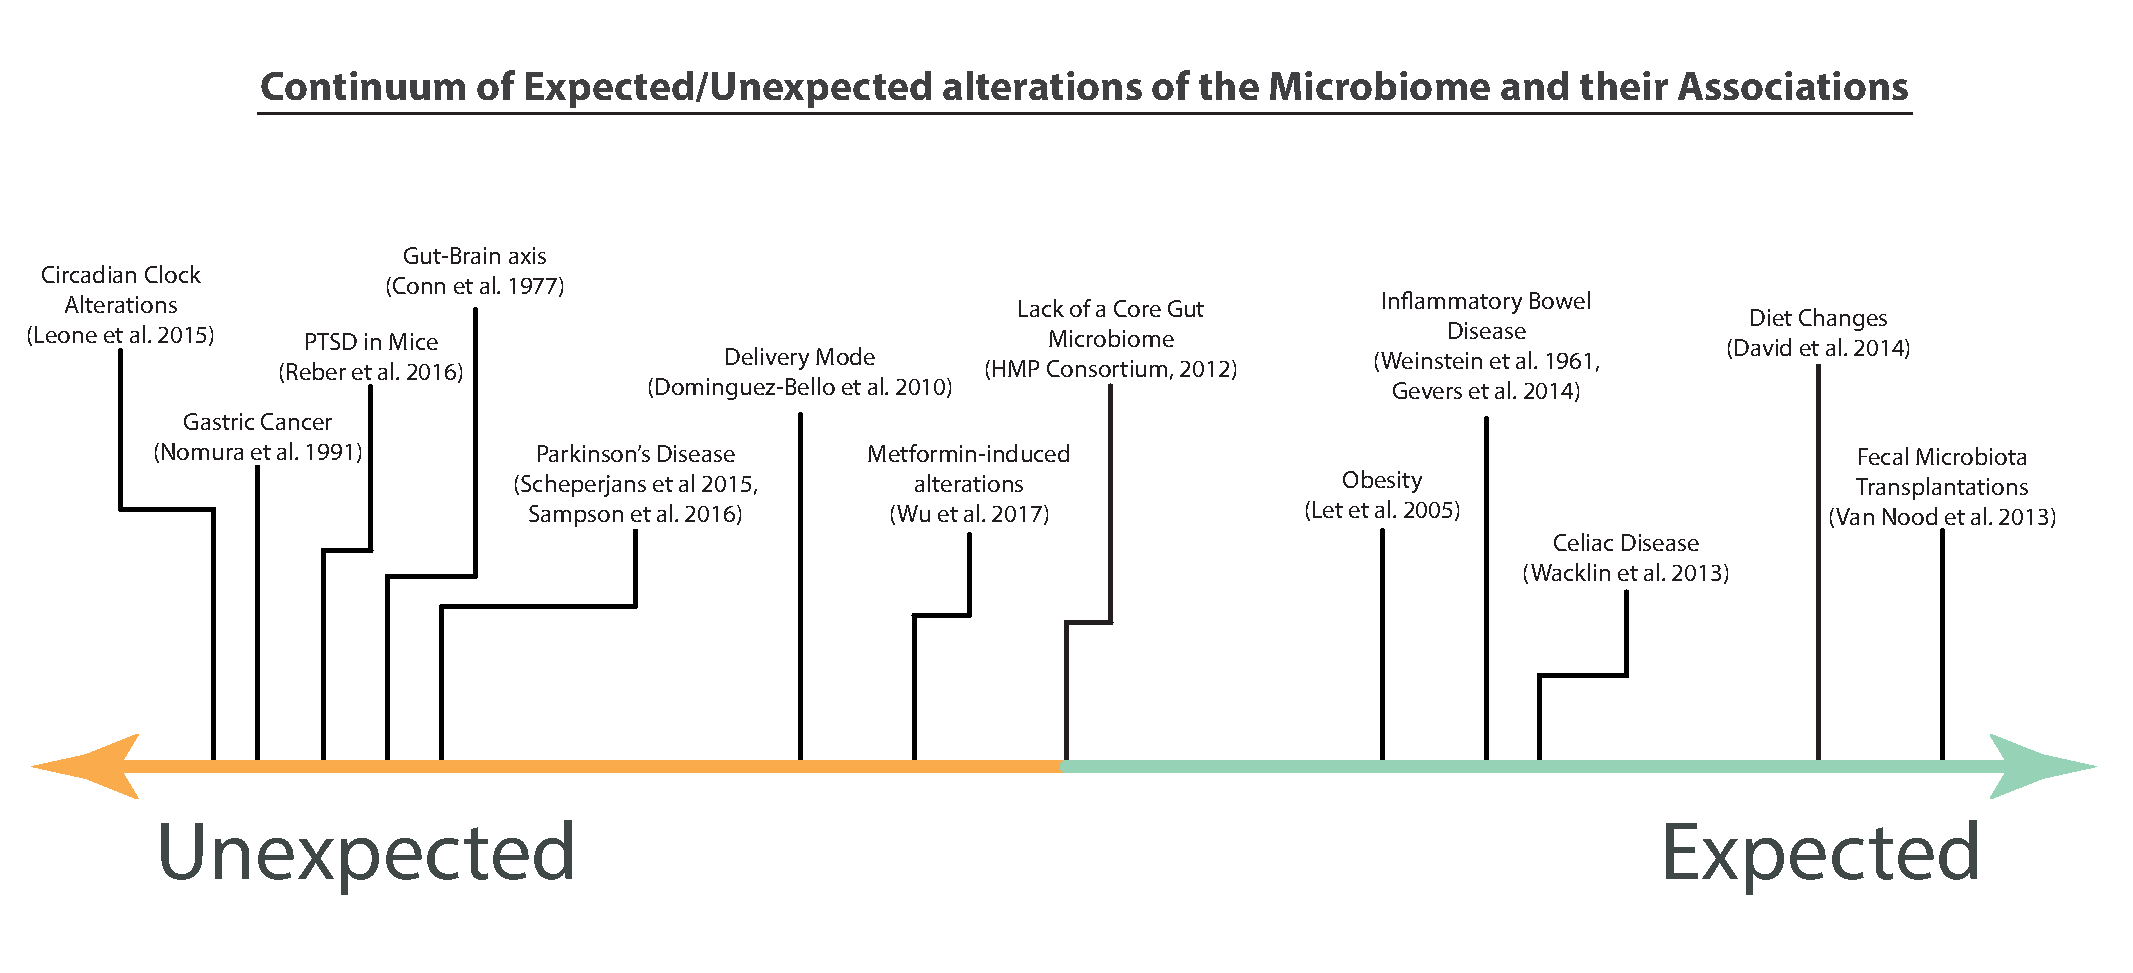
\includegraphics[width=0.95\textheight]{review-figures/figure-1}
\label{review_fig1}
\caption[A list of associations between the gut microbiome and various phenotypes]{A list of associations between the gut microbiome and various phenotypes, ranked by how expected or unexpected they were relative to previous knowledge [rank reflects consensus opinions of the co-authors of this Review, motivated by Figure 1 in \cite{RN4058}]}
\end{sidewaysfigure}


In this review, we focus on the human gut microbiome, although, where appropriate, we refer to studies using animal models, especially gnotobiotic mice (germ-free mice colonized with a defined set of microbes, either pure strains or fecal material from a rodent or human donor). As noted above, different parts of the human body (e.g., mouth, skin, airways, and urogenital tract) have distinct microbiomes from the gut microbiome, but the gut has been most studied in terms of drug response, in part because it contains by far the greatest microbial biomass in the human body, and therefore, the greatest capacity for drug metabolism. We first provide an overview of the diversity of the human gut microbiome, identifying key factors that structure the microbiome in healthy and diseased populations. We then describe connections between gut microbes and the action of several therapeutic agents, ranging from antibiotics to analgesics. Third, we describe how the microbiome can alter host response to drugs, though not necessarily metabolizing the drugs themselves. Fourth, we discuss prospects for identifying which patients will respond to a given drug based on the whole microbiome and prospects for exploiting the microbiome as a companion diagnostic to increase efficacy or reduce adverse events. Finally, we provide an outlook for the field in terms of improved patient stratification, and raise the intriguing prospect that patients might be converted from non-responders to responders via the use of companion therapies that alter the microbiome to increase efficacy of a specific drug.


\section{Diversity of the human gut microbiome across populations and life stages}

There are very few germ-free humans; therefore, understanding differences among individuals colonized with different microbes is key for predicting those who will respond similarly to drugs. However, many of the factors affecting the microbiome are highly counterintuitive. Here we focus primarily on a recent review \cite{RN4057}, five large-scale studies \cite{RN4108, RN4104, RN4107, RN4061, RN4059}, and two large-scale meta-analyses \cite{RN4062, RN4063} that summarize these findings.

As noted above, different sites in the human body host highly distinct microbial communities: on a Principal Coordinates Analysis `map' of the microbiome, they emerge as different `continents' \cite{RN4066, RN4107}. However, the differences in microbiome composition between, for example, the mouth and the gut of the same person are much greater than the differences between soil samples collected from different continents, and instead are more comparable to the difference between soil and seawater \cite{RN4087}. Although different body sites are highly distinct at the level of microbial taxa, they are relatively similar in terms of major microbial metabolic functions, at least as measured by \gls{kegg} pathways or other broad levels of gene function \cite{RN4107, RN4044}.

This pattern of microbial biogeography extends to the human gut \cite{RN4065, RN4066, RN4048, RN4070}. The microbiome changes dramatically along the gastrointestinal tract, with distinct populations in the oral cavity, esophagus, stomach, and small and large intestine. The most abundant genera of the oral cavity include \textit{Actinomyces}, \textit{Streptococcus}, \textit{Neisseria}, and \textit{Veillonella}, while the throat and stomach are dominated by \textit{Streptococcus} and \textit{Prevotella} species. In the stomach, roughly half of individuals are colonized by \textit{Helicobacteria pylori}, which dominates the gastric microbiome in these individuals \cite{RN4071}. The small intestine harbors fast-growing, G+C rich organisms specialized in digesting simple carbohydrates \cite{RN4067} and is often dominated by genera such as \textit{Peptostreptococcus}, which are rare in the large intestine. The bulk of the microbiome and microbial metabolism is in the large intestine. Typical bacterial loads are 105~CFU/ml in the jejunum, 106~CFU/ml in the ileum, but 108~CFU/ml in the cecum \cite{RN4110}, and 1011-1012~CFU/g in the feces \cite{RN4068}. This, together with stool being a relatively good proxy for the large intestine luminal contents but much more convenient to sample, means that most attention has focused on stool. However, for some applications such as detecting inflammatory bowel disease, microbiome analyses from biopsies dramatically outperform analyses of stool in their ability to distinguish healthy from diseased subjects \cite{RN4069}. The range of study designs where biopsies are essential is still hotly debated; nonetheless, stool biomarkers are highly informative for many applications, as noted below.

The process of development from infancy to early childhood has the greatest known effect on the stool microbiome. This effect is so profound that it traverses the vast gulf in microbiome configuration among body sites (Figure~\ref{review_fig2}). As they pass through the birth canal, newborns are typically colonized by bacteria resembling the constituents of the mother’s vaginal microbiome. By contrast, newborns delivered by C-section without labor lack these co-evolved vaginal microbes. Instead their microbiome resembles the skin, either from direct contact with caregivers and medical staff or from dust, which largely consists of human skin flakes and their associated microbes in indoor environments \cite{RN4115, RN4116, RN4118}. The first few weeks of life are chaos in the infant gut microbiome \cite{RN4120, RN4119} with very large differences at successive time points and among children. The subsequent overall process of development to the adult state takes about 2-3 years \cite{RN4115, RN4120, RN4061}, although smaller changes continue throughout childhood \cite{RN4061}. Intriguingly, although the process of development to the adult state is consistent cross-culturally, the state that is reached varies across populations \cite{RN4061}. These major differences in the microbiome may explain some of the differences in drug response between children and adults that are not explained by other factors.

\begin{figure}[htbp]
\includegraphics[height=0.65\textheight]{review-figures/figure-2}
\label{review_fig2}
\caption[Principal coordinates analysis on unweighted UniFrac distances of the process of microbiome assembly in the gut of one infant, contextualized with the Human Microbiome Project.]{Principal coordinates analysis on unweighted UniFrac distances of the process of microbiome assembly in the gut of one infant, contextualized with the Human Microbiome Project. Panel (A) colored by the sample type, and (B) colored by infant's age. As time goes by, the microbial communities in the infant's stool shift from resembling healthy adult vaginal and skin communities to resemble stool composition. This demonstrates how the process of gut microbiome development spans some of the most profound changes in the microbiome, i.e. the distance across different body sites.}
\end{figure}

Drugs that work in one human population may fail for unknown reasons in other populations, though the reasons for this are often obscure. Large efforts (and amounts of money) have sought the answer by studying human genomes. However, human genomes are 99.9\% the same but gut microbiomes can be 90\% different \cite{RN4081}. Given the rate of microbial metabolism and diversity of microbially-encoded enzymes, it makes sense to inquire whether  differences in drug responses are linked to the gut microbiome. Indeed, different human populations have markedly different microbiomes, which are largely thought to be linked to diet, with an axis that trades \textit{Prevotella} in diets rich in sugar and grains for \textit{Bacteroides} in diets rich in animal protein. These trends have been observed in the US population \cite{RN4088} and among US, South American, and African populations \cite{RN4061}. However, diet cannot be the sole driver, or between-population microbiome variation would not exceed the within-population variation, yet this is what one observes.

Even with hundreds of individuals, it is not yet possible to ascertain the factors at the population level that are most important in structuring the adult gut microbiome, because diet, environmental (including drug) exposures, host genetics, and other factors vary among populations in complex ways. Studies encompassing dozens of populations, with detailed tracking of individual- and population-level information, are likely required to resolve these questions, just as for such questions in human population genetics \cite{RN4078}. Hunter-gatherer populations, such as the Yanomami in the Amazon basin and the Hadza in sub-Saharan Africa, have distinct microbiomes harboring entire phyla, such as Spirochetes, that are even absent from rural farming populations \cite{RN4111, RN4113, RN4112}. This suggests that the loss of diversity from the microbiome of modern populations may have begun with the advent of agriculture. However, other factors such as C-section, antibiotics, and hygiene practices may be leading to continual depletion of our natural microbial symbionts \cite{RN4079}.

Several population-based studies that examine many variables have begun to provide insights into factors that shape microbiomes within populations. Drugs, especially antibiotics, but also metformin and proton pump inhibitors, have a surprisingly large effect on the microbiome and must be controlled for in studies that seek to link microbiomes to disease \cite{RN4080}. Long-term diet has a large effect, especially the balance of carbohydrates and protein. Age and season have large effects, although it is not known whether these are mediated in part by diet. Having a dog has an intermediate effect, smaller in the gut than in the skin and in the indoor environment \cite{RN4083, RN4082}. Many other factors, including sex, \gls{bmi}, and even amounts of sleep and exercise can be identified as differences among groups that contain hundreds of subjects per group but cannot be used to classify individuals. Host genetics has a surprisingly small impact in humans compared to other factors: although monozygotic twins are slightly more similar to one another than are dizygotic twins, hundreds of twin pairs are needed to see this effect. However, some specific components of the microbiome are highly heritable and correlate with phenotype. For example, Christensenella, identified by microbiome-wide heritability analysis, correlated with low \gls{bmi}, including in slimmed down germ-free mice that received an otherwise obesogenic microbiome from an obese human donor. Replicating this feat to manipulate weight or other phenotypes in humans remains a goal for future studies.

\section{Connections between specific gut microbes and action of therapeutic agents}
  
The literature demonstrating how gut microbes affect the efficacy or toxicity of specific drugs is expanding rapidly. Here we provide a few illustrative examples see also Table~\ref{review_tab1} for a brief summary. For additional examples, readers should  consult recent reviews \cite{RN4084,RN4086}.

\subsection{Analgesics}
\Glspl{nsaid} are used for pain relief in many conditions. Multiple studies have demonstrated that \gls{nsaid} use is associated with damage to the small intestine; the severity of this damage depends on the microbial community present at the time of \gls{nsaid} administration \cite{RN4107, RN4109}. Increased Gram-negative taxa have been associated with more severe damage \cite{RN4109, RN4124}. However, the precise link between \gls{nsaid}-induced damage and the microbiome remains poorly understood. Antibiotic treatment can alter the existing microbial community enough to reduce \gls{nsaid}-associated small intestinal damage in humans \cite{RN4085}, and can alter microbial metabolism of aspirin to potentiate its anti-thrombotic effects in mice \cite{RN4090}. However, other known negative effects of antibiotic treatment suggest risks in using antibiotics to reduce adverse events from specific combinations of microbiome state and \gls{nsaid} use. For example, antibiotic treatment of mice transplanted with a microbiome considered to be `protective' against \gls{nsaid} damage produced higher mortality with \gls{nsaid} administration \cite{RN4089}, underscoring that the association between \gls{nsaid} usage, microbiome community structure, and bowel damage reduction is complex and must be approached carefully. Probiotic strains have been deployed to prevent \gls{nsaid}-induced bowel damage. For example, protective effects of \textit{Lactobacillus gasseri} against aspirin-induced small intestinal damage have been assessed in human subjects \cite{RN4091}, and although results were promising, studies in larger populations are needed to evaluate the efficacy of this approach. In addition, the impact of the gut microbiome on the bioavailability, efficacy and toxicity of orally administered drugs, xenobiotics and dietary substances was studied for $>$30 pro-drugs \cite{RN4136}. Many prodrugs that treat gut inflammation are converted to active forms by the gut microbiome. These include sulfasalazine, olsalazine, ipsalazide and balsalazide, for which the aminosalicylic acid needs to be released in order to become active \cite{RN4093}. Gut bacteria of the genera Clostridia and Eubacteria exhibit this ability \cite{RN4094}.

\subsection{Antibiotics}
Although antibiotics influence the composition of the microbiome, the effects of antibiotic treatment depend on its starting composition. The extent of cellular damage induced by ex vivo antibiotic exposure of fecal samples depends on the individual's original microbiota \cite{RN4095}. This is consistent with previous data demonstrating species-specific susceptibility to antibiotics \cite{RN4096}. Healthy adults with similar microbial communities prior to treatment with cefprozil had similar alterations in the abundance of \textit{Enterobacter cloaceae} following treatment \cite{RN4097}. The gut microbiome may also regulate the effect of antibiotics at distal sites of infection. Resistance genes that lead to chemical modifications, such as hydrolysis or chemical modification, may decrease the bioavailability of the antibiotic \cite{RN4098}, potentially leading to a lower effective concentration at the primary site of infection. Future work is needed to investigate whether the overall gut microbiome composition influences these resistance genes.

\subsection{Cardiac glycosides}
Cardiac glycosides are a family of organic compounds that increase the contractility of the heart and are prescribed mainly for congestive heart failure and cardiac arrhythmia. The bioavailability of one of the most common cardiac glycosides, digoxin, varies greatly among patients. Early experiments showed that some patients’ gut microbiota can metabolize digoxin into inactive metabolites and that pretreatment with antibiotics in individuals harboring these microbiota increased the plasma level of digoxin \cite{RN4099}. Detailed metagenomic analysis identified a \gls{cgr} operon in some, but not other, strains of the commensal gut bacteria \textit{Eggerthella lenta}, which is responsible for the degradation of this drug \cite{RN4102}. Studies in animal models revealed that supplementation with the amino acid arginine can suppress the cgr operon and increase digoxin bioavailability. These experiments underline the importance of the microbiome in drug metabolism and provide an example where targeted therapeutic alternatives, in this case arginine supplementation in place of antibiotic treatment, can improve clinical outcomes.

\subsection{Metformin}
Metformin is used in the treatment of \gls{t2d}. Since its introduction in the 1950s \cite{RN4103}, many mechanisms of action have been proposed to explain its effects on the liver and insulin-sensitive tissues \cite{RN4126}. However, a recent report of trans-species transmission of the therapeutic effect of improved glucose tolerance from the stool of metformin-treated humans into germ-free mice \cite{RN4127} suggests that the insulin-sensitizing effects of the drug may result from a metabolic shift in the gut microbiome rather than direct effects on the liver or other tissues. Further evidence for this mechanism is suggested by the fact that most common side-effects of metformin are GI-centric (nausea, vomiting and diarrhea), and delivery of metformin into the portal vein did not change hepatic glucose production \cite{RN4128}.

\subsection{Fecal microbiota transplants (FMT)}
Microbiome transplants could potentially be used for many indications in the gut, but also in skin, oral, eye and vaginal health. The most prominent example is the treatment of recurrent \gls{cdi}. The standard of care for recurrent \gls{cdi} is antibiotics, which inadvertently deplete other microbes necessary for healthy gut function. \Gls{fmt} have outstanding efficacy in treating \glspl{cdi} \cite{RN4129}. The procedure relies on finding a healthy donor (often a close-relative or friend, although the evidentiary basis for this choice is weak), who donates fecal microbes for transplant into the diseased subject. Changes occur in the microbial communities of the recipient in less than a day, and disease-associated symptoms quickly disappear \cite{RN4130}. A meta-analysis of longitudinal datasets revealed that post-FMT subjects also recover dynamic features common to healthy humans \cite{RN4131}. \Glspl{fmt} are not 100\% effective and there is even anecdotal evidence of unintended changes, such as sudden excessive weight gain post-\gls{fmt} \cite{RN4132}. This has led researchers to seek optimal conditions for effective \gls{fmt}, such as antibiotic pre-treatment \cite{RN4134, RN4133}. From an ecological standpoint, the logic behind this is straightforward, because newly introduced communities need not compete with an established community of bacteria, and can develop interactions likely already present in the donor's gut. Outside the gut, adding microbes from healthy individuals to skin afflicted with atopic dermatitis reduces symptoms \cite{RN4135} and vaginal microbe transplants from healthy individuals may overcome bacterial vaginosis [clinical trial\footnote{\url{https://clinicaltrials.gov/ct2/show/NCT02236429}}]. The microbiome field is still young so other beneficial transplant therapies will likely be developed in the future. However, public enthusiasm for such treatments and for probiotics still greatly outstrips the available scientific evidence.

\begin{sidewaystable}[htbp]
\centering
\caption[Summary of selected studies where the microbiome is known to be implicated in the outcome of a treatment.]{Summary of selected studies where the microbiome is known to be implicated in the outcome of a treatment. In these cases, the presence or absence of a group of bacteria may hinder or promote the efficacy of a procedure}
\label{review_tab1}
\renewcommand{\arraystretch}{0.8}% Tighter
\scalebox{0.95}{\begin{tabular}{p{6cm}p{14cm}P{2cm}}
\toprule
Treatment &	Interaction	& Reported\\
\midrule
Non-steroidal anti-inflammatory drugs (NSAIDs) & 	Increased gram negative bacteria are associated with increased damage to the small intestine. These lesions can be ameliorated if pre-treated with antibiotics &	\cite{RN4124,RN4085}\\
Antibiotics & Treatment effect depends on the host's starting composition and antibiotic class. Subjects with similar profiles had correlated abundance alterations of Enterobacter \textit{cloaceae}. & \cite{RN4095,RN4097}\\
Cardiac Glycosides & The bioavailability of digoxin is affected by the presence of \textit{Eggerthella lenta}, this can be regulated by suppressing the reductase responsible for degrading this drug. & \cite{RN4099,RN4102}\\
Metformin & The mechanism driving the effect of this drug is a result of metabolic shifts of the gut microbiome. &	\cite{RN4127}\\
Fecal Microbiome Transplant &	The efficacy of this treatment is known to benefit from pre-treatment with antibiotics. & \cite{RN4134,RN4133}\\
Chemotherapeutics & Negative drug-drug interactions by bacterial metabolism, protection from chemotherapy-related bloodstream infection.& \cite{RN4225,RN4226}\\
\bottomrule
\end{tabular}}
\renewcommand{\arraystretch}{1}% Restore original value
\end{sidewaystable}

\section{Microbiome effects on host responses to drugs}
An important emerging area of investigation in drug response is the effects of the microbiome on host responses to chemotherapeutics. Although sequencing tumors and pharmacogenomics plays a key role in precision medicine, our microbial genomes can also affect host gene expression throughout the body, altering drug metabolism and efficacy. Because the gut microbiome varies markedly among individuals, host-drug interactions mediated by microbial metabolism warrant close consideration in tailoring patient treatment.

Studying drug `co-metabolism' by the gut microbiota and the human host is complicated by interindividual variability in human genetics, diet, and other clinical factors. Additionally, the human intestine is relatively inaccessible for direct examination. Animal and in vitro models can provide useful tools to simplify the study of these interactions. Even non-mammalian models can be important for exploring drug metabolism. For example, fluropyrimidines are among the most widely used chemotherapeutics for treating colon cancer. Two detailed mechanistic studies exploiting the power of large population sizes in \textit{C. elegans} combined with the ability to associate specific components of the microbiome and mutant bacterial strains allowed elucidation of the precise pathways by which components of the microbiome such as \textit{E. coli} and \textit{Comamonas upp} enable the action of this chemotherapeutic agent via bacterial pyrimidine metabolism, using proliferation of gonad cells (and hence reproduction) as a bioassay for side-effects \cite{RN4101, RN4100}. This is a new innovation as mammalian (mouse, rat, guinea pig, hamster, rabbit) models are more widely used to study the interaction of microbial communities and common pharmaceuticals. 

Although human studies are the gold standard, they have many limitations. They require \gls{irb} approval, are invasive, costly, and there is high and uncontrolled inter-individual variability. Close medical supervision is required and toxicity must be carefully monitored. Animal studies are less expensive, have logistical advantages with control of age and dietary variability, and all tissues can be directly accessed. However, the results do not always translate to humans (in part because the gastrointestinal physiology, diet and microbiome all differ markedly) and coprophagy can be an issue. Even so, animal studies have considerable cost and ethical issues, especially when large sample sizes are needed to set dosage ranges and identify sources of inter-individual variability. In vitro systems are therefore attractive models and preferred in early preclinical phases of drug discovery and screening. They are cheaper and  provide easy access to materials, logistical and scale advantages, and incur no ethical concerns \cite{RN4136}. However, in vitro systems are often oversimplified and lack intestinal secretion, measures of absorption, and host-microbe interactions. Nonetheless, several in vitro models have been developed and have had considerable utility. One is a \gls{shime} consisting of a six-stage reactor, simulating stomach, duodenum/jejunum, ileum, ascending, transverse and descending colon \cite{RN4137} and provides a simpler model for growing human fecal bacteria at scale \cite{RN4138}. Each experimental method has its own advantages and disadvantages; in vivo studies provide insight in the real life colonic metabolism, while in vitro models are more cost-effective and do not have ethical drawbacks. No perfect model exists and therefore a combination of different methods is preferred to clarify the role of the gut microbiome in drug metabolism. 

Diet can modify the gut microbiome and gene expression of the host and thus influence epigenetic changes associated with diseases; such changes affect host gene expression through histone modifications, DNA methylation and non-coding RNAs \cite{RN4139}. The epigenetic changes are heritable and persist from one cell generation to the next. Nutrition contributes to a large extent to the gut microbiome and the gut microbiome has an important role in human metabolism. The gut microbiome is thus potentially the largest environmental factor affecting the human epigenome. Indeed, comparisons of germ-free mice with conventionally raised mice show differences in gene expression patterns throughout the body, including in the liver and brain. Initially germ-free mice colonized early with microbes resembled conventionally raised mice in physiology, gene expression and behavior, whereas those colonized later resembled germ-free mice, suggesting microbiome-mediated critical periods for development \cite{RN4140}. However, the mechanistic basis for these effects is unknown. One specific interaction that has been well characterized is that bacteria are responsible for short chain fatty acid formation, especially butyrate, in the gut. Butyrate promotes cell turnover of colon epithelium cells. In colonic cancer cells, glucose rather than butyrate is used as growth substrate. Butyrate accumulates in the nucleus, inhibits cell proliferation and induces cell apoptosis \cite{RN4141}. In addition to their impact on the colonic epithelium, many microbial products are absorbed into the blood and lymph and can alter gene expression systemically. 

In the human body small-molecule drugs are largely metabolized by human cytochrome P450 enzymes in the liver (CYP450). These enzymes can also convert prodrugs into their active molecules. P450 enzymes are highly polymorphic in humans and greatly impact drug response \cite{RN4142}. The variability in CYP450 is not limited to humans: bacterial CYP450 enzymes vary in copy number, function, and substrate \cite{RN4143}. Germ-free mice have different CYP450 expression profiles than conventionally raised mice and alterations in expression of other host genes linked to xenobiotic metabolism \cite{RN4144}. Although differences in the microbiome have not been linked to CYP450 activity in humans, accurate prediction of drug metabolism may ultimately require knowledge of both human CYP and the gut microbiota genetics, since one of the functional roles of the gut is to partially digest and absorb nutrients and therefore is a major component of metabolismi. Microbially-encoded cytochromes can also be directly important for drug metabolism. For example, as noted above, a classic example of microbiota-drug interactions is inactivation of the cardiac glycoside digoxin by \textit{Eggerthella lenta} \cite{RN4099} with metabolism by  the cytochrome-encoding cgr operon in strains of \textit{E. lenta} \cite{RN4146}. 

Bile acids are produced by hepatocytes and released by the gall bladder into the duodenum to absorb fatty acids, cholesterol, and fat-soluble compounds \cite{RN4147}. They are highly efficient detergents that digest, solubilize, and absorb dietary lipids and vitamins, and are widely used in drug delivery systems with increasing interest in using them directly as therapeutic agents \cite{RN4148}. Bile acids are metabolized by the gut microbiota into secondary bile acids \cite{RN4149}, which  are reabsorbed  via the enterohepatic circulation and again back into the liver, biliary tract and gut. The gut microbiome not only influences secondary bile acid formation in gut but also modulates the enterohepatic system by regulating the bile acid synthesis in the liver \cite{RN4150}. High levels of secondary bile acids are linked to gastrointestinal diseases, colon cancer and gallstones \cite{RN4152}. For example, a meat-based diet is associated with higher levels of taurine conjugation to bile acids and gut production of hydrogen sulfide \cite{RN4153}, which can lead to colon cancer. A high intake of saturated fats leads to a higher abundance of Clostridium clusters XI/XIVa and sulfate- or sulfite-reducing bacteria, which are linked to an increase in secondary bile acids produced by the microbiota \cite{RN4154}. Similarly the gut microbiome can contribute to obesity and type 2 diabetes since lipid and glucose metabolism are regulated by secondary bile acids in the gut \cite{RN4155}. Considerable potential exists for using probiotics to reduce the levels of specific secondary bile acids in the colon, although clinical trials and validated outcomes are still lacking. In vitro models have shown the potential of lactobacilli and bifidobacteria to assimilate cholic acid in their cells \cite{RN4156}. Thus modifying secondary bile acid production by modifying the microbiome  has promise, although validation in humans is yet to be established.

\section{Prospects for stratifying patient response based on the whole microbiome}

The considerable interindividual variation of the gut microbiome, together with the impact of the microbiome on drug metabolism opens up possibilities for stratifying patients on the basis of predicted response to a given intervention. 

Microbiome studies, including stratification, have been dramatically transformed by computational tool development \cite{RN4160, RN4161, RN4158, RN4159, RN4157}. Most developments address only a specific problem within a long sequence of steps. Tools such as \gls{qiime} (Quantitative Insights Into Microbial Ecology) \cite{RN4052} provide an integrated platform that allows scientists to go directly from DNA sequences to actionable and interpretable results. More recently these platforms  are available in the form of web applications (MG-RAST \cite{RN4162}, MicrobiomeAnalyst \cite{RN4163}, VAMPS \cite{RN4164}, Qiita\footnote{\url{https://qiita.ucsd.edu/}}. Such integrated platforms allow analysis and storage of microbiome data and reduce infrastructure problems such as storage, data deposition and fault tolerance. These challenges must be overcome even for small microbiome studies.

These microbiome analytic platforms have been used to look for differences in the microbiome and to stratify patients in terms of their therapeutic response in a number of diseases. For example, \gls{ibd}, a gastrointestinal autoimmune condition, has a history \cite{RN4172} and evidence supporting a microbial-driven origin or regulation \cite{RN4069, RN4175, RN4173}. In the studies cited, microbial and metabolic features were inferred from microbiome and metabolomic samples to distinguish between healthy and \gls{ibd}-affected subjects. This approach is of value because current diagnostic methods rely on expensive tests, such as the quantification of calprotectin present in fecal samples \cite{RN4177}. Further development of microbiome biomarkers could provide non-invasive, affordable methods to detect a group of bacteria or molecules. However, the classification accuracy of this method can be too low with fecal samples and even with rectal or ileal biopsies (which show the best performance) \cite{RN4069}. A promising approach uses a dog model of \gls{ibd} \cite{RN4179}, in which methods established and tested in humans were applied to a cohort of \gls{ibd} and non-\gls{ibd} affected dogs. In contrast to the sensitivity and specificity of the approach in humans, the microbial signal present in a dog’s fecal sample was sufficient to classify \gls{ibd} in dogs, with better performance than that obtained from biopsy samples in humans. These types of predictive models, using the microbiome data and certain data classifiers, have been useful for predicting which patients will best respond to specific drugs for Parkinson’s Disease \cite{RN4180}, and for predicting which dietary items have the greatest patient-specific impact on blood glucose response\cite{RN4181}.

Advances in untargeted metabolomics may be key for understanding microbial metabolism and its impact on drug responses. For \gls{ms}, the advent of large and community-curated reference knowledgebases like \gls{gnps} \cite{RN4182} provides a crowd-sourced data repository and peer-reviewed family of annotations for natural products, xenobiotics and metabolites. This is an important step towards the democratization and adoption of MS in a broad range of fields. \Gls{gnps} further provides an analytic infrastructure to help generate molecular networks \cite{RN4183} that can be used to study drug metabolism \cite{RN4184}. Integrating MS and microbiome data, whether 16S rRNA profiling or shotgun metagenomics, is not a simple task but will ultimately provide key insights into complex problems for which the microbial characteristics alone are not useful, and where, for example, the presence/absence of a molecule could break ties or strengthen inferences in an algorithmic context. Co-occurrence and co-exclusion detection models could potentially benefit, because the current state of the art presents formidable challenges \cite{RN4186, RN4185}. However, statistical obstacles must be addressed so as to improve the ability to  correlate microbiome and metabolite datasets. These dataset may have far more features than samples, and applying pairwise correlations leads to many spurious correlations. Finally, interpreting the results of these methods remains a major challenge, because these methods do not output correlations for individual microbiomes and molecules, but rather correlations between abstract axes that are composed of complex and often uninterpretable combinations of microbes and molecules. Enabling straightforward interpretation will be key for streamlining these methods so they can be applied clinically. Such interpretation will also become easier as \gls{ms} reference data and data sets of microbes and microbial molecules become available, a gap \gls{gnps} is aiming to fulfill.


\section{Outlook}
Recent advances have enabled the characterization of the human body from an integrative perspective across many data axes (`omes': genome, gene expression, microbiome, metabolome, virome, proteome, exposome, etc). When these heterogeneous data layers are combined, their full potential can address systems-level problems even when mechanisms are not fully understood. An outstanding example of this type of deep characterization is glycemic responses \cite{RN4181}:  by combining 16S rRNA microbial profiling, food frequency questionnaires, anthropometric data, and glucose monitoring, one can create a model that successfully predicts each individual’s blood glucose response to a specific meal and can create personalized diets that to increase or decrease the glycemic response of a set of new subjects not in the original study. These results are of utmost importance in this context, as the glycemic responses are known to be a personalized feature \cite{RN4192, RN4191}. In a separate study by the same group, researchers demonstrated that transitioning an individual's diet between industrial white bread, and whole grain sourdough bread, resulted in small changes in the microbiome and glycemic responses that differed on an individual-by-individual basis \cite{RN4193}. These experiments, which could be applied equally well to drug responses, are leading examples of the possibilities in the as-yet nascent ability to personalize treatments, not only based on the traditional one-dimensional approach (anthropometric data), but by modeling the body with a holistic integrative approach.

The microbes and molecules present on and in our bodies can produce a dysbiotic or healthy environment. Therefore, we must characterize the archetypical organizations of our microbiome in large populations. We caution against attractive yet incorrectly oversimplified stratification approaches \cite{RN4194} that are very sensitive to arbitrary parameter selections \cite{RN4195, RN4196}. Instead, one must embrace the complexity of the microbiome, including its dynamic features (for example the rate of change of groups of bacteria). It was recently shown that patients with active \gls{ibd} have microbiomes that experience more variability over time than healthy controls \cite{RN4197} while microbiome `motion' of healthy subjects was much more restricted. Properly establishing a mechanism that describes these dynamics and creating appropriate models that take them into account remains a challenge, given the number of patients and samples obtained longitudinally that will be required for validation.

Better models of drug action may require a microbiome component. In a large-scale study analyzing over 1,000 Dutch participants, a series of lifestyle descriptors (diet, smoking habits, medications, etc.) were used to model their bacterial composition, and these descriptors could recapture almost 20\% of the total microbial variation when using metagenomic sequences \cite{RN4059}. However, 80\% of variation remains unexplained. The microbiome may serve as a proxy to covariates that may not be readily available in all scenarios. For example, that study also found that decreased microbial and functional diversity was linked to a higher hemoglobin levels. Such studies need to unravel underlying mechanisms driving these associations and must show consistency across cohorts. 

Is it possible to change a patient4s microbiome to improve drug response?  An intriguing example of this is that bioavailability of the antiarrhythmic drug amiodarone can be increased by concomitant administration E. coli Nissle 1917 in rats \cite{RN4086, RN4201}. Similarly, in germ-free mice colonized with the \textit{Eggerthella lenta} DSM2243, access to a high protein diet rich in arginine inhibits digoxin inactivation \cite{RN4102, RN4202}, suggesting that dietary changes could also affect the metabolism of the native gut microbiota to modify efficacy. Cheaper microbiome sampling and analysis, combined with algorithms and visual displays to better interpret results, could therefore open up a whole new area of modifying or drugging the microbiome to convert drug non-responders into responders.


\else
    \section{Annual Reviews Paper}
\fi

\chapter{Exploratory microbiome data analysis}\label{exploratory_chapter}

As we learnt in Chapter~\ref{chapter_review}, there's a wealth of information 
that can be acquired through the study of microbial communities. The 
acquisition of this knowledge, however, is often only possible through the 
usage of specialized software for analysis and visualization. \gls{qiime}, 
introduced previously, is a successful\footnote{At the moment of this writing 
the original paper has been cited over 8,000 times according to Google Scholar, 
and the Python package has been downloaded over 34,000 times, data from 
\url{https://pypi.org} and \url{https://anaconda.org}.} microbiome analysis 
pipeline that integrates a collection of bioinformatics tools and makes these 
programs available through a unified user-interface. Until its fifth release, 
\gls{qiime} relied on \gls{king} to represent three-dimensional 
$\beta$-diversity plots. \gls{king} was originally developed as a molecular 
viewer and was \textit{hacked} to act as a scatter-plot viewer. As datasets got 
larger and more common, it became clear that we needed to develop our own 
solution, thus we created Emperor.

Emperor is an interactive $\beta$-diversity viewer, tailored to fit the 
\gls{qiime} ecosystem. $\beta$-diversity plots, commonly referred to as 
ordinations or dimensionality reductions, are often the starting point when 
analyzing a microbiome dataset. Their ability to overview the relative 
differences of an unlimited number of samples with an unlimited number of 
covariates makes this representation invaluable to diagnose and troubleshoot 
any problems that may have occurred during sample collection, preparation, or 
processing. For example, batch effects are often easy to notice in this 
representation \cite{Gibbons165910} but more challenging to see in 
feature-level analyses, especially if those specific features are not affected 
by the batch effects.

As use-cases arose, these were integrated as part of the software, something 
previously not possible with \gls{king}. A notable feature allowed users to 
animate longitudinal sampling schemes, of key importance for the work in 
Chapter~\ref{chapter_ibds} and Chapter~\ref{chapter_fmts}. The following two 
sections introduce Emperor, further discussing some of its statistical 
capabilities, and the use of animated ordinations as a way to interact with 
microbiome data.

Section~\ref{section_emperor} was published in the journal \textsl{GigaScience, 
2013} and Section~\ref{section_animations} was published in the journal 
\textsl{Cell Host \& Microbe, 2017}. As the lead contributor of these two 
sections, I co-wrote the text, generated the main figures, wrote the software 
for the Python package, wrote documentation, and still maintain the project in 
the context of \gls{qiime} and provide support through the \gls{qiime} Forum.

\ifdefined\RELEASE
    \section{EMPeror: a tool for visualizing high\hyp{}throughput microbial community data}\label{section_emperor}

\subsubsection{Background}

As microbial ecologists take advantage of high\hyp{}throughput sequencing technologies to describe microbial communities across ever\hyp{}increasing numbers of samples, new analysis tools are required to relate the distribution of microbes among larger numbers of communities, and to use increasingly rich and standards\hyp{}compliant metadata to understand the biological factors driving these relationships. In particular, the Earth Microbiome Project drives these needs by profiling the genomic content of tens of thousands of samples across multiple environment types.  

\subsubsection{Findings}

Features of EMPeror include: ability to visualize gradients and categorical data, visualize different principal coordinates axes, present the data in the form of parallel coordinates, show taxa as well as environmental samples, dynamically adjust the size and transparency of the spheres representing the communities on a per\hyp{}category basis, dynamically scale the axes according to the fraction of variance each explains, show, hide or recolor points according to arbitrary metadata including that compliant with the \gls{mixs} family of standards developed by the Genomic Standards Consortium, display jackknifed\hyp{}resampled data to assess statistical confidence in clustering, perform coordinate comparisons (useful for procrustes analysis plots), and greatly reduce loading times and overall memory footprint compared to existing approaches. Additionally, ease of sharing, given Emperor's small output file size, enables agile collaboration by allowing users to embed these visualizations via e\hyp{}mails or web pages without the need for extra plugins.

\subsubsection{Conclusions}

Here we present EMPeror, an open source and web browser enabled tool with a versatile command line interface that allows researchers to perform rapid exploratory investigations of 3D visualizations of microbial community data such as the widely used principal coordinates plots. EMPeror includes a rich set of controllers to modify features as a function of the metadata. By being specifically tailored to the requirements of microbial ecologists, EMPeror thus increases the speed with which insight can be gained from large microbiome datasets.

\subsection{Background}

Rapid increases in sequencing capacity are greatly expanding our ability to understand the microbial world: scaling from a handful of samples to hundreds, or thousands, allows a rich picture of trends over temporal and spatial scales that were previously unattainable. Human microbiome studies are not the only beneficiaries of this ability to perform increased sampling: large\hyp{}scale patterns are now being discovered in communities ranging from soils \cite{RN108} to oceans \cite{RN115} including the efforts from the \gls{icomm}.  We can now process thousands of samples in a single sequencing run \cite{RN85}, and in turn computational tools must also scale to fulfill these needs \cite{RN53}.

Although data visualization is an empowering tool that allows an efficient understanding of information \cite{RN126}, it remains a major challenge in this area of study, specifically because with more samples comes richer information relating the samples to one another (this contextual information is often referred to as `sequence metadata') and to the study design itself. When analyzing large numbers of samples, researchers need to know the patterns that link specific samples or microbes to overall patterns of diversity, and to different metadata variables: this is typically critical for usable visualizations. A well know ecological metric to quickly compare the microbial composition of the samples is beta diversity, which collates them by creating a distance matrix of these differences. Ordination methods such as \gls{pcoa} \cite{RN109} are useful for dimensionality reduction and widely used in different fields to conceptualize distance matrices, however determining how to visualize the samples to reveal clear patterns often remains a challenge. Figure~\ref{fig1} A shows the samples colored by the body site each belong to, a common approach that will make evident the main differences explained in the first two axes of variation, however when integrating metadata in the coloring patterns  (Fig~\ref{fig1} B\hyp{}1, B\hyp{}2), the plot clearly shows the age differences between the samples of an infant, compared to the samples belonging to healthy human adults.

\begin{sidewaysfigure}[htbp]
\includegraphics[width=\textheight]{emperor-figures/figure1}
\caption[EMPeror display]{EMPeror display showing the combination of the datasets described in \cite{RN85, RN4220, RN35, RN35}, consisting of 5740 samples representing human auditory canal, skin, nostril, feces, vagina, urine, hair and oral body habitats. (A) Data colored by body habitat; (B\hyp{}1) Principal coordinate 1 (PC1) vs. PC2 with the same the data colored according to the age of the subjects (a continuous variable). (B\hyp{}2) PC1 vs. an explicit time axis. The results allow us to see by immediate visual inspection that the body habitats are remarkably different between each other and that this is consistent through time as a human reaches adulthood}
\label{fig1}
\end{sidewaysfigure}

There are several existing methods for displaying \gls{pcoa} results, but none to date specifically designed to account for the common use cases in this research field; furthermore each of the most representative solutions allots different limitations. For example, \gls{qiime} \cite{RN110}, an open source framework for upstream and downstream analysis of microbial community samples generated via high\hyp{}throughput sequencing instruments, typically generates 3D plots using \gls{king} \cite{RN111} originally designed as a molecular graphics viewer, which requires static files containing each metadata field to be produced in advance, replicating the coordinates for each of these categories and resulting in long load times and large file sizes when the metadata are rich. SpotFire \cite{RN120} is a very expensive commercial solution, beyond the budget of many research laboratories. Generic packages that provide 3D plotting functionalities such as MATLAB \cite{RN121}, Mathematica \cite{RN118}, R \cite{RN117}, Excel \cite{RN119} or Matplotlib \cite{RN112} can always be used, but custom code or manual approaches are typically required to relate each point to a specific visual feature intended to highlight a given variable. Consequently, this could become a time\hyp{}consuming process, which as a side effect compromises its reliability, reusability and reproducibility. Moreover, none of the previously mentioned applications are specifically modeled to support the workflows of the modern microbial ecologist. Allowing the user to choose among metadata coloring dynamically, and separating coloring from visibility, has a surprisingly large effect in encouraging interactive exploration, understanding and analysis, and often allows insights into the main factors, as well as more subtle ones, structuring the data to be obtained much more rapidly.

\subsection{EMPEROR}
EMPeror is a thoroughly tested and open\hyp{}source software package with an interactive user interface and hardware\hyp{}accelerated graphics, implemented with \gls{html5}, \gls{webgl}, Javascript and Python, and tightly integrated with \gls{qiime} \cite{RN110} and PyCogent \cite{RN113}. EMPeror's command line interface accepts \gls{qiime} principal coordinates files and metadata mapping files, and produces an interactive 3D visualization that can be delivered in the context of a web page independent of the command line tool. As an example of EMPeror's ability to deal with continuous variables (time, alpha diversity, pH) that are part of the metadata, these factors can be integrated as an explicit axis in the plot, lines connecting subsequent points of single trajectories (treatments, subjects, sites, etc) or using a colormap to have each sample's color be a function of its position in the gradient. The main features that EMPeror provides are:
\begin{enumerate}
    \item easily change visibility features of data points in the plots based on metadata;
    \item can be easily embedded into other tools, such as Evident\footnote{\url{http://github.com/qiime/evident}} as a reusable visualization component;
    \item scale to thousands of points with minimal load times (seconds versus many minutes in \gls{king});
    \item ability to display auxiliary data to increase the understanding of the intrinsic data patterns; these include: biplots \cite{RN130}, procrustes analysis \cite{RN114}, and jackknifed beta diversity plots \cite{RN131}.
\end{enumerate}

To illustrate the effectiveness of EMPeror, we show the combination of \cite{RN85,RN4220,RN35,RN35}, see Table\ref{tab1}, as generated with the \gls{qiime} web application\footnote{\url{http://www.microbio.me/qiime/}}. This combination represents 5740 samples (spheres), and 120 columns of metadata \cite{RN132}. In \gls{king}, the resulting files for both the discrete and gradient coloring result in a size of 1.85 GB, but in EMPeror only 26 MB\footnote{\url{ftp://thebeast.colorado.edu/pub/emperor_files/}}, meaning only 1.3\% of the original size, see Figure~\ref{fig1}. Additionally, we can easily view the intrinsic age patterns within the data, Figure~\ref{fig1}~B, both panels.
EMPeror installation instructions can be found in the online documentation\footnote{\url{http://qiime.org/emperor/installation_index.html}}.


\begin{sidewaystable}[htbp]
\centering
\caption{Studies used to create Figure~\ref{fig1}}
\label{tab1}
\begin{tabular}{m{7cm}m{10cm}MM}
\toprule
Title   & General description  & Collected samples & References  \\
\midrule
Moving pictures of the human microbiome & Samples from two subjects are collected for up to 15 months in three body sites (oral, skin and gut) & 1964  & \cite{RN85,RN82} \\
\midrule
Bacterial community variation in human body habitats across space and time & Samples from   healthy adult human samples from eight subjects of up to 27 body sites & 585   & \cite{RN4220} \rule{0pt}{3ex} \\
\midrule
Structure function and diversity of the healthy human microbiome & Samples from 242 healthy adult human samples from up to eighteen different body sites & 3131  & \cite{RN35} \rule{0pt}{3ex}\\
\midrule
Succession of microbial consortia in the developing infant gut microbiome & Gut samples collected biweekly from an infant through the first 2.5 years of life  & 60  & \cite{RN35}\rule{0pt}{3ex}\\
\bottomrule
\end{tabular}
\end{sidewaystable}

\subsection{Conclusions}
EMPeror provides a user\hyp{}friendly interface and set of tools for visualizing large numbers of microbial community samples associated with increasingly extensive metadata, and interactively manipulating these data sets to add auxiliary data and visualization techniques. Additionally, it contains several user interface features, which enable straightforward modifications and customization of perceptible aspects in the plot plus the incorporation of statistical techniques, which also help increase the ease and speed of exploratory analysis. We believe that EMPeror will have a large impact on the field, especially for large\hyp{}scale environmental sampling projects such as the Earth Microbiome Project \cite{RN10}, and large\hyp{}scale clinical projects such as the Human Microbiome Project \cite{RN35}.

\subsection{Acknowledgements}

We thank Jackson Chen, Jai Ram Rideout, Daniel McDonald, William Van Treuren, Jose Antonio Navas\hyp{}Molina, Nickolas A. Bokulich, Adam Robbins\hyp{}Pianka and Greg Caporaso for feedback and useful discussion regarding the design and implementation of the software package.
 
This work was supported in part by the National Institutes of Health, the Crohns and Colitis Foundation of America, the Alfred P. Sloan Foundation, and the Howard Hughes Medical Institute.

    \glsresetall

\section{Bringing the Dynamic Microbiome to Life with Animations}

\subsubsection{Abstract}

Our bodies and natural environment contain complex microbial communities, colloquially termed microbiomes. We previously created a web-based application, EMPeror, for visualizing ordinations derived from comparisons of these microbiome communities. We have now improved EMPeror to create interactive animations that connect successive samples to highlight patterns over time.

\subsection{Introduction}

Recent developments in high throughput DNA sequencing, improvements in molecular methods, and the continual increase in computational power have enabled microbiome researchers to test ever-more sophisticated hypotheses and study designs. Just a decade ago, a microbiome study with a few dozen samples was considered large. However, new technologies now enable studies with thousands of samples that can explore differences at the scale of population or environmentals.

One iconic result of these studies is the presentation of aggregated microbiomes from different human body sites within a single plot, where samples from equivalent body sites across many different individuals all cluster together (for an example, see Figure~\ref{anim_fig1}). This body site clustering was initially observed in a study of 9 people \cite{RN4220}, and then replicated across hundreds of people in the \gls{hmp} \cite{RN35}. As useful as these static snapshots have been in examining the variation in diversity across populations, they do not reveal temporal dynamics, which may stem from intrinsic properties of the ecosystem such as inter-species interactions or external drivers such as drugs or diet (in humans) or envionmental perturbations. As seen in macroscopic ecology, changes in the relative abundance of organisms can occur on short time scales. Given that population doubling times of some bacteria can be less than 20 minutes, these time scales can be potentially very short for commensal communities. A single gram of stool can contain over one billion microbial cells, 1000 times the density of microbes in the ocean surface. These microbes are represented by hundreds of species, thousands of strains, and an estimated 3.3 million microbial genes \cite{RN4030}. Individual species and strains compete for resources (e.g., fiber), which can impose limitations on organism populations as the supply and demand of resources are dynamic overtime. Additionally, there are time-dependent bacteriophages which target and kill specific bacteria, or in some cases, promote \gls{hgt}, which can alter the strains (e.g., antibiotic resistance genes are commonly transferred via \gls{hgt}). Furthermore, many selective pressures act on the microbiome. For example, the human immune system acts as a regulatory force for the constituent organisms. This includes the innate and adaptive immune system, but also the variety of white blood cells and their antimicrobial glycoproteins. Additionally, microbial cells, many of which are capable of highly optimized metabolic processes, are subjected to a constantly changing set of compounds from the host's diet, as well as an intermittent exposure to antibiotics and other xenobiotics (in the case of diseased subjects, antibiotic use can lead to dysbiotic microbiomes, especially when taken frequently and at high doses).  

The emergence of quantitative microbial ecology dynamics will be important for strengthening our basic scientific understanding of the microbial world.  Additionally, it will also quickly become an essential tool for medicine. Currently, when antibiotics or other pharmaceuticals are given, the doctor does not know the “state” of the microbiome or how it will be altered. Being able to read out and predict changes in the microbiome will enable a field of precision medicine, for restoring the altered ecology to a healthy one. Similarly, there is great hope that designer pre- and probiotics will be powerful tools for `gardening' one's microbiome back to health.  However, until more quantitative and large-scale trials have been performed with longitudinal tracking of the changes in the microbiome ecology, the precise impact of these tools will remain, at best, a conjecture.

With the improved understanding of human microbial dynamics, the conceptual framework of medicine will continue to experience big changes. As recently described \cite{RN4020} many fundamental concepts from ecological theory are directly applicable to the host-microbiome ecology. However, these topics have not yet been widely incorporated as part of general medical training.  Concepts of succession and community assembly in previously unoccupied habitats (infant growth of microbial diversity), assembly after disturbance (recovery from antibiotics) and blooming of invasive species (food poisoning by pathogens).  Each of these topics will be elucidated in the coming decade by analyzing time series of microbial ecologies, especially in testings with defined perturbations, and integrated with metabolomics, metatranscriptomics, metaproteomics, and host biomarkers.

\subsection{Ordinations}
Datasets that have been obtained from DNA sequencing often have very high dimensionality, up to thousands of dimensions for each sample. Given the high dimensionality of  microbiome studies, the use of dimensionality reduction techniques, otherwise known as ordinations, have been widely used in the field (some examples include \gls{pca}, \gls{pcoa}, \gls{nmds}, and \gls{ca}). These techniques are analogous to modern photography: photographs capture 2D images of a 3D environment, and although they do not capture all of the information about the landscape, they can provide enough information to differentiate and identify objects.  Similarly, ordination methods are valuable tools for capturing snapshots of these microbial populations and better understanding the major driving factors affecting these populations. 

Although it is clear that the frontier of microbiome research is shifting to understanding microbiome dynamics, it remains a challenge to `see' the dynamics in these increasingly large datasets. Traditional time-series analysis techniques were developed around densely sampled and evenly collected variables, restrictions that are often impossible in clinical and ecological settings. Beyond these technical limitations with sampling, the complex dynamics of most microbial ecology datasets violate assumptions of periodicity and stationarity, used in many statistical methods for time-series analysis. For an expanded discussion and review of this topic, see \cite{RN4029}.

A few pioneering studies have been published for microbiome time series, but these visualizations were typically performed using custom `one-off' software that is generally harder to modify, maintain and reuse. However, these examples showed the promise of visualizing microbiome dynamics.  For instance \cite{RN4022}, described in detail the per-subject alpha and beta diversity variations, as well as the individual variability observed in the time point to time point comparisons. Another remarkable example presented by \cite{RN4021} examined pre- and post-dietary intervention comparisons at the microbiome and gene expression level. Similarly, \cite{RN4025} used the data from an infant's first 27 weeks of life to show that you can visualize the assembly of gut communities and contextualize it with the data of healthy human adults of the HMP\@. This analysis shows a step-by-step transition of the infant's communities as they transition into one of a healthy adult. \cite{RN85} showcased the variability in the three body sites of the two surveyed subjects. More importantly, it gradually painted a picture, sample by sample, of the overall stability and dynamics present in the dataset. 

\subsection{EMPeror}
EMPeror is a response to the many requirements that are specifically relevant to high throughput microbiome studies.  The core idea behind this software is to allow users to rapidly explore a dataset, traversing hundreds of sample metadata categories and minimizing the necessity of custom plotting code. All of this can occur without requiring a complex software installation or domain-specific knowledge.

EMPeror \cite{RN79} is a web-enabled scatter plot viewer for microbiome analysis that was originally made available in 2013 as part of the QIIME pipeline \cite{RN110}, and developed for the Earth Microbiome Project\footnote{\url{http://www.earthmicrobiome.org}}. To use EMPeror, two files need to be provided, the first and most important is the sample metadata file, which contains covariate information about each sample, and the second file is a matrix specifying coordinate positions for each sample along a set of axes. In general, for microbiome studies, the coordinate positions are derived using \gls{pcoa}. Besides allowing the easy exploration of high dimensional color ordination spaces (such as \gls{pca} or \gls{pcoa}), EMPeror supports more specialized techniques, ranging from displaying jackknifed-resampled data to assess statistical confidence in clustering, to displaying procrustes analysis plots to determine the goodness of fit between two independent datatypes, and even being able to visualize biplots. As of version 0.9.5, users can now create animations inside the user interface without the necessity of any additional computation.

Like most functionality in EMPeror, animations themselves are made possible by selecting two metadata categories, a \textit{trajectory} category and a \textit{gradient} category. The first category determines how the samples are grouped together (e.g.\ individual), and the second category describes the order of the grouped samples. As readers might suspect, the ordering is only unambiguous when the values in the \textit{gradient category} are numeric; therefore, we recommend that only these data types are used. Along with these metadata selectors, EMPeror displays a \textit{play}, a \textit{pause}, and a \textit{rewind} button. These control the state of the traces being presented on screen.

With this mapping, samples that belong to the same \textit{trajectory} are subsequently connected by an animated trace (sample by sample). The traces are created by linearly interpolating a series of points between two samples. The number of points present in this interpolation depends on the absolute difference between the two samples in the \textit{gradient}, meaning that samples that were collected further apart along a gradient (e.g., if some samples are daily and some are weekly) will take longer to be connected in the animation than samples that were collected closer in the \textit{gradient}. This allows heterogeneous sampling schemes, common in clinical trials or when some samples are lost or destroyed during processing, to be accommodated in the same animation.

Importantly, these animations do not interfere with the interactivity of a plot. The rest of the controllers (used to manipulate the rotation, zooming, coloring, size, opacity, etc.) remain available and can be used interactively to create a narrative that is more relevant for the data. Lastly, EMPeror is a stand-alone application, that can be easily integrated into a software workflow, for instance using Jupyter notebooks \cite{RN162}.

\subsection{Example}
To showcase the utility of this particular type of visualization, we will reproduce the supplementary video presented in 2015 \cite{RN1471}, where four \gls{cdi} patients are surveyed before and after a \gls{fmt} to ameliorate the consequences of this enteric infection.

To create  this visualization, we must combine this indiviual dataset with the 16S rRNA amplicon samples from the \gls{hmp} \cite{RN35}, which includes thousands of microbiome samples collected from 242 healthy individuals. These HMP samples create a visual `map' of normal oral, skin, vagina, and stool microbiomes and provide context for the \gls{cdi} samples. To combine these studies, we used  Qiita\footnote{\url{https://qiita.ucsd.edu}}, an open-source platform for analysis and visualization of microbiome datasets. Qiita allows users to combine samples, perform the necessary computations for \gls{pcoa} (among other analyses), and allows for visualizing the result in EMPeror. 

For this example, we selected the number of days since the \gls{fmt} procedure as the \textit{gradient} category and we selected the subject as the \textit{trajectory} category. By animating these traces, we first observe that the original patients with \gls{cdi} had gut microbiomes that did not resemble healthy adult fecal communities. Immediately after the \gls{fmt}, we observe a rapid transition into a health state, which can be inferred from the movement of the sample locations by the end of the trajectory to the normal stool region defined by the \gls{hmp} (Figure~\ref{anim_fig1}). Critically, these transitions were associated with the patient's immediate recovery from the illness.

\begin{figure}[htbp]
\includegraphics[width=\columnwidth]{animations-figures/figure1}
\caption[Case study: remission of Clostridium difficile Infection]{\textbf{Case study: remission of Clostridium difficile Infection.} \textit{Principal Coordinates Analysis Plot of unweighted UniFrac distances.} After receiving the fecal transplant, the patients undergo a dramatic transition in their gut microbiomes. Samples from healthy individuals are colored: blue for oral, green for skin, pink for vaginal and brown for fecal communities. Patient samples (preceding the transplant) are colored in orange, the traces indicate the trajectory they follow over time (only four subjects receive a transplant). Access this interactive animation using your web browser: \url{http://emperor.microbio.me/animation/}}
\label{anim_fig1}
\end{figure}

\subsection{Limitations}
The objective of ordinations is to find the dimensions that best describe as much as possible the variation in a dataset, and therefore reduce the amount of information that we have to interpret. This property is most often useful for its ability to distinguish between groups of samples. However, it also makes this technique sensible to outliers. Consequently, it is important to remember that the variation explained in a statistical model does not necessarily correspond to biological importance. In fact, some methods of measuring distance between samples and ordination techniques for reducing dimensionality can explain much of the variation in a given dataset, but fail to reveal biologically important patterns \cite{RN3802}. In addition, \gls{pcoa} is susceptible to an artifact called the horseshoe effect, where the shared absence of taxa in the middle of the gradient cause the ends to appear similar and wrap around (other techniques such as Non-metric Multidimensional Scaling are susceptible to a related problem called the arch effect, where the second axis is a distorted reflection of the first), and very sparse data matrices where most samples are highly dissimilar to one another can produce artifacts resembling spikes at 90 degree angles to one another, Consequently, choosing the wrong distance metric or dimensionality reduction method for a dataset can result in visual artifacts that render those visualizations unusable. These problems are less frequent, but still possible, when phylogenetic distance metrics such as UniFrac \cite{RN83} are used.
Animating the transitions between samples provides a useful visual aid. However, the observed patterns of variation still need to be asessed using descriptive statistics. Differences among sets of community samples can be assessed using the \gls{anosim} or a \gls{permanova}. These statistical tests compare the groups using the distance matrix to provide a statistic that measures whether sample category labels tend to group similar samples together more often than a random shuffling of the labels. Alternatively, feature-level differences can be assessed using compositional analyses, correlation networks or discriminant features between two groups (using supervised and unsupervised machine learning techniques). 

In our experience, the interpretability of animated ordinations is most commonly affected in two cases. The first case can be observed when an inappropriate frame of reference is used, or when only the animated traces are presented. For the example above, the HMP data provides a relevant context due to the types of samples being characterized and the size of the study. However, a reference frame that included only oral samples, or that contained only a single stool sample, would not provide nearly as relevant a data frame for display, and the resulting animations would be difficult to interpret. The second case occurs when many trajectories are animated simultaneously, making the ordination busy and increasing the difficulty of correctly identifying the patterns of variation that are most biologically relevant. This limitation can be overcome by choosing more similar sets of samples to display, such as patients with more consistently defined clinical phenotypes.

\subsection{Conclusions}
Microbiome studies are steadily increasing in size and complexity, challenging our ability to unravel the structure of the ecological interactions occurring at the  microbial scale. As researchers, the software we use greatly impacts our ability to ask questions of the data. Platforms like the Jupyter Notebook have greatly facilitated reproducibility of analyses.  The success of the Notebook has been in part, due to building on top of an open and common web infrastructure, the same that Emperor has adopted. Interactive animations like the example presented above, can be directly shared with anyone that has access to a modern web browser, whether it be in a personal computer or in a mobile device.

Sample information (also known as sample metadata) is indispensable to data reuse and necessary for the creation of complex visuals, like in Figure 1. This task was partly possible by leveraging the standardization of sample metadata enforced in Qiita. Without standardization, future generations must undertake the burden of post-hoc metadata curation, a process that is deeply frustrating and impossible to automate.

Finally, although EMPeror provides a handful of ways to interrogate a dataset, we urge the community to create other open source interactive tools that democratize robust, reproducible and interactive analysis techniques. These tools should not be usable by only a few experts, but instead must target broader audiences that can benefit from these technological advances.

\subsection{Availability}
The source code and documentation for version 0.9.60 can be found online\footnote{\url{http://biocore.github.io/emperor/}}. Additionally a tutorial (including the data) to generate Figure~\ref{anim_fig1} can also be found online\footnote{\url{http://biocore.github.io/emperor/build/html/tutorials/animations.html}}. 


\else
    \section{EMPeror paper}\label{section_emperor}
    \section{EMPeror Animations paper}\label{section_animations}
\fi

\chapter{Inflammatory bowel disease in Dogs and Humans}\label{chapter_dogs}

\gls{ibd} is a family of conditions divided into two major categories, \gls{uc} 
and \gls{cd}, each of which can be further divided into other subtypes 
specifying location, age of diagnosis, severity, and behaviour of the disease 
\cite{RN4265}.  In all cases \gls{ibd} is associated with diarrhea, 
inflammation, and flaring episodes of exacerbated discomfort. In general, 
diagnostic methods rely on questionnaires, direct examinations of affected 
intestinal tissue, or quantification of calprotectin \cite{Sipponen2008}.

In this chapter, we introduce work motivated by our recent efforts at 
characterizing the microbiome in new-onset and treatment-naive Crohn's disease 
subjects \cite{RN154}. Specifically, we focus on comparing the microbiomes of 
\gls{ibd}-affected humans and dogs. As a result, we further expanded the 
repertoire of features that we know and associate with \gls{ibd} in dogs 
\cite{RN153}, and through a meta-analysis contextualize them with human fecal 
samples \cite{RN154}.

As we did before \cite{RN154}, we create a dysbiosis network\footnote{A 
dysbiosis network is a graph constructed using a correlation matrix as a 
weighted adjacency matrix.} to statistically infer the bacterial genera 
associated with the disease. This representation allows us to directly compare 
microbial groups across datasets, and explore their relationship to each other.  
We find that the human and dog dysbiosis networks are overlapping, both in 
structure and in the microbes associated with \gls{ibd} and non-\gls{ibd} 
communities. However, we uncover a taxon that shifts from being non 
\gls{ibd}-associated in humans to being \gls{ibd}-associated in dogs.

Section~\ref{dogs} appeared in the journal \textsl{Nature Microbiology, 2016}.  
As the lead contributor of this project, I co-wrote the text, generated the 
main figures, processed, analyzed, interpreted, and deposited the data into a 
public repository.

\ifdefined\RELEASE
    \glsresetall

\section{Dog and human inflammatory bowel disease rely on overlapping yet distinct dysbiosis networks}\label{dogs}

\Gls{ibd} is an autoimmune condition that is difficult to diagnose, and where animal models of this disease have questionable human relevance \cite{RN17324}. Here we show that the dysbiosis network underlying \gls{ibd} in dogs differs from that in humans, with some bacteria such as \textit{Fusobacterium} switching roles between the two species (as \textit{Bacteroides fragilis} switches roles between humans and mice) \cite{RN154}. For example a dysbiosis index trained on humans fails when applied to dogs, but a dog-specific dysbiosis index achieves high correlations with the overall dog microbial community diversity patterns. In addition, a random forests classifier trained on dog-specific samples achieves high discriminatory power, even when using stool samples rather than the mucosal biopsies required for high discriminatory power in humans \cite{RN154}. These relationships were not detected in previously published dog \gls{ibd} datasets due to their limited sample size and statistical power \cite{RN147}. Taken together, these results reveal the need to train host-specific dysbiosis networks and point the way towards a generalized understanding of \gls{ibd} across different mammalian models.

\subsection{Introduction}

Dogs are commonly used as large animal models for drug discovery and safety assessment. The usefulness dogs as a model for \gls{ibd} is yet unexplored, though not unreasonable, as dogs have been useful for studying spontaneously occurring disorders similar to those affecting people \cite{RN144}. For example, dogs live in a close relationship with and share an environment with their owners, and are, therefore, frequently exposed to similar environmental factors, including enteropathogens and toxins. It is well recognized that dogs and humans suffer from similar spontaneous and lifestyle associated diseases such as obesity, allergies, diabetes mellitus, and cancer, and are often treated with similar antibiotics and drugs. \gls{ibd} in humans is a chronic autoimmune disease of multifactorial aetiology and has limited treatment options. Similarly, canine idiopathic \gls{ibd} is a commonly observed chronic inflammatory enteropathy that occurs spontaneously due to similar multifactorial aetiology, namely due to an interplay between an aberrant host immune system, genetics, environmental factors and gut microbiota \cite{RN17324}. Common clinical signs are vomiting, diarrhea, and weight loss. Histological evaluation of intestinal biopsies reveal diffuse or multi-focal inflammatory cell infiltration (most commonly lymphoplasmacytic, followed by eosinophilic and neutrophilic infiltration), with concurrent changes in mucosal architecture (e.g., villus atrophy and fusion) \cite{RN174}. Enteric protein loss may be observed in severe cases. Also, in a subset of dogs, invasive and adherent\textit{ E. coli} have been described, and these share common features with strains isolated from humans with Crohn's disease \cite{RN146}.  Clinical signs may be controlled by single or combination therapy including dietary modifications, antibiotics, and immunosuppressants. However, clinical relapse occurs frequently, and life-long therapy may be needed. Previous small-scale studies have revealed dysbiosis in the small and large intestine of dogs with \gls{ibd}, with some changes in bacterial taxa similar to those observed in humans with \gls{ibd} \cite{RN147}. For example, in both humans and dogs with \gls{ibd}, increases in Proteobacteria, specifically Enterobacteriaceae \cite{RN17268}, and decreases in Firmicutes, including \textit{Faecalibacterium} and \textit{Blautia} \cite{RN17138} have been reported. However, no detailed studies comparing the changes in gut microbiota between humans and canines with \gls{ibd} have been reported to date. The aim of this study was to describe in detail the microbiome changes in a large group of dogs with \gls{ibd}, compare these to the microbiome of humans with \gls{ibd}, assess host similarities and differences, and to train a dysbiosis index composed of non-\gls{ibd} and \gls{ibd} associated bacteria.  

\subsection{Results and Discussion}

As expected based on results from human studies \cite{RN3999, RN154}, but not previously clearly established in canine studies \cite{RN153, RN17138}, dog \gls{ibd} cases and controls differ substantially in both microbial community diversity and structure (Figure~\ref{dogs_fig1}). \gls{ibd} dogs had a significantly lower alpha diversity (Mann-Whitney test, p=0.003) compared to non-\gls{ibd} affected dogs (Figure~\ref{dogs_fig1}A), however alpha diversity in this population did not correlate with age, fat intake, weight, or protein intake (Supplementary Figure~1\footnote{\url{https://images.nature.com/original/nature-assets/nmicrobiol/2016/nmicrobiol2016177/extref/nmicrobiol2016177-s1.pdf}}), nor with body condition scores (p $>$ 0.05, see supplemental methods). Clear separation (using \gls{permanova} grouping samples by disease status, p=0.001 see supplemental methods) between \gls{ibd} dogs and controls was observed using unweighted UniFrac (Figure~\ref{dogs_fig1}B), and the biplot shows the most abundant taxa driving these overall patterns. Consistent with \cite{RN153}; antibiotic history did not reveal differences within \gls{ibd} affected dogs (\gls{permanova} p=0.501, abx=35, no abx=12), on the contrary a significant effect was observed in non-\gls{ibd} dogs (\gls{permanova} p=0.01; abx=8, no abx=77). Finally when combined, the disease effect was significantly stronger (\gls{permanova} p=0.001) than the history of antibiotic usage (pseudo-F on \gls{ibd} groups 1.99 and pseudo-F based on antibiotics groups 9.46; 1.99 $<$ 9.46).

\begin{figure}[htbp]
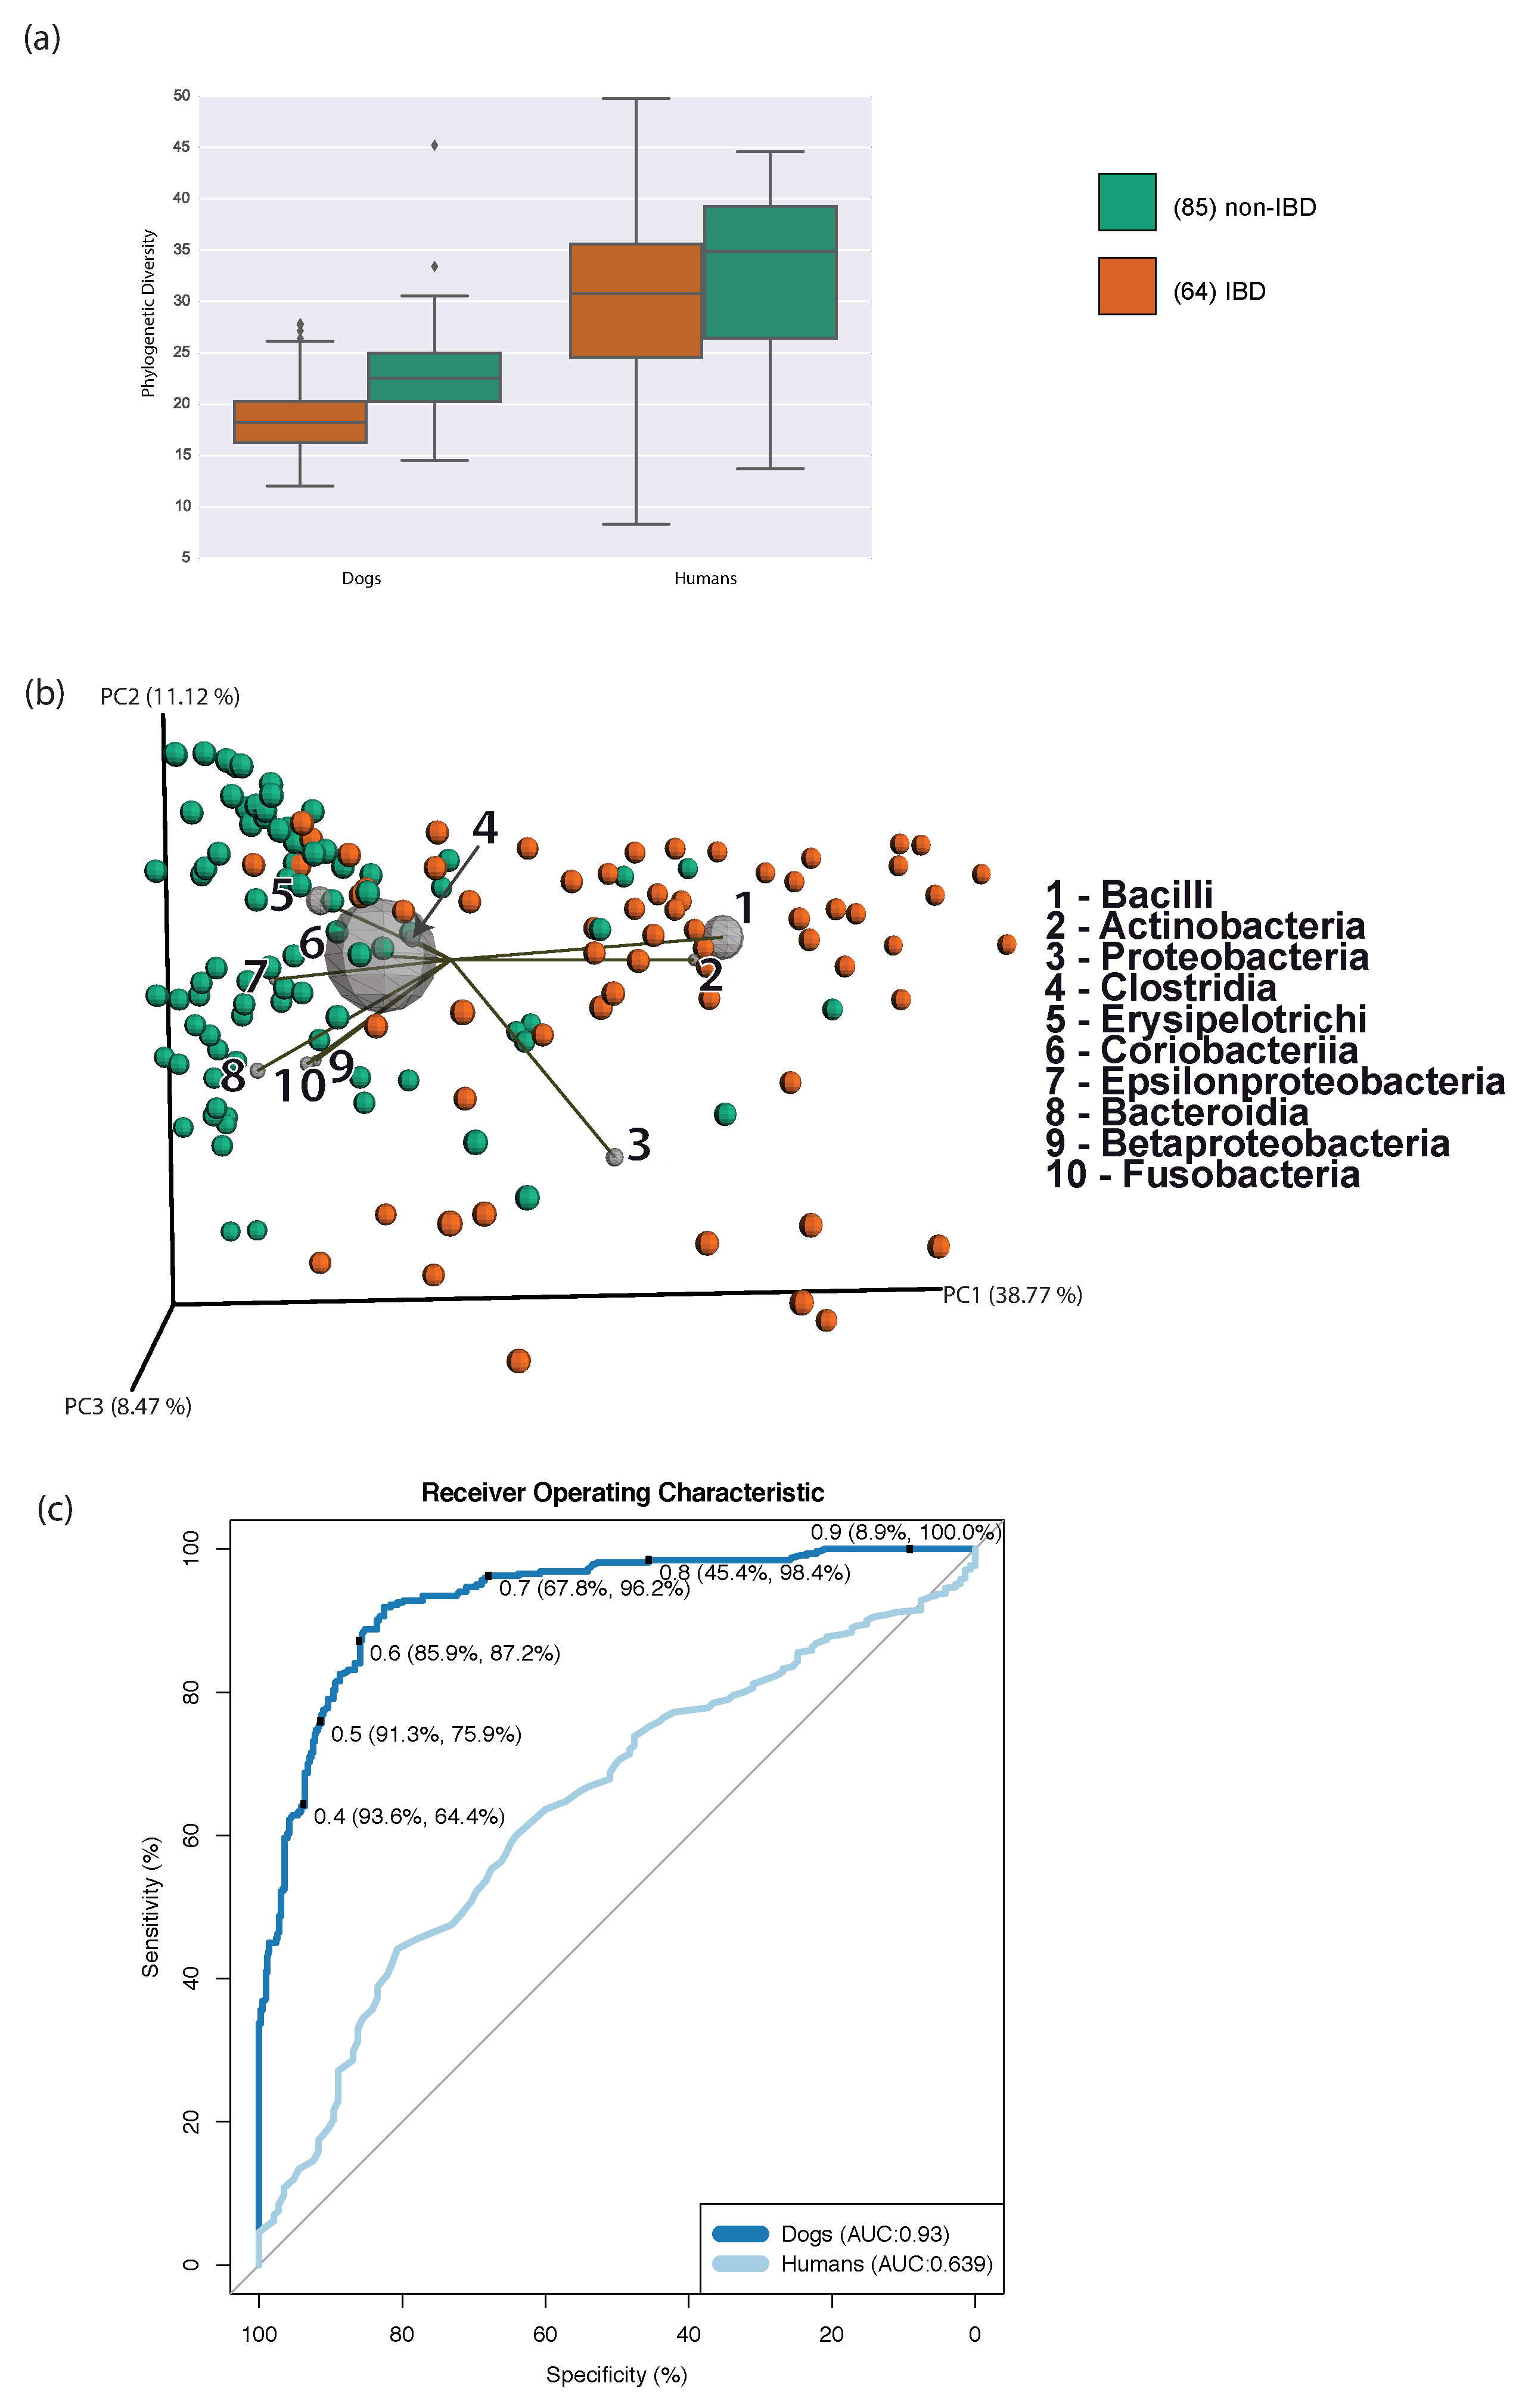
\includegraphics[height=0.85\textheight]{dogs-figures/figure-1}
\label{dogs_fig1}
\caption[Diversity overview and a comparison against humans.]{\textbf{Diversity overview and a comparison against humans.} (a) Comparison between disease states and species of Faith's phylogenetic diversity (whiskers extend for 1.5 times the \gls{iqr} past the low and high quartiles). (b) Weighted UniFrac beta diversity biplot, for the dog samples colored by disease status. (c) Performance comparison of a random forest classifier trained to separate the healthy from the diseased samples in both humans and dogs.}
\end{figure}

A random forests classifier \cite{RN4205} trained on the dog data achieved an \gls{auc} of 0.93 (Figure~\ref{dogs_fig1}C, see discriminant \glspl{otu} in Supplementary Table~1\footnote{\url{https://images.nature.com/original/nature-assets/nmicrobiol/2016/nmicrobiol2016177/extref/nmicrobiol2016177-s1.pdf}}), demonstrating excellent classification accuracy compared to human stool samples where the \gls{auc} was only 0.63 using a much larger training set \cite{RN154}, and achieved only \gls{auc} = 0.86 even using mucosal biopsies. Consequently, in dogs, but not in humans, high classifier accuracy is achievable for \gls{ibd} using only stool samples.

Encouraged by these results, we tested whether a dysbiosis (see supplemental methods) network trained on stool samples alone could be used to interpret the pattern of \gls{ibd} in dogs, and whether this pattern overlapped the human network. We previously found that in humans, substantially better correlation networks could be achieved from the mucosal biopsies, because many taxa contributing to these networks were not seen in stool. Accordingly, we used the techniques described \cite{RN154} to generate correlation networks and a dysbiosis index for dog samples (see supplemental methods for more information). Using the network together with the biplots (Figure~\ref{dogs_fig1}B) we see that Gammaproteobacteria (specifically \textit{Enterobacteriaceae}) were significantly associated with \gls{ibd}, whereas various Firmicutes such as Clostridium and \textit{Ruminococcus} were associated with non-\gls{ibd} samples. When these features are compared with the discriminant \glspl{otu}, obtained from the random forests classifier, we observe a general overlap of the lineages (see Supplementary Table 1 and Supplementary Table 2\footnote{\label{sup}\url{https://images.nature.com/original/nature-assets/nmicrobiol/2016/nmicrobiol2016177/extref/nmicrobiol2016177-s1.pdf}}). However we also see \glspl{otu} that are not highlighted by the correlation network. Specifically Erysipelotrichaceae \textit{Allobaculum} and Lachnospiraceae \textit{Blautia producta}, this is likely because these do not consistently co-occur with or co-exclude other taxa.

The human dysbiosis index failed to negatively correlate with alpha diversity in dog samples (Figure~\ref{dogs_fig2}A.1 and A.2 correlation, A.3 \gls{pcoa} plot), while a dog-specific dysbiosis index showed a statistically significant negative correlation in the same samples (Figure~\ref{dogs_fig2}B.1 and 2 B.2 correlation, C.3 \gls{pcoa} plot, see for a reference the two groups in Figure~\ref{dogs_fig2}D). Additionally we tested the index with previous data \cite{RN153}, and although the sample size is limited, we observed similar patterns (see Supplementary Figure 2\textsuperscript{\ref{sup}}). Similarly to humans, the dysbiosis index in dogs is negatively correlated with phylogenetic diversity (r = -0.45, p $<$ 0.001). However, the list of `non-\gls{ibd}' (co-occurring in non-\gls{ibd} samples) and `\gls{ibd}' (co-occurring in \gls{ibd} samples) bacteria only partially overlaps between host species (see Supplementary Table~2\textsuperscript{\ref{sup}}). Comparing the correlation networks of the taxa for humans (as described in \cite{RN154}) and the network generated for the dog data (Figure~\ref{dogs_fig2}C) revealed overlapping, and discordant taxa. In particular, \textit{Fusobacterium} appears to be associated with \gls{ibd} \cite{RN154} and colorectal cancer \cite{RN3983} in humans but with non-\gls{ibd} dog samples. Of note, we previously observed high levels of \textit{Fusobacterium} sp. in dogs \cite{RN150} but also carnivores of multiple species \cite{RN8250, RN114}, and noted higher levels of \textit{Fusobacterium} in dogs with more access to the outdoors \cite{RN4082}, which may correlate with a wide intake of other immunomodulatory environmental bacteria. Given the limited adaptation (approximately 8.9 Mya when humans split from Gorillas \cite{RN3988}) of the human lineage (historically omnivorous \cite{RN3987}) to a carnivorous diet, as compared to the base of the Carnivora 40-45 Mya \cite{RN3989}, it is possible that this taxon has yet to be incorporated into the non-\gls{ibd} portion of the network in humans. Nonetheless, it is important to remember this is only a statistical association, and further research would need to be developed to properly validate this. Consistent between human and canine networks and former studies were findings in regards to decreased \textit{Faecalibacterium} and increased \textit{Escherichia coli} in \gls{ibd} \cite{RN17138}, and these taxa seem to be important in this disease across animal hosts. Other taxa (\textit{Enterococcus} and \textit{Allobaculum}) from the canine network that were associated with \gls{ibd} or non-\gls{ibd} are generally consistent with previous results based on either small scale studies or targeted \gls{pcr} \cite{RN153}, but additional taxa were discovered here, such as \textit{Butyricoccus} which was associated with non-\gls{ibd} dogs.

\begin{figure}[htbp]
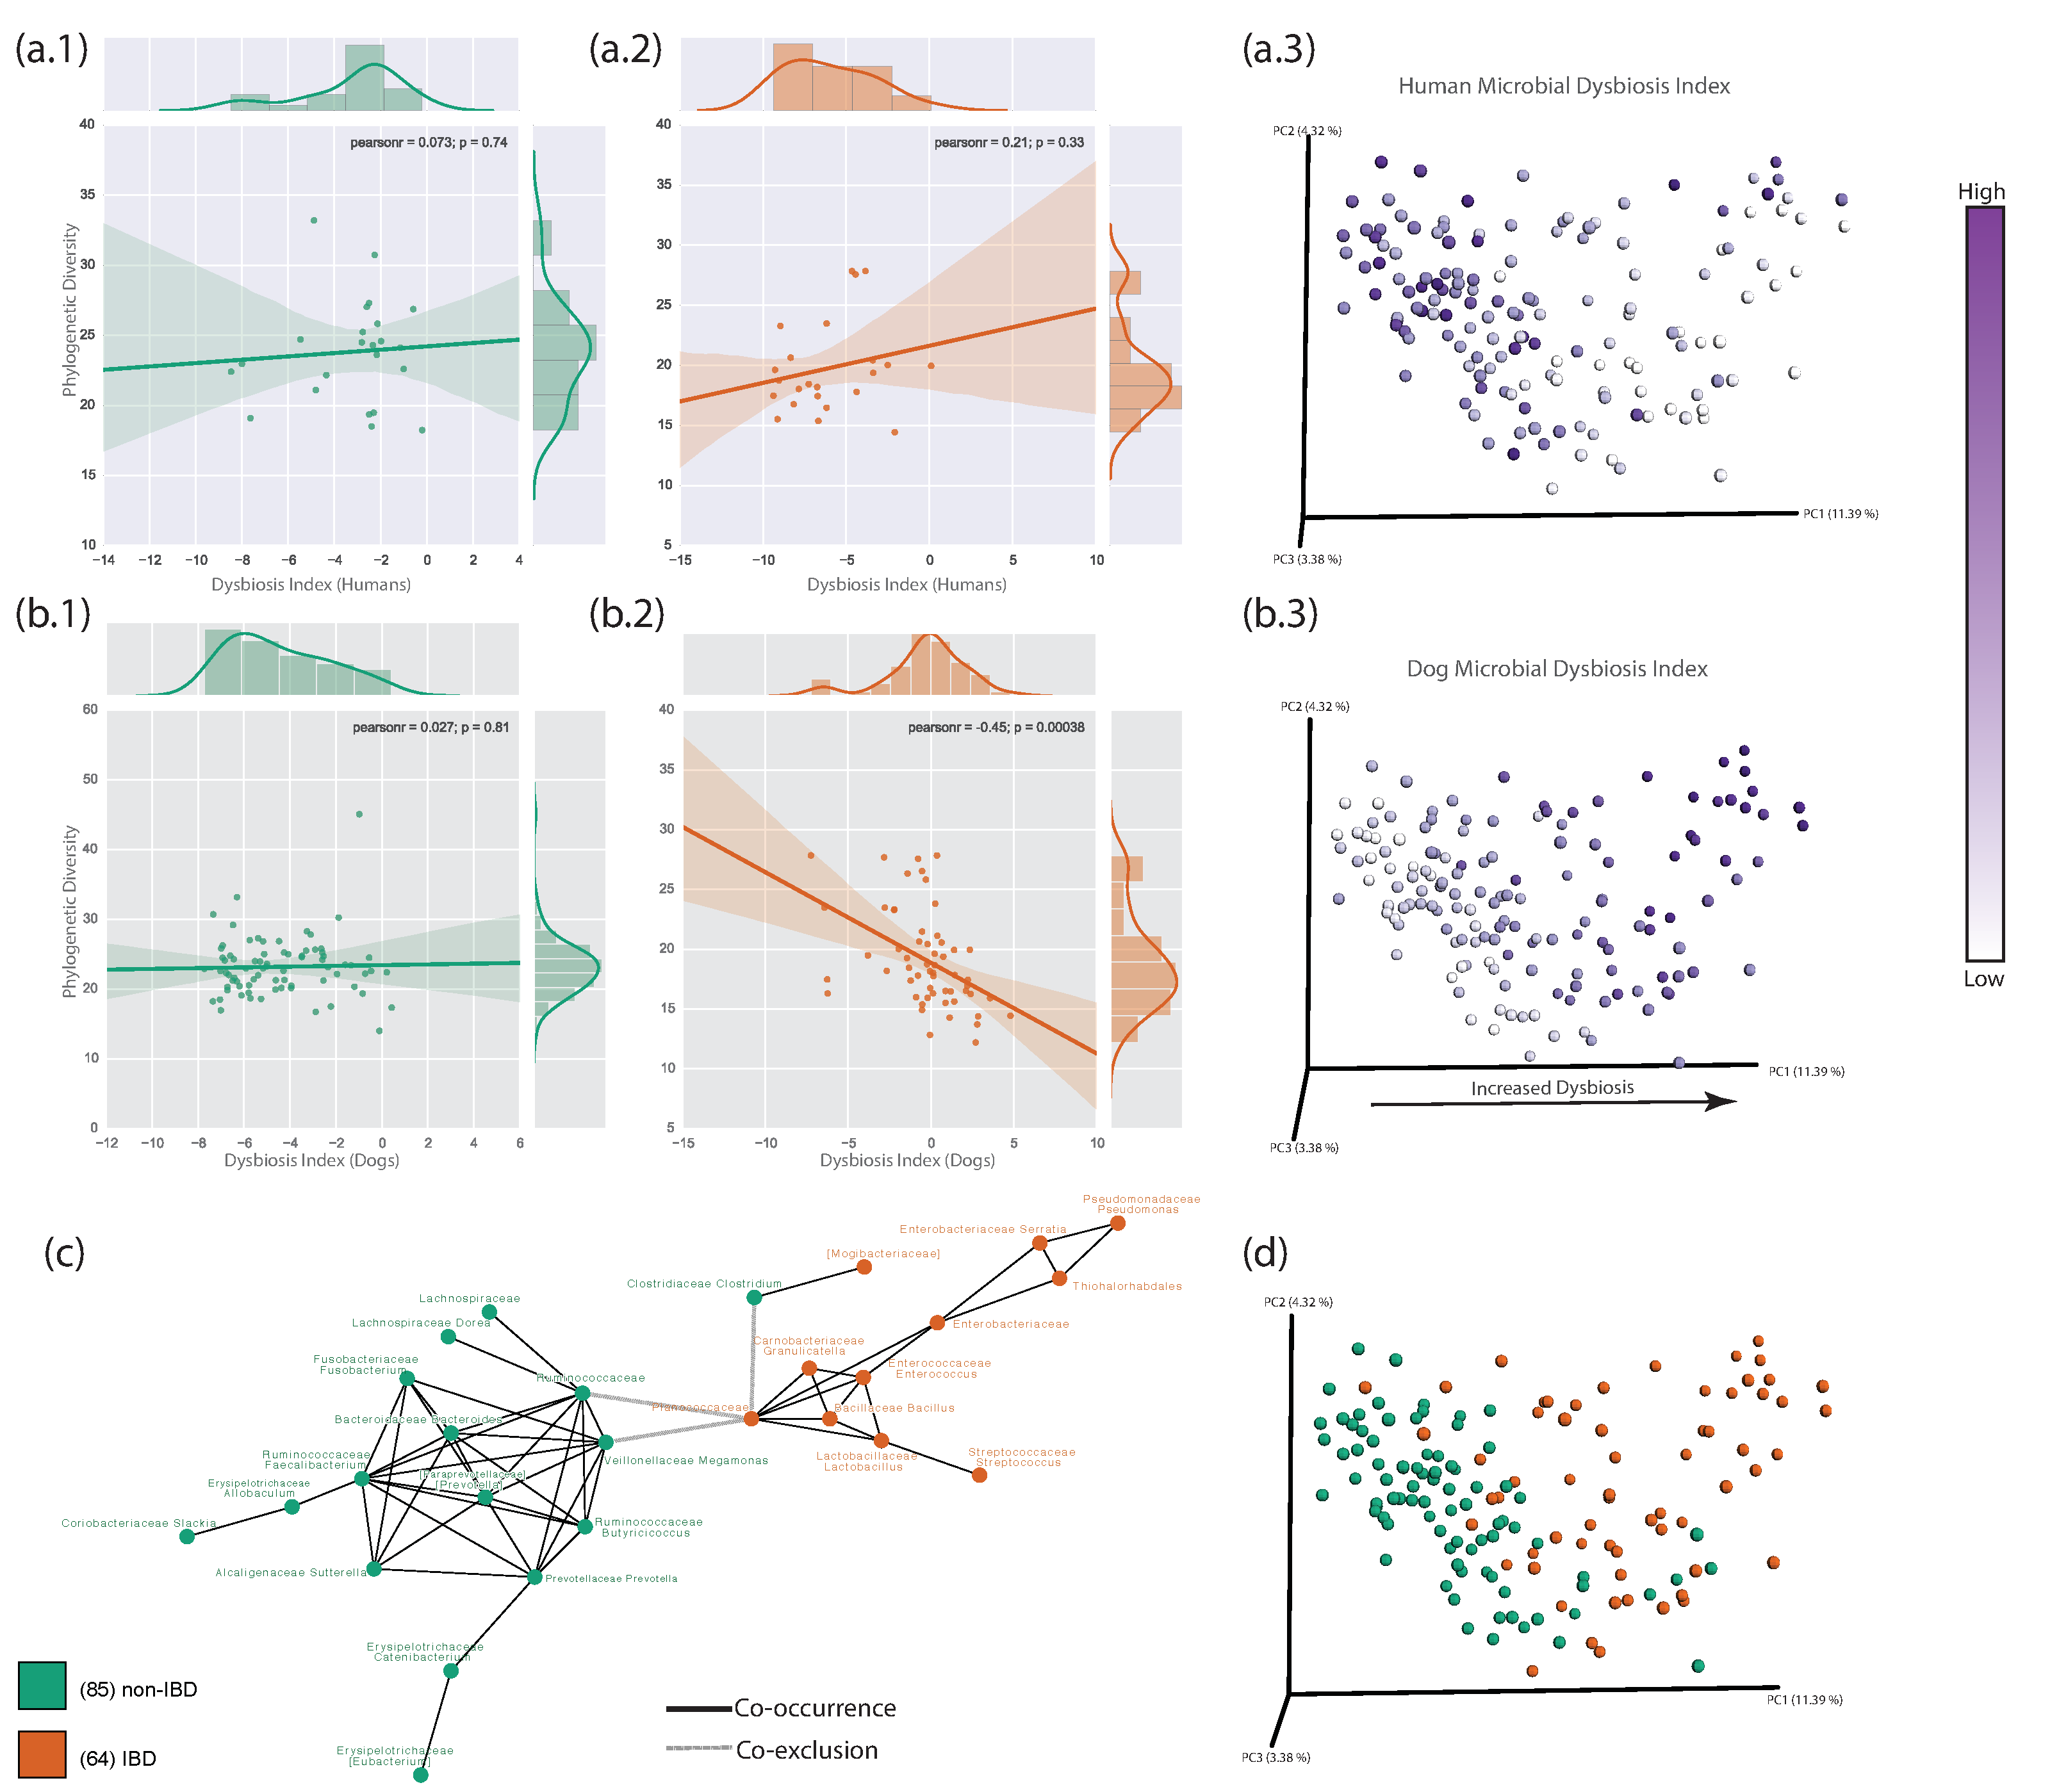
\includegraphics[width=1\columnwidth]{dogs-figures/figure-2}
\label{dogs_fig2}
\caption[Human and dog dysbiosis index.]{\textbf{Human and dog dysbiosis index.} (a.1), (a.2) Human dysbiosis index describing the dog samples grouped by disease status, (a.3) weighted UniFrac PCoA plot colored by dysbiosis index. (b.1) and (b.2) Dog dysbiosis index describing the dog samples grouped by disease state, (b.3) weighted UniFrac PCoA plot colored by dysbiosis index. (c) Correlation network used to determine the dysbiosis index in dogs, colored by the bacteria associated with IBD and non-IBD samples, co-exclusion edges are showed in dotted lines and co-occurrence edges are showed in solid lines. (d) Unweighted UniFrac PCoA plot of the dog data. Figures a.1, a.2, b.1 and b.2 all display 95\% confidence intervals.}
\end{figure}

To measure the relative effect size of host-species and \gls{ibd}, we combined humans and dogs into a single \gls{pcoa} plot, marked by clinical status (Supplementary Figure~4\footnote{\label{sup2}\url{https://images.nature.com/original/nature-assets/nmicrobiol/2016/nmicrobiol2016177/extref/nmicrobiol2016177-s1.pdf}}). We demonstrate that at a microbial level the disease effect is smaller than the host effect (human vs. dog, Supplementary Figure 4 A\textsuperscript{\ref{sup2}}). Similarly the disease effect was weaker than the species effect when analyzing PICRUSt \cite{RN17472} metagenome prediction data (\gls{permanova} test grouping samples by disease status and by host-species using a binary Jaccard matrix, p=0.001, pseudo-F by disease 14.61, pseudo-F by species 52.59, Supplementary Figure 4 B\footnote{\label{sup3}\url{https://images.nature.com/original/nature-assets/nmicrobiol/2016/nmicrobiol2016177/extref/nmicrobiol2016177-s1.pdf}}), indicating that at both the compositional and predicted functional level, species is a more significant influence on the microbial community than disease (see supplemental methods and Supplementary Figure~3\textsuperscript{\ref{sup3}}). In both dogs and humans, predicted pathways were relatively similar across \gls{ibd} and non-\gls{ibd} samples, with the most abundant pathways across both groups in both species including `housekeeping' pathways such as transporters, ABC transporters, DNA repair and recombination proteins, ribosome, purine metabolism, transcription factors, peptidases, pyrimidine metabolism, and chromosome (Supplementary Figure~5\textsuperscript{\ref{sup3}}). Although these most abundant pathways were not significantly associated with health or disease, the abundance of several lower abundance pathways was significantly different across \gls{ibd} and non-\gls{ibd} samples in dogs, see Supplementary Table~3\textsuperscript{\ref{sup3}}. No pathways were significantly higher in between disease statuses in humans.

Taken together, these results have important implications for translational medicine and for understanding \gls{ibd} in dogs. Also, the major functional gene content was conserved across non-\gls{ibd} and \gls{ibd} humans and dogs. While some significant predicted functions were identified between non-\gls{ibd} and \gls{ibd} dogs, the human sample population did not have enough non-\gls{ibd} individuals analyzed for proper statistical power. This together with previous work suggests similar functional changes within the microbiota of dogs and humans with \gls{ibd}. Previous studies have already shown that some treatment approaches to \gls{ibd} that target the microbiome are conserved across dogs and humans, such as antibiotics, dietary modulation, and probiotics. For example, specific probiotic therapy has been shown to have similar effects on fecal and mucosa-adherent microbiota and host immune response (i.e., increase of tight junction proteins, increase in beneficial mucosa-adherent bacteria) in humans, dogs, and rat models of colitis \cite{RN17583, RN17357, RN158}. 
Our study also revealed that the dysbiosis networks clearly differ in some key bacterial groups. Better understanding of the similarities in these microbial networks and functional changes may extend the abilities to test therapeutic approaches across multiple host species.

\subsection{Methods}

Naturally passed fecal samples were analyzed from 85 healthy dogs and 65 dogs with chronic signs of gastrointestinal disease and confirmed inflammatory changes on histopathology. All dogs participated in different clinical studies and leftover fecal samples were utilized for this study. The protocol for sample collection was approved by the Clinical Research Review Committee of the College of Veterinary Medicine, Texas A\&M University (CRRC\#09-06). 

Dogs with clinical signs of chronic \gls{gi} disease (i.e., vomiting, diarrhea, anorexia, weight loss, etc.) were diagnosed with idiopathic \gls{ibd} based on the\gls{wsava} criteria: (i) chronic (i.e., $>$ 3 weeks) GI signs; (ii) histopathologic evidence of mucosal inflammation; (iii) inability to document other causes of GI inflammation; (iv) inadequate response to dietary, antibiotic, and anthelmintic therapies, and (v) clinical response to anti-inflammatory or immunosuppressive agents.  Histological samples were obtained endoscopically. The clinical status of each dog was evaluated using a published clinical \gls{cibdai}. Within the \gls{ibd} dogs, 41 dogs had histological confirmed inflammation in the small intestine, 18 dogs had histological changes in both small intestine and colon, and 5 dogs had only histological changes reported in the colon. Histological changes were predominantly of lymphoplasmacytic infiltrates, with a subset of dogs also showing eosinophilic and/or neutrophilic components. The mean (SD) \gls{cibdai} for \gls{ibd} dogs was 6.4 (3.1).

Dogs were excluded if they received antibiotics within the past 2 weeks of sample collection. Data on antibiotic history was nevertheless collected: 34/65 dogs with \gls{ibd} had no history of prior antibiotics administration, while 13 dogs received antibiotics several weeks ($>$2) or months before sample collection. The remaining 18 dogs in the \gls{ibd} group had no information about prior antibiotic use. In the healthy group (n=85), 76 dogs had not received any antibiotics, and 9 dogs had a history of antibiotic use, but not within the last 2 weeks of sample collection. No technical replicates were generated in this study.

Sample and animal information (i.e., age, weight, gender, breed, duration of clinical signs, histopathology, antibiotic usage) was obtained from clinical records. Also, if the owner provided the information, the exact diet (trade name and manufacturer) fed at time of sample collection was recorded in the clinical records, and the dietary macronutrients (protein, fat, and carbohydrate content) were recorded from manufacturer's provided data on the labels.

Body weights ranged from 2.9 to 55 kg (mean 22 kg, SD: 14.9 kg), which was not significantly different from (Mann Whitney test; p=0.087) the healthy dogs (range 0.9 to 50 kg; mean 20.3 kg, SD: 10.7g). Mean age (SD) was 5.4 (3.07) in the \gls{ibd} group, which was not significantly (Mann Whitney test; p=0.311) different from healthy dogs (4.7, 3.2). There was a wide breed distribution with 37 different breeds in the \gls{ibd} group and 42 different breeds in the control group. In the \gls{ibd} group, Yorkshire terrier, German Shepherd dogs and Labrador Retrievers (n=5 each) were most commonly represented.

\Gls{bcs} were assessed according to the \gls{wsava} criteria. \Gls{bcs} is rated in a 9-point scale that visually evaluates a dog's body composition. This score has been validated against the standard \gls{dexa} \cite{RN4000}. For this dataset, the \Gls{bcs} was restricted to a subset of the healthy samples, therefore \gls{ibd} vs. Healthy comparisons could not be made in this case.

\subsubsection{DNA Extraction and Sequencing}

DNA isolation was performed as described by the Earth Microbiome Project Protocol (version 4\textunderscore 13) for 16S rRNA\cite{RN164}. The full cohort included 192 samples, of which 15 were removed because those subjects had acute hemorrhagic diarrhea, and had little clinical information available. The remaining 28 samples did not recover enough sequences after quality control including screening for low counts of reads per sample. All samples were sequenced using the Illumina HiSeq platform (2 x 100 nucleotide sequences and an index read).

\subsubsection{Data Processing}

Demultiplexed and quality controlled sequences were then clustered against the Greengenes \cite{RN165} database (release 13\textunderscore 8) using the closed reference \gls{otu} picking protocol \cite{RN81} as implemented in \gls{qiime} \cite{RN110} 1.9.0; these processing steps were performed using the default parameters. The \gls{otu} table used for primary analysis was filtered to include only samples from subjects that presented inflammatory bowel disease or that were healthy controls. Blank samples, and subjects with diarrhea were removed. Finally the table was rarefied to normalize for sampling effort \cite{RN167} at 15,000 sequences per sample, this cutoff was selected as having the best trade-off between sequences and samples per disease status category.

Samples from \cite{RN153} were processed with the same pipeline as described above, except these were rarefied at 4,500 sequences per sample.

To address the differences in sequencing length, the combination of samples with the human dataset \cite{RN154} was preceded by trimming the sequences to an even 100 nucleotides per sequence, the rest of the pipeline was performed as described above. The same \gls{otu} picking protocol and reference database were used, therefore allowing the combination of the studies using the \gls{otu} tables. We only used the fecal samples from the human dataset.

\subsubsection{Statistical analysis}

Jupyter Notebooks \cite{RN162} with the analysis of this dataset are available on online\footnote{\url{https://www.github.com/ElDeveloper/dogs}}. Briefly, alpha and beta diversity calculations of weighted and unweighted UniFrac \cite{RN83} were performed using \gls{qiime} version 1.9.1. To assess statistical significance in these comparisons we used \gls{permanova}, grouping the samples by disease status (healthy vs \gls{ibd}), p=0.001 in both cases; pseudo-F statistics were 9.46 for unweighted UniFrac and 39.65 for weighted UniFrac. \gls{roc} curves and feature importance were calculated using Caret \cite{RN3986} and hack\textunderscore ml \footnote{\url{https://github.com/RNAer/hack_ml}}.

Statistical significance between diversity distributions were calculated using Mann-Whitney's test, linear regressions and correlation coefficients were calculated using NumPy 1.10.4 \cite{RN3823} and SciPy version 0.17, and visualized using Seaborn 0.7.0 \cite{RN170}. Principal coordinates analysis plots were created using Emperor 0.9.51-dev~\cite{RN79}.

Metagenome predictions were performed using the Galaxy implementation of PiCRUST version 1.9.0. Significant differences in predicted KEGG Pathways between healthy and \gls{ibd} groups were calculated using a Kruskal-Wallis test with multiple corrections (FDR and Bonferroni corrected p-values). The 16S data is comprised of 85 healthy dogs, 64 \gls{ibd}-affected dogs, 29 healthy humans and 450 humans with \gls{ibd}. On the other hand the PICRUSt predicted data is comprised of 85 healthy dogs, 42 \gls{ibd}-affected dogs, 23 healthy humans and 344 humans with \gls{ibd}.

The Jaccard distance was used to compare the PICRUSt predicted data. This metric compares the samples on a presence/absence basis, and is not concerned with the similarity in the abundances of the \glspl{otu} but rather with the overlap in their presence. Each value is computed as one minus the ratio of shared \glspl{otu} to total \glspl{otu} present in the two samples.

To assess the quality of the predictions in the dog samples, we computed the `nearest sequenced taxon index' (see Supplementary Figure S3\footnote{\url{https://images.nature.com/original/nature-assets/nmicrobiol/2016/nmicrobiol2016177/extref/nmicrobiol2016177-s1.pdf}}), and verified that the samples had acceptable values (below 0.15).

\subsubsection{Dysbiosis Network}

The dysbiosis network was calculated as described in \cite{RN154}, using CCREPE \cite{RN168} and visualized using Cytoscape \cite{RN169}. The index is calculated by taking the log transform of the abundance of the ratio of \gls{ibd}-associated microbes to non-\gls{ibd} associated microbes as determined by the correlation network.

This network is created by first scoring the co-occurrence and co-exclusion patterns in the samples. CCREPE uses a compositionally adjusted version of the checkerboard score \cite{RN3985}; the results are filtered to remove non-statistically significant relationships, and to preserve the largest connected component only. We represent the results as a graph where vertices are microbes and edges are interaction types. Vertices are of one of two classes (\gls{ibd}-associated and Healthy-associated) as determined by the class where they were dominantly abundant, and edges between vertices have a weight given by their adjusted checkerboard score (negative values represent co-exclusions, and positive values represent co-occurrences). The specifics of this processing are described in the supplemental Jupyter notebooks.

\subsubsection{Accession Numbers}

Raw sequences for the dog samples have been deposited to the \gls{ena} at the following accession number ERP014919, equivalent processed \gls{otu} tables and metadata can be accessed through Qiita\footnote{\label{qiitaurl}\url{https://qiita.microbio.me}} under study 833 - `Dog models of inflammatory bowel disease'.

The data for the human dataset\cite{RN154} can be found in the \gls{ena} at the following accession numbers ERP015241 and ERP015242, equivalent processed \gls{otu} tables and metadata can be accessed through Qiita\textsuperscript{\ref{qiitaurl}} under study identifiers 1939 and 1998 -`The Treatment-Naive Microbiome in New-Onset Crohn's Disease'.

Data for the additional dog study \cite{RN153} can be found at the \gls{sra} of the under accession number SRP040310.

\subsubsection{Conflict of Interest}
We declare none.

\subsubsection{Author Contributions}
Y. V. B. wrote the manuscript, managed, interpreted and analyzed the data. E. H. contributed to the manuscript and analyzed the data. J. S. contributed to the manuscript, analyzed and interpreted the data. R. K. wrote the manuscript and interpreted the data. All authors worked together to finalize and approve this manuscript.

Please direct all material and requests to Rob Knight robknight@ucsd.edu.

\subsubsection{Acknowledgments}

We wish to acknowledge the support provided by the Crohn's and Colitis Foundation of American; the Templeton Foundation and the Keck Foundation (via the Earth Microbiome Project), the National institutes of Health. We wish to thank Zhenjiang Xu, Jon Sanders, Amnon Amir, Gail Ackermann, Jamie Morton, Luke Ursell, Jessica Metcalf, Antonio Gonzalez and Emma Schwager for their useful comments and feedback in the writing of this manuscript. 

\else
    \section{IBD dogs paper}\label{dogs}
\fi

\chapter{Dynamic features of inflammatory bowel disease}\label{chapter_ibds}

In recent years, clinical research in \gls{ibd} has benefited from multi-'omic 
(genomic \cite{RN4217}, metabolomic \cite{RN4264}, and metagenomic 
\cite{RN4263}) characterizations of the condition. Each of these approaches 
describes a new component of relationships that, one by one, seem to uncover 
the processes regulating the inflammation and well-being of the affected hosts.  
Nonetheless, longitudinal descriptions (and as a consequence representations) 
of \gls{ibd} were largely unexplored.

This chapter introduces two pioneering longitudinal studies of \gls{ibd}. One 
where the sampling is sparse (every three months) and another where the 
sampling is dense (as much as every day). Both cohorts present increased rates 
of microbial variation. Specifically, we see that this appears to be different 
for the different subtypes of \gls{ibd}. In order to visualize the increased 
variation, we rely on the techniques introduced in 
Chapter~\ref{exploratory_chapter}, and on the definition of a reference plane 
that acts as a proxy for healthy variation.

Motivated by these findings, we use an unsupervised classification model to 
determine the benefits of increased longitudinal sampling. For both 
(independently collected and sequenced) datasets, we observe that including 
more than one sample per subject increases the performance of a classifier.  
This property is only possible when we transform the original representation of 
the data and create per-subject consensus features based on multiple 
timepoints. Briefly, these features aggregate multiple samples together and 
exploit the increased instability as an informative classification feature.

Although we exercise and test this method with human-gut data, the approach is 
not restricted in any way to this environment. This approach could potentially 
benefit other applications, specially where longitudinal descriptors might be 
predictive of a state of interest.

% TODO: add publication
Section~\ref{section_plane} appeared in \textsl{Nature Microbiology, 2017}. My 
role in this project was to act as the lead analyst of the project, I developed 
a collection of new algorithms to represent the data, produced a series of 
visualizations used in the paper, co-wrote the text, and interpreted the 
results. Section~\ref{section_ibd} appeared in the journal \textsl{Gut, 2017}.  
As the lead contributor of this project, I co-wrote the text, generated the 
main figures, wrote the software used for analysis, interpreted the results, 
and deposited the data into a public repository.

\ifdefined\RELEASE
    \glsresetall

\section{Dynamics of the human gut microbiome in Inflammatory Bowel Disease}

\subsection{Abstract}

Inflammatory bowel disease (IBD) is characterized by flares of inflammation with periodic need for increased medication and sometimes even surgery. \gls{ibd} etiology is partly attributed to a deregulated immune response to gut microbiome dysbiosis. Cross-sectional studies have revealed microbial signatures for different \gls{ibd} diseases, including \gls{uc}, \gls{ccd}, and \gls{icd}. Although \gls{ibd} is dynamic, microbiome studies have primarily focused on single timepoints or few individuals. Here we dissect the long-term dynamic behavior of the gut microbiome in \gls{ibd} and differentiate this from normal variation. Microbiomes of v subjects fluctuate more than healthy individuals, based on deviation from a newly-defined \gls{hp}. \Gls{icd} subjects deviated most from the \gls{hp}, especially subjects with surgical resection. Intriguingly, the microbiomes of some \gls{ibd} subjects periodically visited the \gls{hp} then deviated away from it. Inflammation was not directly correlated with distance to the healthy plane, but there was some correlation between observed dramatic fluctuations in the gut microbiome and intensified medication due to a flare of the disease. These results help guide therapies that will re-direct the gut microbiome towards a healthy state and maintain remission in \gls{ibd}.

\subsection{Results and Discussion}

Both the state and the dynamics of the human gut microbiome in healthy individuals are highly personalized \cite{Costello2009,Eckburg2005,Flores2014,Human2012,Martinez2013,Qin2010,RN4120,Zaura2015}. Although cross sectional studies have revealed dysbiosis of the gut microbiome in \gls{ibd} \cite{Gevers2014,Rajca2014,Sokol2008,Willing2009,Willing2010}, little is known about the individual nature of microbiome dynamics in \gls{ibd}, beyond a study of 3 \gls{uc} patients before and after ileostomy, and two small studies of \gls{ibd} patients in remission or during changes in disease activity \cite{Martinez2008,Wills2014,Young2013}.  Here we studied the long-term dynamics of the gut microbiome from an \gls{ibd} cohort of 128 individuals (49 \gls{cd}, 60 \gls{uc}, 4 \gls{lc}, 15 \gls{cc}) and 9 \gls{hc}. We sampled at three-month intervals, collecting 1–10 samples per individual for a total of 683 samples (Supplementary Table~1\footnote{\label{suppdf}\url{https://images.nature.com/original/nature-assets/nmicrobiol/2017/nmicrobiol20174/extref/nmicrobiol20174-s1.pdf}}). The microbiome composition in each sample was determined by sequencing the V4 region of the 16S rRNA gene for a total of 248 million 16S rRNA gene amplicons. To determine links between the gut microbiome and clinical factors, we collected clinical data, including fecal calprotectin (f-calprotectin) concentration and surgical resection status. To control sampling bias, we restricted our statistical analyses of volatility to a subset of the cohort that had sequence data from the first four time points and that had matching f-calprotectin concentrations; yielding 276 samples from 69 patients (Supplementary Table 1\textsuperscript{\ref{suppdf}}, Supplementary Dataset~1\footnote{\url{https://images.nature.com/original/nature-assets/nmicrobiol/2017/nmicrobiol20174/extref/nmicrobiol20174-s2.txt}}); results were similar when all subjects were considered). We also included patient \gls{gls} based on 163 known \gls{ibd} risk loci for 29 patients to assess potential links between the host genetics, \gls{ibd} and the microbiome \cite{Jostins2012}. 

As expected from previous work \cite{Gevers2014,Willing2010}, we found that \gls{hc} and \gls{ibd} subtypes formed distinct clusters by \gls{pcoa} of unweighted UniFrac distances, with \gls{icd} patients least similar to healthy controls (Supplementary Figure~1\textsuperscript{\ref{suppdf}}), ADONIS stratified by time point, p $<$ 0.001). As in previous studies \cite{ Rajca2014,Willing2010,Wills2014}, we found differences in alpha and beta diversity of the microbiome according to \gls{ibd} subtype and between subtypes and healthy controls and identified several families that correlated with health or disease state, e.g. \textit{Enterobacteriaceae} with \gls{icd} and \textit{Ruminococcaceae} with \gls{hc} (Supplementary Figure 1-2\footnote{\label{supPdf2}\url{https://images.nature.com/original/nature-assets/nmicrobiol/2017/nmicrobiol20174/extref/nmicrobiol20174-s1.pdf}}).  Individual taxa that are differentially abundant between \gls{ibd} subtypes compared to \gls{hc} are listed in Table~\ref{plane-tab1} (DESeq2, log2 fold change). The \gls{ibd} microbiomes contained significantly lower abundances of putative beneficial \glspl{otu} present in \gls{hc}, as previously reported \cite{Gevers2014,Rajca2014,Sokol2008,Willing2009,Willing2010,Wills2014}, including \textit{Prevotella copri} and the butyrate-producing bacterium \textit{Faecalibacterium prauznitzii} (Table~\ref{plane-tab1}; Supplementary Figure~3\textsuperscript{\ref{supPdf2}}).

\begin{table}[htbp]
\renewcommand{\arraystretch}{0.6}% Tighter
\centering
\caption{Differential abundance in specific taxa according to disease phenotype comparisons (DESeq2)}
\label{plane-tab1}
\scalebox{0.8}{\begin{tabular}{ccccc}
\toprule
Groups compared &	BaseMean &	log2FoldChange &	padj &	Taxonomic annotation\\
\midrule
ICD-r over ICD-nr &	13,32&	-7,05&	0,0000000&	\textit{Faecalibacterium prausnitzii}\\
&	4,08&	-5,57&	0,0000011&	Lachnospiraceae\\
&	3,32&	-5,08&	0,0000001&	Ruminococcaceae\\
&	6,49&	-5,40&	0,0000009&	Ruminococcaceae\\
&	19,85&	-6,11&	0,0000005&	Ruminococcaceae\\
&	94,87&	-5,87&	0,0000001&	Ruminococcaceae\\
&	53,59&	-8,10&	0,0000012&	\textit{Ruminococcaceae Ruminococcus}\\
&	72,13&	-5,14&	0,0000241&	Clostridiales\\
\midrule
ICD-r over HC&	14,91&	7,20&	0,0000000&	Alteromonadales [Chromatiaceae]\\
&	13,32&	-7,22&	0,0000000&	\textit{Faecalibacterium prausnitzii}    \\
&	2,94&	-5,34&	0,0000007&	Ruminococcaceae\\
&	2,33&	-5,62&	0,0000000&	Clostridiales\\
&	10,41&	-7,47&	0,0000000&	Lachnospiraceae\\
&	15,12&	-7,62&	0,0000001&	Lachnospiraceae \textit{Coprococcus}  \\
&	4,13&	-8,43&	0,0000000&	Lachnospiraceae\\
&	19,85&	-7,15&	0,0000000&	Ruminococcaceae\\
&	5,43&	-8,72&	0,0000000&	Ruminococcaceae\\
&	7,16&	-6,98&	0,0000151&	Clostridiales\\
&	3,78&	-6,69&	0,0000249&	Clostridiales\\
&	2,10&	-6,53&	0,0000000&	Ruminococcaceae\\
&	5,76&	-7,85&	0,0000000&	Ruminococcaceae\\
&	53,59&	-8,64&	0,0000000&	Ruminococcaceae \textit{Ruminococcus}\\
&	72,13&	-5,71&	0,0000000&	Clostridiales\\
&	121,13&	-9,95&	0,0000000&	\textit{Prevotella copri}\\
&	5,87&	-7,58&	0,0000000&	\textit{Methanobrevibacter}\\
\midrule
ICD-nr over HC&	14,91&	6,47&	0,0000185&	Alteromonadales [Chromatiaceae]\\
&	2,94&	-7,00&	0,0000756&	Ruminococcaceae\\
&	5,43&	-8,17&	0,0000682&	Ruminococcaceae\\
&	121,13&	-7,82&	0,0000185&	\textit{Prevotella copri}\\
\midrule
CCD over HC&	5,43&	-8,65&	0,0000000&	Ruminococcaceae\\
&	121,13&	-7,94&	0,0000000&	\textit{Prevotella copri}\\
\midrule
UC over HC&	6,53&	6,32&	0,0000978&	\textit{Alistipes massiliensis}\\
\bottomrule
\multicolumn{5}{p{18cm}}{Criteria for inclusion: BaseMean $>$ 1 and padj $<$ 0.0001. Brackets indicate putative taxonomy based upon phylogenetic placement as given in the Greengenes taxonomy. BaseMean is the mean of normalized counts for all samples. padj is the Benjamini–Hochberg adjusted p-value.}
\end{tabular}}
\end{table}

From the animated ordination of the samples (Supplementary Video 1\footnote{\label{supVideo}\url{https://images.nature.com/original/nature-assets/nmicrobiol/2017/nmicrobiol20174/extref/nmicrobiol20174-s3.mov}}), we observed that although microbiome samples from the healthy individuals varied over time, they were restricted to a small volume of the ordination space. In contrast, \gls{ibd} subtypes traversed far more of the total volume, sporadically visiting the area where healthy samples resided. To summarize these dynamics, we identified a `healthy plane' (hereafter referred to as \gls{hp}). Briefly, this plane is calculated in a space derived from \gls{pcoa} of unweighted UniFrac distances of healthy subjects (Supplementary Video 1\textsuperscript{\ref{supVideo}}). We constructed a model using the samples from the \gls{hc} patients, and fit them to a two-dimensional plane embedded in a three-dimensional space using the least squares method (Figure~\ref{plane-fig1}). The plane is then restricted to only span the three-dimensional ranges of the \gls{hc} samples. This plane was used as a proxy to represent the normal microbial variation within healthy subjects and to summarize the abnormal, intermittent dysbiosis associated with \gls{ibd}.

\begin{figure}[htbp]
\includegraphics[height=0.6\textheight]{plane-figures/Fig1}
\caption[Defining a healthy plane.]{\textbf{Defining a healthy plane.} Diagram summarizing the procedure for creating a representative plane for a group of samples S: \textbf{a}, sample selection, \textbf{b}, model fitting and \textbf{c}, distance calculations for all samples. The healthy plane is then located in UniFrac space by \textbf{d}, fitting a line to the major axis of the points, and \textbf{e}, defining a least-squares fit to identify a plane that minimizes the sum of squares of distances to the nearest point on the plane. \textbf{f}, Verification that the position of the healthy plane is not driven by proteobacteria-dominated outliers: Procrustes Analysis comparing original samples and those with Proteobacteria removed. A vector connects each original sample (red) with the same samples after Proteobacteria have been omitted (black). p $<$ 0.001, M\textsuperscript{2} = 0.018, 999 permutations. \textbf{g}, The short length of most vectors indicates that the relative composition of most samples does not change when proteobacteria are filtered out.}
\label{plane-fig1}
\end{figure} 

The procedure was as follows: let S be a set of n samples $s_1,s_2,… s_n$ corresponding to a group of trajectories, each trajectory pertaining to a subject with at least four samples collected at distinct points in time. Each sample is represented as a three-dimensional vector corresponding to sample coordinates in ordinated space i.e. $s_1=(x_1,y_1,z_1); s_2=(x_2,y_2,z_2); … s_n=(x_n,y_n,z_n)$. We fit a linear model to $S$ by the least squares method to obtain coefficients for the equation of a three dimensional surface $T$, next we restricted a segment of this surface to the ranges given by $[min_x (S),max_x (S)]$ and $[min_y (S),max_y (S)]$, we defined this to be a plane representative of $S$ or $P_s$. When $S$ is the set of samples from healthy subjects in an ordination space we, refer to $P_s$ as the \gls{hp}. Finally, we defined $d_k$ to be the Euclidean distance from a sample $k$ to the nearest point lying on $P_s$. After measuring $d_k$ for all samples in our study, we grouped samples according to their diagnosis, and compared the distributions of distances. Figure~\ref{plane-fig1} a-c demonstrates this procedure, and Figure~\ref{plane-fig1} d-e demonstrates the placement of the \gls{hp} in the context of our full \gls{ibd} dataset. Samples from the \gls{hp} are co-located with one another, while many samples from \gls{ibd} patients are further away. To investigate whether this effect is due to `outlier' groups of samples that are dominated by taxa that are typically rare in healthy individuals, we excluded all Proteobacteria from the dataset, and compared the location of samples in unweighted UniFrac space with and without Proteobacteria using Procrustes analysis. As shown in Figure 1f-g, the omission of Proteobacteria is significant (p $<$ 0.01), but this effect is largest in the already dysbiotic \gls{icd}-r patients and aligns with PC3. The effect on healthy controls is minimal, and healthy samples are still located only near the \gls{hp} (Figure~\ref{plane-fig1} f-g).

Calculation of the mean Euclidean distance from each sample to the \gls{hp} revealed that all subtypes of \gls{ibd} significantly deviated from the \gls{hp} (\gls{glm}, all p $<$ 0.00268, Figure~\ref{plane-fig2}a). Samples from patients with \gls{ccd} and \gls{uc} were closer to the \gls{hp}, and some samples did not differ significantly from healthy controls, whereas \gls{icd} samples were the most distant from the \gls{hp} (Supplementary Video 1\footnote{\label{supVideo2}\url{https://images.nature.com/original/nature-assets/nmicrobiol/2017/nmicrobiol20174/extref/nmicrobiol20174-s3.mov}}; Figure~\ref{plane-fig2}). The highest volatility was observed for \gls{icd} patients that had previously undergone ileocecal resection (\gls{icd}-r), followed by \gls{icd} patients without surgery (\gls{icd}-nr) based on UniFrac distances between successive samples (Figure 2b). \gls{icd}-r patients also had low gut microbial richness (Supplementary Figure~2\footnote{\label{suppdfFig}\url{https://images.nature.com/original/nature-assets/nmicrobiol/2017/nmicrobiol20174/extref/nmicrobiol20174-s1.pdf}}). Ileocecal resection is a major modifier of intestinal physiology, and the observed pronounced volatility in \gls{icd}-r patients might be partly explained by removal of the ileocecal valve per se. Ileal inflammation may also influence bile salt uptake and, consequently, colonic transit time and microbiome volatility. Interestingly, several \gls{ibd} patients had complex trajectories that sporadically moved to and from the \gls{hp} (Figure~\ref{plane-fig2}c, Supplementary Video~1\textsuperscript{\ref{supVideo2}}).

\begin{figure}[htbp]
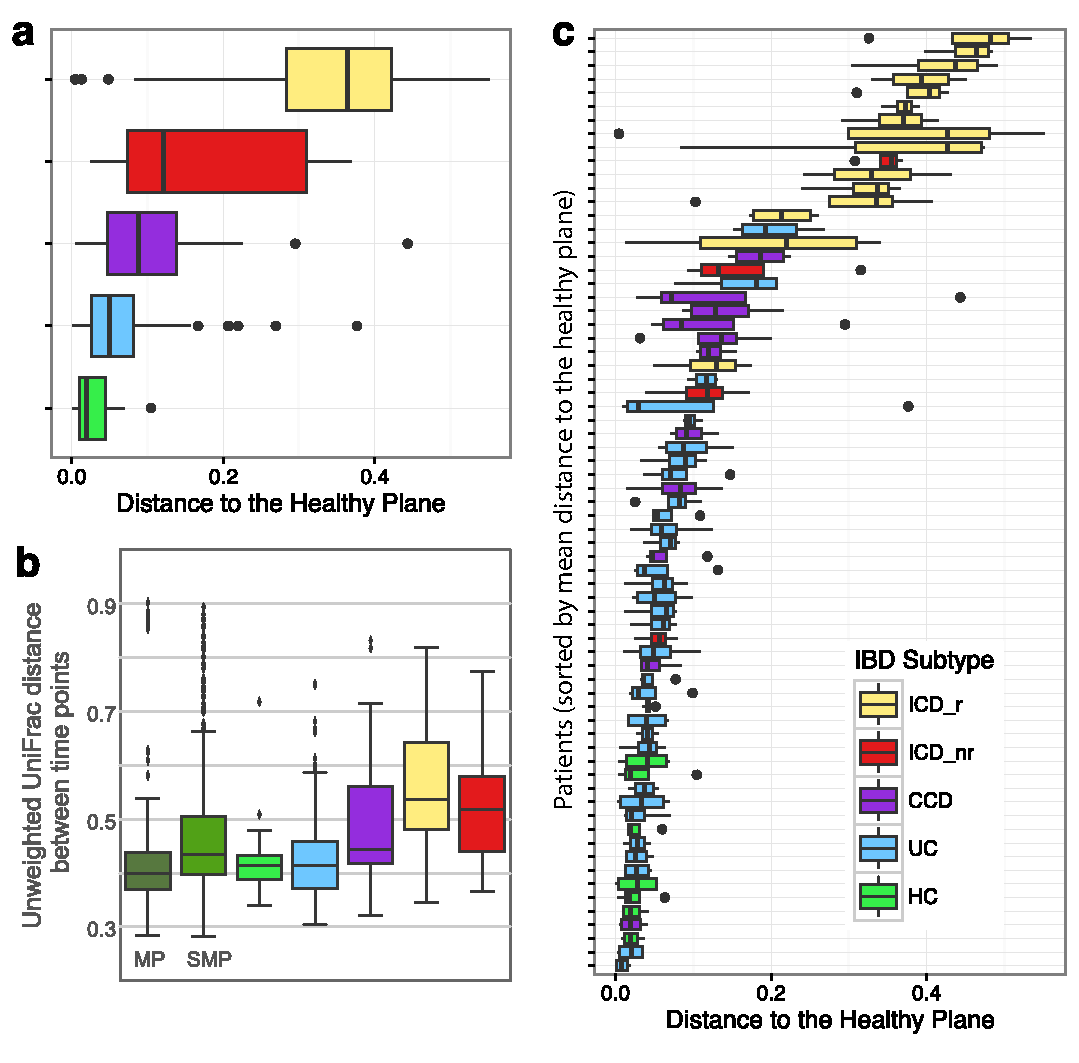
\includegraphics[width=\columnwidth]{plane-figures/Fig2}
\caption[The gut microbiomes of different IBD subtypes display different distributions relative to a healthy plane (HP)]{\textbf{The gut microbiomes of different IBD subtypes display different distributions relative to a healthy plane (HP). a}, Median distances from HP for each IBD subtype. All IBD subtypes were significantly different from healthy controls (GLM, all p $<$ 0.00261). b, UniFrac distances between subsequent samples. c, Distance to HP for each individual patient. HP was defined using data shown in Supplemental~Video 1\textsuperscript{\ref{supVideo2}}. See Supplementary Table~1\textsuperscript{\ref{suppdfFig}} for composition of downstream analysis cohort. Boxes show interquartile range (IQR). Whiskers denote the lowest and highest values within 2.5 × IQR of the median. Circles represent outliers.}
\label{plane-fig2}
\end{figure} 

Although our study represents the largest longitudinal analysis of the \gls{ibd} microbiome to date, the small number of patients in specific subgroups limited some statistical comparisons. Furthermore, the number of healthy controls was lower than the number of \gls{ibd} patients. To address this limitation of unequal sampling of healthy individuals and \gls{ibd} patients, we compared the volatility of our healthy controls to healthy participants in two published studies, the \gls{smp} and the \gls{mp} datasets \cite{Caporaso2011genbiol,Flores2014}. There was less variability over time in healthy individuals across all three cohorts compared to those with \gls{ibd} (Figure 2b). This result emphasizes that \gls{ibd} is characterized by volatile dysbiosis not found in healthy people, and confirms earlier preliminary results and meta-analysis of much smaller studies \cite{Manichanh2012,Martinez2008,Wills2014,Young2013}.

To extend our understanding of the mechanisms underlying the microbiome dynamics, we explored the correlation between the dynamics and inflammatory activity in each sample using f-calprotectin $>$ 150 $\mu$g/g as a surrogate for inflammatory activity. The concentration of f-calprotectin in stool samples has previously been correlated with endoscopic and histopathologic activity, and is used in daily clinical practice because it is non-invasive \cite{Lewis2011}. We observed that concentrations of f-calprotectin were higher in all \gls{ibd} subtypes than in healthy controls (Figure~\ref{plane-fig3}). However, we did not observe a significant correlation between f-calprotectin and distance from the \gls{hp}  (Figure~\ref{plane-fig3}, \gls{glm} p = 0.275). Although recent microarray analyses of the gut microbiome in a cohort of anti-TNF treated pediatric \gls{ibd} patients\cite{Kolho2015} and experiments with gnotobiotic fecal transplants suggest that microbial composition and function are causally associated with inflammatory activity \cite{Rooks2014}, our differential abundance testing revealed only weak trends and no specific \glspl{otu} that varied significantly with active inflammation, using f-calprotectin $>$ 150 $\mu$g/g as cut-off. However, the use of f-calprotectin as a proxy for inflammatory activity might have introduced bias, because f-calprotectin is a less accurate marker of ileal than colonic inflammation \cite{Sipponen2008} and \gls{icd} patients displayed the greatest distance from the \gls{hp}.

Examples of the microbiome dynamics for one representative \gls{hc} and one from each \gls{ibd} subgroup are shown in addition to changes in f-calprotectin concentrations, distance to \gls{hp}, and Shannon diversity in Figure~\ref{plane-fig4} (all individual profiles are shown in Supplementary Figure~3\footnote{\label{suppdf3}\url{https://images.nature.com/original/nature-assets/nmicrobiol/2017/nmicrobiol20174/extref/nmicrobiol20174-s1.pdf}}), illustrating the more stable dynamics over time for \gls{hc} and \gls{uc} compared to the other clinical phenotypes of \gls{ibd}, with the most fluctuations occurring for patient 69 that had undergone surgical resection. The f-calprotectin levels were low and relatively stable for the \gls{hc} compared to the \gls{ibd} patient (Figure~\ref{plane-fig4}). In these examples, there were also substantial fluctuations in diversity for the \gls{hc}, \gls{icd}-r, and \gls{ccd} by contrast to \gls{uc} and \gls{icd}-nr patients.

\begin{figure}[htbp]
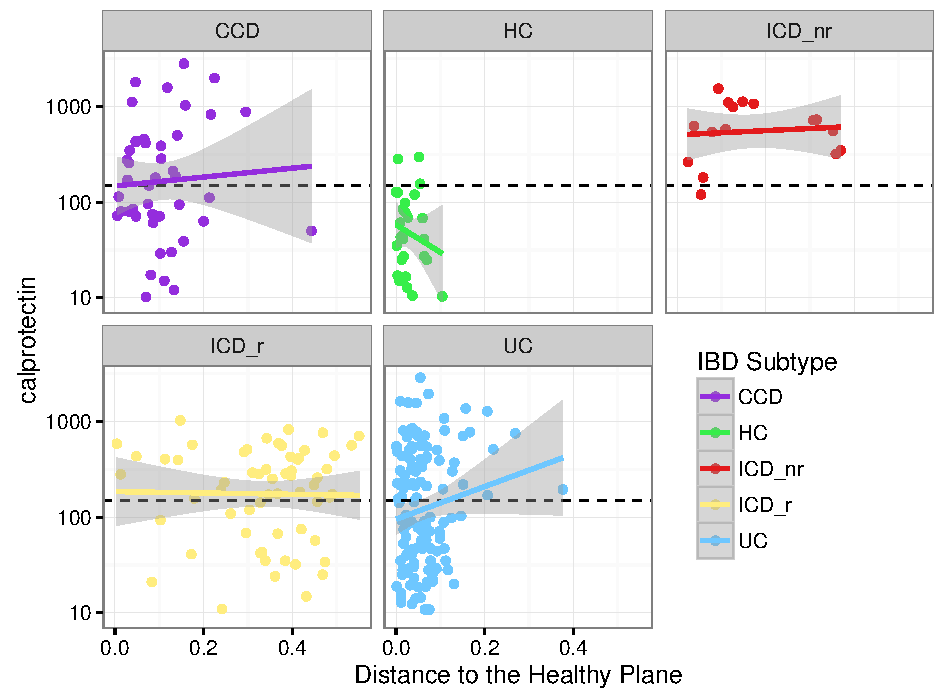
\includegraphics[width=\columnwidth]{plane-figures/Fig3}
\caption[Correlation between fecal calprotectin concentrations and distance to a defined healthy plane (HP) in 3D ordination space.]{\textbf{Correlation between fecal calprotectin concentrations and distance to a defined healthy plane (HP) in 3D ordination space.} Data represent a correlation of f-calprotectin levels and distance to the here defined healthy plane in 3D ordination space (see Supplementary Video~1\textsuperscript{\ref{supVideo2}}) for each individual and time point for different inflammatory bowel disease (IBD) subtypes. To compare the relationship between f-calprotectin and the healthy plane, a generalized linear mixed effects model was fit, with a conditional Gamma distribution, using f-calprotectin and disease type as fixed effects and including a random subject effect; f-calprotectin was not significant (p = 0.27501).}
\label{plane-fig3}
\end{figure} 

\begin{figure}[htbp]
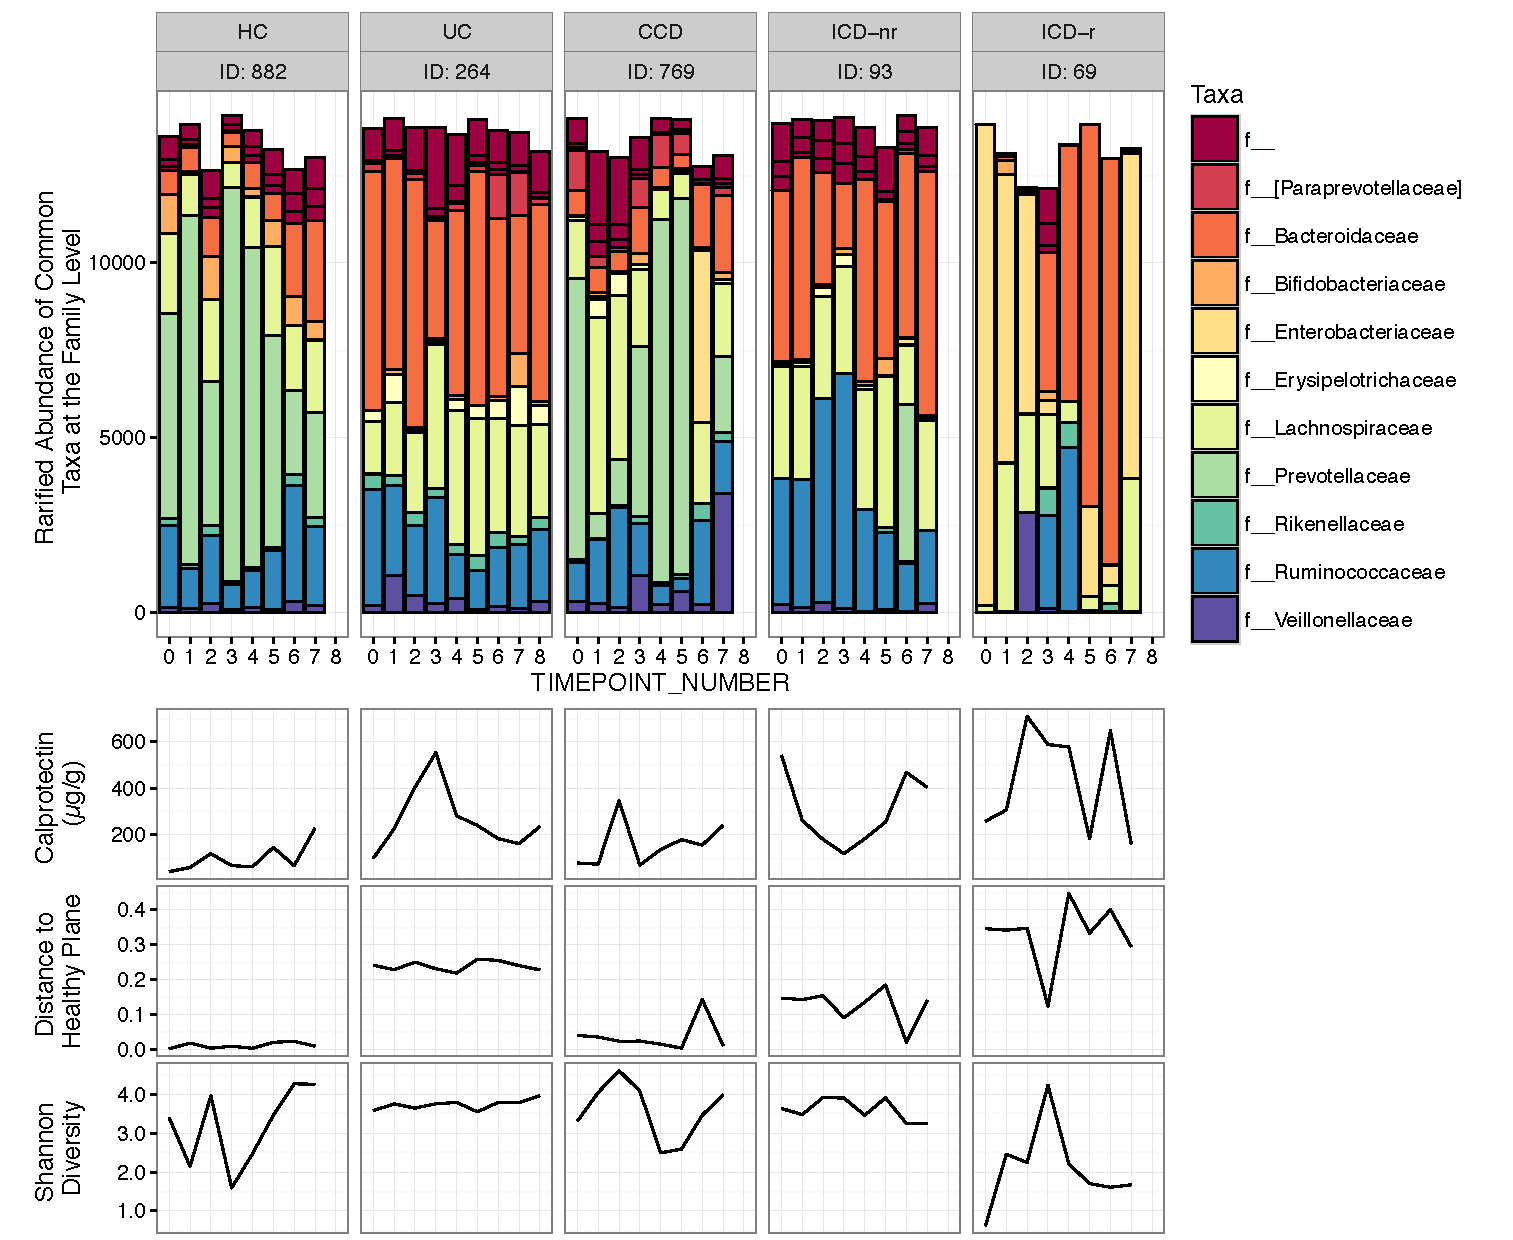
\includegraphics[width=\columnwidth]{plane-figures/Fig4}
\caption[Microbiome dynamics of selected individuals from each IBD subtype and a healthy control.]{\textbf{Microbiome dynamics of selected individuals from each IBD subtype and a healthy control.} From each IBD subtype and healthy control group, representative individuals sampled over the most time points and having complete clinical and sequence data were selected. Data represent f-calprotectin values, distance to the healthy plane, and Shannon diversity and rarified abundances of most common taxa at the family level. Note that taxa unclassified at the family level are represented in the ‘f\textunderscore' category.}
\label{plane-fig4}
\end{figure} 

We further explored the individual dynamics of the gut microbiome in \gls{ibd} patients who experienced increased clinical disease activity, according to the physician's global assessment (Supplementary Figure~4\textsuperscript{\ref{suppdf3}}). Recently, the short-term (6 weeks) dynamics of the microbiome in pediatric patients with active \gls{ibd} treated with anti-TNF indicated that initiation of medical treatment changes the microbial composition at the genus level \cite{Kolho2015}. Because we had few anti-TNF exposed patients, and our patients received a course of corticosteroids at flare as first line therapy, we explored how corticosteroid administration influenced microbiome dynamics. Our data demonstrate that change in medication influenced the volatility of the microbiome (Supplementary Figure~4\footnote{\url{https://images.nature.com/original/nature-assets/nmicrobiol/2017/nmicrobiol20174/extref/nmicrobiol20174-s1.pdf}}). Patients receiving a course of oral corticosteroids (n=7) had more microbiome fluctuations than patients on stable medication (n=49), based on calculations of unweighted UniFrac distance between time points (Wilcoxon Signed-rank test; p=0.04). Our dynamic model suggests that beyond the association with \gls{ibd} subtype and the weak correlation with inflammation, the dynamics of the microbiome composition are influenced by changes in medication. The extent to which other factors, such as dietary changes and smoking, may have influenced the observed volatility remains speculative, because the collected information was insufficiently detailed to include these factors as covariates.

To evaluate the microbiome as a predictive tool, we combined the microbial and clinical data and used a supervised learning Random Forests model to predict \gls{ibd} subtypes \cite{Breiman,Love2014}. To avoid overfitting, our models were built using \gls{otu} abundances from the first time points only, along with clinical metadata (\gls{bmi}, f-calprotectin concentrations, sex, and Distance to the \gls{hp}). Accuracy was evaluated using the remaining three time points, which were not used to train the model. Using this model, the \gls{ibd} subtypes were discriminated from healthy controls and correctly predicted for 66.6\% of samples (Supplementary Table~2\footnote{\label{suppdf4}\url{https://images.nature.com/original/nature-assets/nmicrobiol/2017/nmicrobiol20174/extref/nmicrobiol20174-s1.pdf}}), consistent with the findings reported in Gevers et al. (2014). Feature importance scores from this model revealed several potential microbial indicators of \gls{ibd} subtypes, including \glspl{otu} matching to \textit{Lachnospira}, \textit{Clostridium}, \textit{Oscillospira}, and many unidentified \textit{Ruminococcaceae} (Supplementary Table~3\textsuperscript{\ref{suppdf4}}). Intriguingly, the accuracy of the model increased slightly if f-calprotectin concentrations were omitted, but decreased by at least 10\% if the distance to the \gls{hp} was removed (Supplementary Tables 2 and 3\textsuperscript{\ref{suppdf4}}), suggesting that the \gls{hp} is a more important factor in the model. Comparable levels of accuracy were previously achieved using rectal samples \cite{Gevers2014}, but here we show that the same can be achieved with fecal samples, which are easier to collect. When immunochip data were included for a subset of 29 \gls{ibd} individuals and the Random Forests model was repeated, the samples were still classified into the four \gls{ibd} subtypes (\gls{uc}, \gls{ccd}, \gls{icd}-r, \gls{icd}-nr) (Supplementary Tables 2 and 3\textsuperscript{\ref{suppdf4}}). While distance to the \gls{hp} remained as the single most important feature for classification,\gls{gls} were more predictive than sex, f-calprotectin, or \gls{bmi} when included in the model (Supplementary Table~2\textsuperscript{\ref{suppdf4}}). However, including \gls{gls} only increased the overall accuracy of the model by about 2\%, demonstrating the predictive potential of the microbiome. Interestingly, in a recent study of obesity covering 339,224 individuals, the 97 risk loci for obesity accounted for only 2.7\% of \gls{bmi} variation \cite{Locke2015}, whereas the microbiome classified lean from obese individuals with 90\% accuracy \cite{Knights2011}, providing precedent for the predictive value of the gut microbiome over human genetics in chronic disease.

In summary, by analyzing fecal samples collected every 3 months from a large \gls{ibd} cohort, we determined the long-term volatility of the gut microbiome in \gls{ibd}. Our data revealed that although the microbiome of healthy individuals varied it was only within a newly defined \gls{hp}, whereas there was considerable volatility away from the \gls{hp} for several of the \gls{ibd} cohorts. Devising improved methods to detect the healthy state with non-invasive sampling, to predict when the healthy state will be departed, and to sustain the microbiome in this healthy state by erecting barriers that prevent the slip back into dysbiosis, will be an important focus of future work.


\subsection{Methods}

\subsubsection{Cohort Demographics}

Patients with \gls{cd} or \gls{uc}, the two major forms of \gls{ibd}, attending the outpatient clinic were consecutively invited to take part. After obtaining written consent, \gls{bmi} was recorded and patients were asked to provide a fecal sample and to fill in a questionnaire with clinical disease activity, present medication, dietary habits, use of antibiotics and use of \glspl{nsaid}. Disease phenotype was classified according to the Montreal classification \cite{Silverberg2005}. Individuals were then followed prospectively, asked to provide fecal samples and to fill in the questionnaire every third month for a two-year period. If a patient did not provide a fecal sample at any of the three months periods, a reminder letter was sent. In total 109 patients with \gls{ibd} (\gls{cd}; n=49 and \gls{uc}; n=60) took part. Nine additional individuals with no \gls{ibd} or any other gastrointestinal conditions were recruited as \gls{hc} as well as 19 patients with other chronic inflammatory gastrointestinal diseases (4 \gls{lc} and 15 \gls{cc}).  All 137 individuals were Caucasians and together they provided 683 fecal samples during the two-year period (Supplementary Table~4\footnote{\url{https://images.nature.com/original/nature-assets/nmicrobiol/2017/nmicrobiol20174/extref/nmicrobiol20174-s1.pdf}}). The study was approved by the Ethical Committee of the Medical Faculty, Uppsala University (2007/291).

\subsubsection{Sample Collection}

Fecal samples were self-collected in sterile plastic containers and stored at -80 °C until shipping on dry ice and processing.

\subsubsection{Fecal calprotectin} 

To assess the degree of inflammatory activity at the collection of each fecal sample, the concentration of f-calprotectin was assessed by commercially available ELISA, Calprotectin Elisa Buhlmann Laboratories AG, Basel, Switzerland, according to the manufacturer's protocol. 

\subsubsection{DNA Extraction and Amplification}

Genomic DNA was extracted from 0.25 g of fecal material from each sample using the Earth Microbiome DNA extraction protocol \cite{EMP2011}. Briefly, DNA was extracted using the 96-well format MoBio Powersoil DNA kit on an EpMotion 5075 robot with vacuum (Eppendorf, Hamburg, Germany). DNA was quantified with the Qubit 2.0 fluorometer (Invitrogen, Carlsbad, CA) according to the manufacturer's instructions.

PCR amplification and library preparation were performed similarly to the protocol described by Caporaso et al. \cite{Caporaso2011proceedings}. 515F/806R Illumina primers with unique reverse primer barcodes were used to target the V4 region of the 16S rRNA gene. Samples were amplified in triplicate and cleaned using the MO BIO 69 htp PCR cleanup kit. Each PCR reaction included 1X PCR buffer, 10 $\mu$M each forward and reverse primer, 200 μM dNTPs, 1 U/ml Taq polymerase, 15 ng template DNA, and PCR grade water, with a total reaction volume of 25 $\mu$L. Reactions were kept at 94\textdegree C for 3 minutes for denaturation to occur. Amplification was performed by 25 cycles of 94\textdegree C for 45s, 58\textdegree C for 60s, and 72\textdegree C for 90s. The V4 amplicons were sequenced on the Illumina HiSeq 2000 platform, yielding single end, 100 base pair reads. Sequencing and quality assessment were performed at the Yale Center for Genome Analysis.

\subsubsection{Phylogenetic Analysis}

Sequence data were processed using QIIME 1.9.0-dev through the online platform QIITA\footnote{\url{https://qiita.ucsd.edu}}\cite{ Caporaso2010}. Four HiSeq lanes of data were demultiplexed with default quality filtering settings and subsequently combined, resulting in 248,547,926 total sequences. These sequences were clustered using SortMeRNA at 97\% identity against the Greengenes rRNA reference database May 2013 release \cite{Kopylova2012,McDonald2012}. Sequences that failed to match the database were discarded. 237,653,256, or approximately 95.6\% of the sequences, clustered against the Greengenes reference dataset. Even sampling was performed at 14,553 sequences per sample for beta diversity and supervised learning analyses. The beta diversity principal coordinates plot of unweighted UniFrac distances was constructed using the same rarefied \gls{otu} table, and visualized in Emperor \cite{Lozupone2005,Vazquez2013}. Clinical matched metadata, including f-calprotectin concentrations, were included when available. From each patient, the first four microbiome samples with matched f-calprotectin concentrations were sub-selected for use in downstream analysis. 

\subsubsection{Statistical Analysis.}

The R package phyloseq was used to import and graph data, while the packages DESeq2, randomForest, and vegan were used to perform differential abundance testing and supervised learning \cite{Ihaka1996,Liaw2002,Love2014,McMurdie2013,Oksanen2016}. Statistical significance of unweighted UniFrac distance matrices comparing healthy controls and \gls{ibd} subtypes was assessed using the ADONIS test. The variation of the microbial community over time was calculated with vector lengths produced by summing the total distance between each subject's time points over the first three \gls{pcoa} axes of unweighted UniFrac space. The Random Forests model was constructed using the first time point from each patient in the downstream analysis cohort and prediction accuracy was measured using the subsequent three time points  (\gls{ccd} = 11 patients, \gls{icd} without resection (\gls{icd}-nr) = 4 patients, \gls{icd} with resection (\gls{icd}-r) = 15 patients, \gls{uc} = 30 patients, and \gls{hc} = 7 patients). The following metadata categories used as features for supervised learning: \gls{bmi}, f-calprotectin (continuous), sex, and Distance to the Healthy Plane. For classification on the subset of samples with immunochip data, the above process was used while adding \gls{gls}. We used a dataset of 29 \gls{ibd} samples (25 \gls{cd}, 4 \gls{uc}) with available immunochip data to estimate a \gls{gls} for each sample. In particular, \gls{gls} was calculated summing the number (counts) of risk alleles (0,1,2) at lead \gls{snp} from each \gls{ibd} risk locus (n = 163) according to Jostins et al. \cite{Jostins2012}.

After performing principal coordinates analysis of the unweighted UniFrac distance matrix, the samples of \gls{hc} were used to fit using the least squares method on the first three principal coordinates. The distance from each sample to this plane was measured and added to the sample metadata both for weighted and unweighted UniFrac. To compare distribution of samples relative to this healthy plane, a generalized linear mixed effects model was fit, with a conditional Gamma distribution, using disease type as a fixed effect and including a random subject effect.

To assess the variation between samples in an orderly manner (as described by the time point), we measured the UniFrac (weighted and unweighted) distance between samples that occur sequentially for any given subject; samples representing the final collection point do not have a value in these columns, as there is no subsequent sample to compare to.

We examined the power of differential abundance tests for the 16S data. DESeq2 \cite{Love2014} assumes that counts can be modeled as a negative binomial distribution with a mean parameter, allowing for size factors, and a dispersion parameter. The test for differential abundances fits a generalized linear model with a negative binomial family and a log link function. 

A power analysis was conducted by using samples from the downstream analysis cohort (Supplementary Table~4\footnote{\url{https://images.nature.com/original/nature-assets/nmicrobiol/2017/nmicrobiol20174/extref/nmicrobiol20174-s1.pdf}}). The power of the differential abundance test is dependent on the sample size of groups, difference in mean counts, type 1 error rate, and the dispersion value. Here we used a conventional type 1 error rate of 0.05 and assumed that we have two groups with sample sizes of n1 = 25 and n2 = 80. A total of 1000 \glspl{otu} were randomly selected from the data and dispersion parameters were estimated for each \gls{otu}. Data was then simulated from a negative binomial distribution, as specified by DESeq2, for each estimated dispersion value with means giving 2 fold, 1.5 fold, and 1.25 fold differences. For each mean fold difference value and dispersion value, a total of 5000 data simulations were done and a Wald test for difference in means using a generalized linear model was conducted. Based on these simulations, where data is generated with true differences, the fraction of times that the null hypothesis is correctly rejected (the power), was calculated and our comparisons were well powered given our subset sample sizes (Supplementary  Table~4\footnote{\url{https://images.nature.com/original/nature-assets/nmicrobiol/2017/nmicrobiol20174/extref/nmicrobiol20174-s1.pdf}}). 

\textbf{Data Availability:} Microbiome data from this study is available on Qiita under study ID 1629 (https://qiita.ucsd.edu/study/description/1629) and using the EBI accession number ERP020401. Patient clinical information is available on Qiita and in Supplemental Dataset~1\footnote{\url{https://images.nature.com/original/nature-assets/nmicrobiol/2017/nmicrobiol20174/extref/nmicrobiol20174-s2.txt}}. 

\textbf{Code Availability:} Our analysis methods make use of standard, open source software. R software packages are available on CRAN\footnote{\url{cran.r-project.org}}, bioconductor\footnote{\url{bioconductor.org}}, and GitHub\footnote{\url{github.com/joey711/phyloseq}}. Python software is available in the bioconda and biocore Conda channels, and is maintain on GitHub\footnote{\url{github.com/biocore, github.com/ElDeveloper/reference-plane}}.

    \glsresetall

\section{Guiding longitudinal sampling in inflammatory bowel diseases cohorts}

The volatile microbial signatures of\gls{cd} patients greatly hinder our ability to classify healthy from affected subjects using 16S rRNA profiles from stool. The recent work by Pascal et al. \cite{RN4208} overcomes this issue and other complications \cite{RN4219}, producing a decision tree that classifies subjects with \gls{cd}, \gls{uc}, irritable bowel syndrome and anorexia. Although the authors note that both subtypes of \gls{ibd}, particularly \gls{cd}, have increased microbial community instability, this information is not used as a feature to improve classifier accuracy. Could microbiome instability become actionable by creating a new classifier that benefits from repeated measurements? If so, how many samples per individual are needed to assess instability?

We collected daily stool samples for up to six weeks from 19 \gls{cd} subjects and 12 controls (see the analysis notebook for cohort description\footnote{\label{footlongibd}\url{https://github.com/knightlab-analyses/longitudinal-ibd}}) over 2 separate periods of 2 or 4 weeks spread over 2 and 5 months, for a total of 960 samples. We believe this is the most densely sampled longitudinal study of \gls{cd}; previous studies collected samples every 1-3 months \cite{RN4206, RN4208}. Our cohort shows decreased alpha diversity and increased stability, as previously reported in \gls{cd} and other subtypes of \gls{ibd} \cite{RN4217, RN140, RN4206, RN4208}.  We also noted that subjects who underwent resection have lower alpha diversity than other \gls{cd}-affected subjects (see analysis notebooks\textsuperscript{\ref{footlongibd}}).

A critical experimental design question for clinical studies is whether a finite budget should best be spent collecting samples from more patients, or collecting more serial samples from each patient? Therefore, we created a Random Forests \cite{RN4205} model based on per-subject aggregation of longitudinal data for alpha diversity \cite{RN4007}, beta diversity \cite{RN3770} and abundances of two phylogenetic factors found to be associated with \gls{cd} in ileal biopsies \cite{RN140, RN4204} (Figure~\ref{ibd-fig1}). With one sample per subject, our model performs worse than a classifier that uses microbial relative abundances at a single time point, but when more samples per-subject are added, the classifier outperforms that approach and results previously only attained with biopsy samples \cite{RN140}. Furthermore, we replicate this observation with a different cohort (Table~\ref{ibd-table1}).

\begin{sidewaysfigure}[htbp]
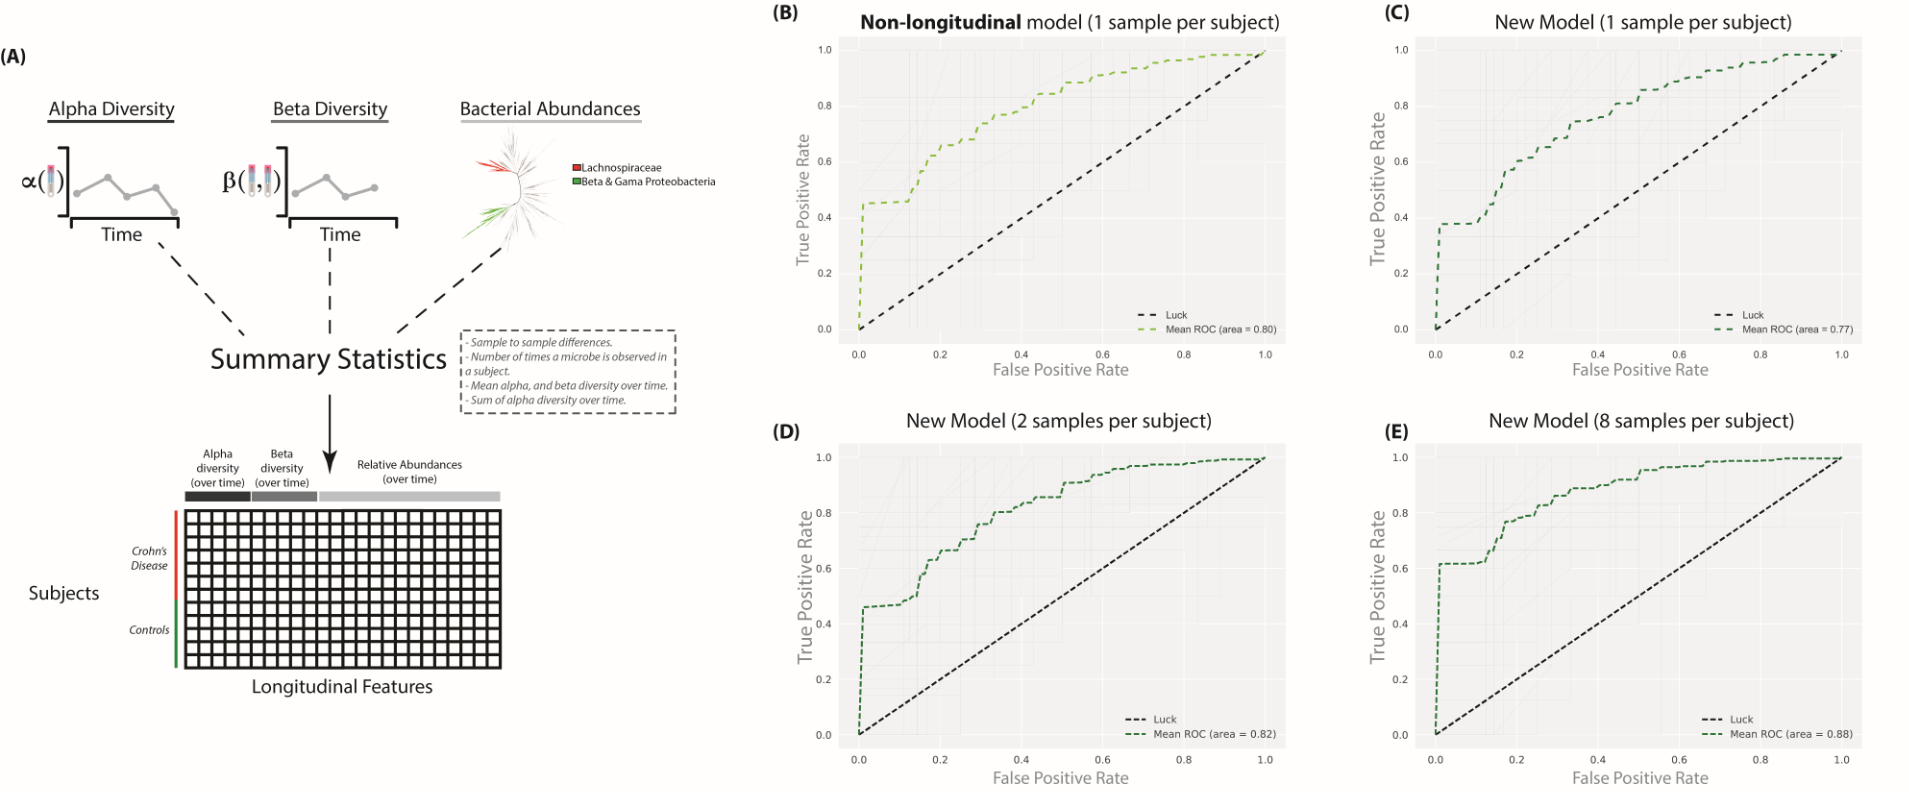
\includegraphics[width=0.95\textheight]{ibd-figures/figure-1}
\caption[Diagram for the model creation, and comparison of four receiver operating characteristic (ROC) curves.]{Diagram for the model creation, and comparison of four receiver operating characteristic (ROC) curves. (A) Diagram describing the origin for the classifying features. (B) ROC curve for a model that relies on relative abundances and one sample per subject (as used in previous publications). (C-D) ROC curve for our new model at 1, 2 and 8 samples per subject. The gray lines represent the performance at each of the 100 iterations. The dotted black diagonal line represents the performance of a classifier that guesses the labels at random.}\label{ibd-fig1}
\end{sidewaysfigure}

\begin{table}[htbp]
\centering
\caption[Performance summary of the classifier at increased samples per subject for this cohort (daily samples) and a previously published cohort.]{Performance summary of the classifier at increased samples per subject for this cohort (daily samples) and a previously published cohort. The area under the curve (AUC) summarizes the performance; closer to 1 is better, of the model trained on the different sample sizes as described by the other columns. The row marked with † represents the performance of a classifier that relies on non-longitudinal relative abundances only.}\label{ibd-table1}
\renewcommand{\arraystretch}{0.8}% Tighter
\begin{tabular}{ccccc}
\toprule
AUC &	Samples per Subject &	Controls &	Crohn's Disease & Sampling\\
\midrule
0.80	&1†&	12 &	19 & \multirow{12}{*}{Daily samples}\\
0.77	&1	& 12 &	19 &\\
0.82	&2	& 12 &	19 &\\
0.85	&3	& 12 &	18 &\\
0.86	&4	& 12 &	18 &\\
0.87	&5	& 12 &	18 &\\
0.87	&6	& 12 &	18 &\\
0.88	&7	& 12 &	18 &\\
0.88	&8	& 12 &	18 &\\
0.87	&9	& 12 &	18 &\\
0.87	&10	& 12 &	17 &\\
0.86	&11	& 12 &	16 &\\
\midrule
0.80	&1†	& 9	& 19 & \multirow{5}{*}{Monthly samples \cite{RN4206}}\\
0.80	&1	& 9	& 19 &\\
0.83	&2	& 9	& 15 &\\
0.86	&3	& 8	& 14 &\\
0.92	&4	& 8	& 12 &\\
\bottomrule
\end{tabular}
\end{table}
\renewcommand{\arraystretch}{1}% Restore original value


Novel analyses aggregating features over time and combining both alpha and beta diversity over time using our intensive daily sampling demonstrates that the main benefits are already obtained by collecting between 3-5 fecal specimens, and no additional benefits are obtained beyond 7 serial samples.  Similar results are found for monthly sampling. These results highlight the importance of treating \gls{cd} as a volatile, time-varying condition, even during clinical remission, but provide hope to clinicians in that a relatively small number of samples yields large additional benefits, facilitating patient compliance. This information can be used to design collection of fecal samples for a large prospective cohort of \gls{cd} patients for longitudinal studies of host-microbial interactions over time.

The methods demonstrated here have not previously been used for microbiome analyses but have been used for other engineering applications, for example in production lines to predict product specification outcomes in a steel manufacturer's facility \cite{RN4216}. We expect the results to generalize in other systems, including other gastrointestinal and hepatic disorders, where dynamic features of the microbiome, host gene expression, or other accessible features can act as indicators of underlying dysbiotic states.

\subsection{Data Processing}

Demultiplexed sequences were filtered using \glspl{qiime} \cite{RN110} default parameters for quality control using (version 1.8.0-dev). To account for the fact that a subset of the sequences were processed using a MiSeq instrument and the rest using a HiSeq instrument, the resulting reads were trimmed to an even length of 99 nucleotides \cite{RN4221, RN4222}. The resulting sequences were clustered using the closed-reference \gls{otu}-picking protocol (utilizing UCLUST as the clustering algorithm \cite{RN81}) against the Greengenes database (release 13\textunderscore 8) \cite{RN165}. Distance matrices were calculated using the UniFrac \cite{RN3770} distance metric. Bimodality tests were performed using Hartigan's dip test \cite{RN4017}. To account for uneven sampling efforts in the samples, the resulting \gls{otu} table was rarefied at 7,400 sequences per sample. The number was selected so the main category of interest (health status of the patient) had a balanced number of classes.

\subsection{Classifier}

To assess the benefits of increased number of samples per subject, we used a Random Forests \cite{RN4205} model and we created the features following these steps. First we randomly selected $N$ samples for each subject.  For this set of $N$ samples, we created features based on alpha diversity, beta diversity and microbial relative abundances. We then split the dataset into training and testing subsets and evaluated the classifier's sensitivity and specificity. Finally, we repeated the selection of $N$ random samples for $M$ iterations, and summarized the results using a \gls{roc} curve and the \gls{auc}. After the $M$ iterations, we increased $N$ by one and repeated the procedure until we reached $N'$. The result is a total of $N'-N$ \gls{roc} curves and \gls{auc} scores (one for each number of samples per subject).

The features are created based on longitudinal patterns of the different data types (alpha diversity, beta diversity and relative abundances). In all cases, we relied on the sample collection date to order the data and measured a series of summary statistics. For alpha diversity and the microbial relative abundances, the per-sample summaries were ordered and treated as vectors. For beta diversity, we considered only the distances between ordered and subsequent timepoints and treated this as a vector. Features were extracted from these vectors as described in the TSFRESH package \cite{RN4216}, for example by counting the number of samples where an individual \gls{otu} is not zero, to include the mean of alpha or beta diversity distances, the mean rate of change of the alpha diversity vector, etc.

In the case of the microbial abundances, we performed a feature selection step using phylofactor \cite{RN4204}. Phylofactorization was performed by maximizing the F-statistic from logistic regression on disease state in patients with \gls{cd}. Over 200 factors were found as significant predictors of \gls{cd} in the terminal ileum, even when controlling for multiple comparisons by a Bonferroni correction. Two factors identified large clades ($>$100 \glspl{otu}) used for feature selection. Factor 3 identified a monophyletic clade of 518 \glspl{otu} in the Lachnospiraceae family which decreases in the terminal ileum of patients with \gls{cd} relative to healthy patients, and factor 26 identified a monophyletic clade containing 737 \glspl{otu} of the \textit{Gammaproteobacteria} and \textit{Betaproteobacteria} classes which increases in relative abundance in the terminal ileum of patients with \gls{cd} relative to healthy patients (Supplementary Figure~1\footnote{\url{https://static-content.springer.com/esm/art\%3A10.1186\%2Fs40168-017-0269-3/MediaObjects/40168_2017_269_MOESM2_ESM.tif}}). The dataset used for feature selection \cite{RN140}, was not used during the training or testing stages of the classifier construction.

Jupyter notebooks and source code describing all the analyses in this paper can be found online\footnote{\url{https://github.com/knightlab-analyses/longitudinal-ibd}}.

\subsection{Methods}

Patients with proven \gls{cd} diagnosed for at least 3 months and in clinical remission were recruited at the University of North Carolina (see Table~\ref{ibd-table1}). Serial stool samples as outlined below were submitted for analysis. Exclusion criteria for entry into the study were active \gls{cd} as defined by a short \gls{cdai} score $>$ 150; fistulizing \gls{cd}, concomitant use of azathioprine (AZA), 6-mercaptopurine (6-MP), methotrexate or anti-TNF agents for less than 3 months; or concomitant use of systemic steroids or budesonide. Steroids or budesonide had to be discontinued at least 8 weeks before inclusion, and local, rectally administered therapies containing 5-ASA (enemas, suppositories) or steroid enemas/foams should have not been used for the previous 4 weeks. Also, \glspl{nsaid} were not allowed as regular treatment, which was defined as use for at least 4 days a week each month. Patients were excluded if they were on antibiotic therapy $\geq$5 days each month or had antibiotic therapy $\geq$5 days in the previous 24 weeks. No probiotics were allowed in the last 24 weeks before inclusion and patients on long-term therapy with narcotics $>$2 days weekly were excluded.  Further subject exclusions were known Hepatitis B, Hepatitis C or PSC or regular, high dose alcohol consumption (more than seven drinks per week). All trial participants were prohibited from consuming specific diets (e.g. Atkins diet, low carbohydrate diet). In the second subset we also included nonaffected family members to collect serial fecal samples.  The requirement for the family subjects was one sibling age $\geq$ 8 years without known \gls{cd} or ulcerative colitis and two living parents without \gls{cd} or ulcerative colitis. The same exclusion criteria for antibiotics, probiotics, narcotics and concomitant diseases as in the main study were applied. 

\begin{table}[htbp]
    \centering
    \caption{Summary of the demographic data of the 19 CD patients.}
    \label{id-tabMethods}
    \begin{tabular}{rrl}
    \toprule
         \multicolumn{2}{r}{Male/Female (n)} &	8 / 11\\
    \midrule
    \multicolumn{2}{r}{Age (years, median; range)} &	31 (15-51)\\
\midrule
\multicolumn{2}{r}{Duration of Crohn's disease (years median; range)} &	9 (0.5-35)\\
\midrule
\multirow{3}{*}{Location of Crohn's disease (n)} & 	Ileal & 5\\
 &   	Ileo-colonic & 10\\
 &     	Colonic	 & 4\\
\midrule
\multicolumn{2}{r}{History of ileocecal resection} &	7\\
\midrule
\multicolumn{2}{r}{History of isolated small intestinal resection} &	2\\
\midrule
\multirow{4}{*}{Concomitant therapies (n)} &        	Steroids & 0\\
&        	Azathioprine/6-MP/methotrexate & 8\\
 &        	anti-TNF agent & 12\\
     &   	5-ASA	 &2\\
\midrule
\multicolumn{2}{r}{\gls{cdai} end of week 2 (mean; SD)} &	63 (51)\\
\midrule
\multicolumn{2}{r}{\gls{cdai} end of week 4 (mean; SD)} &	72 (61)\\
\bottomrule
    \end{tabular}
\end{table}

\subsubsection{Fecal collection}

Stool was collected daily using a swab technique \cite{RN4220}, which enables the study subject to collect stool samples from the toilet paper. Samples were stored on a -20\textdegree C freezer. Fifteen patients collected daily stool for two 2-week periods separated by an interval of 4 weeks, during which no stool was collected.  The short \gls{cdai} was evaluated at entry and at the end of collection period 1 and 2 \cite{RN4006}. The collection periods for the family substudy, which included 4 patients with inactive \gls{cd} with same exclusion criteria as above and 3 unaffected family members of each \gls{cd} patient were two separate 4 weeks periods interrupted by a 3 month collection-free interval.

\subsubsection{DNA Extraction}

Fecal DNA isolation was performed according to the 16S Earth Microbiome Project Protocol \cite{RN164}. Of the 960 samples analyzed, the initial subset (384 samples)  were processed using the Illumina MiSeq platform (150 nucleotide sequences), and for the second subset (576 samples) were processed using the HiSeq platform (100 nucleotide sequences).

\subsubsection{Data Availability}

The sequences have been deposited on EBI and are available under the following accession number ERPXXXX.  In addition, the processed sequences and sample information can be found in the Qiita\footnote{\url{https://qiita.ucsd.edu/study/description/2538}} database under the study identifier 2538.


\subsubsection{Acknowledgments}
We acknowledge grant support by NIH (P01-DK094779), the Crohn's and Colitis Foundation, and the research coordinators of the UNC Multidisciplinary IBD Center at UNC for patient recruitment. Additionally, we thank Gail Ackermann, Jamie Morton and Justin Silverman for their invaluable feedback and discussion provided in the preparation of this manuscript.

\subsubsection{Author Contributions}

Y. V.B. wrote the manuscript, managed the data depositions, interpreted and analyzed the data. A. G. contributed to the manuscript, interpreted and analyzed the data. Z. X. interpreted and analyzed the data. A. W. contributed to the manuscript, interpreted and analyzed the data. H. H., contributed to the manuscript, designed the experiment, interpreted and analyzed the data. R. B. S. wrote the manuscript, designed the experiment, interpreted and analyzed the data. R. K. wrote the manuscript, interpreted, sequenced and analyzed the data. All authors finalized and approved the current version of the manuscript.

\subsubsection{Conflict of interest}
We declare none.

\else
    \section{Janet's IBD paper}\label{section_plane}
    \section{Balfour's IBD paper}\label{section_ibd}
\fi

\chapter{Restoring a lost ecosystem}\label{chapter_fmts}
\glsresetall

\gls{cdi} is a hospital-acquired infection resulting from antibiotic 
administration for an unrelated condition. Paradoxically, the treatment for 
\gls{cdi} is to prescribe more antibiotics. This treatment generally 
translatesto depleted microbial diversity. As a consequence, resources that 
could be consumed by other communities are now available for 
\textit{Clostridium difficile} to thrive on.  More recently \gls{cdi} has been 
treated through the administration of \glspl{fmt}, with a success rate above 
90\% \cite{RN4129}. A \gls{fmt} consists of reintroducing bacteria into the 
\gls{gi} tract of an affected patient. Frequently, after a day, the symptoms of 
\gls{cdi} disappear and the recipients recover. In this chapter, we examine two 
cohorts and focus on the short and long-term changes in the gut microbiota 
after a \gls{fmt}.

In the first cohort, relying on an animated $\beta$-diversity plot (as 
introduced in Section~\ref{section_animations}), we visualize the immediate 
changes in the gut microbiome after a \gls{fmt}. In addition, we also visualize 
the stability of the microbiome after the transplant and note that the only 
point of instability occurs immediately after the \gls{fmt}.

The second cohort is composed of patients suffering from \gls{cdi} and in some 
cases with underlying \gls{ibd}. We find that, while both groups recover from 
the \gls{cdi}, the micro-ecological effects of \gls{fmt} appear to be dampened 
in subjects with underlying \gls{ibd}. Overall, individual phylogenetic 
diversity is lower, and the number of taxa differentially present before and 
after the transplant is also smaller (when compared to the non-\gls{ibd} 
counterparts).

Section~\ref{section_moviefmt} appeared in the journal \textsl{Microbiome, 
2015}.  As the lead analyst in this project, I contributed to the text, 
analyzed and interpreted the data, wrote software used for the analysis, and 
generated the main visuals.  Section~\ref{section_fmt} appered in the journal 
\textsl{Microbiome, 2017}. As the co-lead contributor to this project, I 
co-wrote the text, generated the figures, analyzed, interpreted, and deposited 
the data into a public repository.

\ifdefined\RELEASE
    \glsresetall

\section{Dynamic Changes in Short- and Long-Term Bacterial Composition Following Fecal Microbiota Transplantation for Recurrent \textit{Clostridium difficile} Infection}

\subsubsection{Abstract}

\Gls{fmt} is an effective treatment for recurrent \gls{cdi} that often fails standard antibiotic therapy. Despite its widespread recent use, however, little is known about the stability of the fecal microbiota following \gls{fmt}. Here we report on short- and long-term changes, and provide kinetic visualization of fecal microbiota composition in patients with multiply \gls{rcdi} that were refractory to antibiotic therapy and treated using \gls{fmt}. Fecal samples were collected from four patients before and up to 151 days after \gls{fmt}, with daily collections until 28 days and weekly collections until 84 days post-\gls{fmt}. The composition of fecal bacteria was characterized using high throughput 16S rRNA gene sequence analysis, and compared to microbiota across body sites in the \gls{hmp} database, and visualized in a movie-like, kinetic format. \gls{fmt} resulted in rapid normalization of bacterial fecal sample composition from a markedly dysbiotic state to one representative of normal fecal microbiota.  While the microbiome appeared most similar to the donor implant material one day post-\gls{fmt}, the composition diverged variably at later time points. The donor microbiota composition also varied over time. However, both post-\gls{fmt} and donor samples remained within the larger cloud of fecal microbiota characterized as healthy by the \gls{hmp}. Dynamic behavior is an intrinsic property of normal fecal microbiota, and should be accounted for in comparing microbial communities among normal individuals and those with disease states.  This also suggests that more frequent sample analyses are needed in order to properly assess success of \gls{fmt} procedures.

\subsection{Introduction}

\Gls{fmt} has emerged in recent years as a highly effective treatment for refractory \gls{cdi} that cannot be cured with antibiotics alone \cite{RN65}. The procedure leads to prompt engraftment of donor microbiota, attainment of donor-like bacterial diversity, and normalization of the overall microbial community structure \cite{RN53moviefmt, RN30, RN66, RN31, RN36, RN4129, RN1}. However, existing data characterizing long-term stability of engrafted microbiota are limited. One recent study suggests the microbiota of patients after \gls{fmt} may not fully recover until 16 weeks after the procedure \cite{RN35moviefmt}. This type of analysis, however, is complicated by the fact that the microbial communities are intrinsically dynamic, and affected by daily fluctuations in the host's diet, activities, and health \cite{RN4235, RN67, RN4195}. In addition, multiple fixed host factors, such as different states of immune competence, genetics, or gastrointestinal anatomy, likely also affect the composition, stability, or resilience of colonic microbiota \cite{RN41, RN74, RN3801, RN73, RN71}. Therefore, it is unclear whether divergence in post-\gls{fmt} microbiota from that of donor implant material represents continued recovery, or whether these temporal changes are a general characteristic of host-associated gut microbiota in a changing host environment.

Here we describe both short- and long-term dynamic changes of fecal bacterial composition in four patients following \gls{fmt}. All patients received microbiota from the same pre-qualified donor according to the standardized \gls{fmt} protocol we described previously \cite{RN45}. Three patients received freshly prepared microbiota and one patient received microbiota that had previously been frozen. We compared pre- and post-\gls{fmt} fecal microbial communities from these patients, as well as pre-\gls{fmt} communities from 10 additional patients with multiply \gls{rcdi}, to the sequences of normal subjects described in the Human Microbiome Project \cite{RN75}.  In addition, we compared temporal changes in fecal bacterial composition in recipients following \gls{fmt} to temporal changes observed within samples from the donor.

\subsection{Materials and Methods}
\subsubsection{Patients and donors}
All patients suffered from multiply \gls{rcdi} refractory to standard antibiotic therapies. A single standard donor was used in the preparation of all fecal microbiota material as described previously \cite{RN45}. The Institutional Review Board at the University of Minnesota approved prospective collection of fecal specimens and their analysis. All patients satisfied the inclusion criteria for the \gls{fmt} within our program, which included at least two spontaneous recurrences of \gls{cdi} within a month of discontinuation of antibiotics and failure of at least one advanced antibiotic regimen such as a vancomycin pulse/taper protocol or vancomycin treatment followed by administration of rifaximin or fidaxomicin for 2-3 weeks.  The specific clinical characteristics of patients involved in this study are summarized in Supplementary Table~1\footnote{\url{https://static-content.springer.com/esm/art\%3A10.1186\%2Fs40168-015-0070-0/MediaObjects/40168_2015_70_MOESM3_ESM.xlsx}}.  

\subsubsection{Fecal microbiota transplantation}
\Gls{fmt} was done using a standardized preparation of concentrated fresh or frozen fecal bacteria via colonoscopy as previously described \cite{RN45}. All patents were treated with oral vancomycin, 125 mg four times daily, until two days prior to the procedure \cite{RN45}. The day before the procedure, patients received a polyethylene glycol-based colonoscopy prep (GoLYTELY\textsuperscript{\textregistered} or MoviPrep\textsuperscript{\textregistered}) to remove residual antibiotics and fecal material. Donor fecal microbiota was placed into the terminal ileum and/or cecum via the biopsy channel of the colonoscope. A total of 17 donor samples from the same individual were used in these studies.  The CD1-CD4 donor samples were given to patients CD1-CD4, respectively. Patients CD1, CD3, and CD4 received freshly prepared fecal microbiota, while patient CD2 received a previously frozen preparation of fecal microbiota, all from the same standardized, anonymous donor.

\subsubsection{Sample collection}
Fecal samples were collected at home by the patients using swabs to sample feces deposited into a toilet hat immediately after production, and stored frozen at approximately -20\textdegree C. Samples were subsequently transferred to the laboratory and stored at -80\textdegree C until used. Donor samples for DNA extraction were collected during processing of material for \gls{fmt}, and stored frozen at       -80\textdegree C until used. Samples from patients CD1- 4 were obtained prior to \gls{fmt} and between 1 to 151 days post-\gls{fmt}, with daily collection until day 28, and weekly collection until day 84. Fecal material prior to \gls{fmt} was obtained from patients CD5-CD14.

\subsubsection{DNA extraction}
DNA was extracted from donor and recipients' pre- and post-\gls{fmt} fecal samples using MOBIO PowerSoil DNA extraction kits (MOBIO, Carlsbad, CA), according to the manufacturer's instructions. Fecal DNA concentrations were measured using a QuBit DNA quantification system (Invitrogen, Carlsbad, CA).

\subsubsection{PCR amplification}
Extracted DNA was amplified using the EMP standard protocols\footnote{\url{http://www.earthmicrobiome.org/}} following the recommendations of Caporaso et al. \cite{RN4221}. Briefly, F515/R806 primers were used, with 12-base Golay codes introduced on the 806 end to provide unique sample indices. Cycling and annealing conditions were as previously described \cite{RN4221}.

\subsubsection{DNA sequencing}
DNA sequencing was performed as previously described \cite{RN4221} on an Illumina MiSeq platform using 2 x 150 bp paired-end reads and the Illumina v3 reagent chemistry. 

\subsubsection{Sequence processing and analysis}
Sequence data was processed and analyzed using \gls{qiime} \cite{RN4052} according to the Illumina demultiplexing and processing protocol \cite{RN4221} and current quality-filtering recommendations \cite{RN4160}, using the 1.8.0 pipeline and the default parameters in split\textunderscore libraries\textunderscore fastq.py. After quality control and demultiplexing, we picked close references at 97\% similarity against the 97\% similarity Greengenes database \cite{RN176} version 13\textunderscore 8. All further analyses were performed at a rarefied depth of 5,000 reads/sample.  EMPeror \cite{RN79} was used for data visualization of BIOM-format \cite{RN3811} \gls{otu} tables. \gls{otu} analyses were performed by clustering at the 97\% level with UCLUST \cite{RN81}, and data were integrated with the \gls{hmp} dataset according to the protocols used for similar previous meta-analyses \cite{RN3801, RN82}. Sequences were analyzed by using both weighted and unweighted UniFrac \cite{RN133}, followed by principal coordinate analysis \cite{RN3740}. Data were visualized using Phinch.  The Phinch program provides an easy-to-use, browser-based, platform to visualize contingency tables along with their sample metadata (Bik et al., manuscript in preparation\footnote{\url{https://github.com/PitchInteractiveInc/Phinch}}).

\subsubsection{Analysis of microbiome stability and centrality}
For each set of post-transplant patient samples we assessed the similarity of that set to the set of reference samples from the donor (2,000 reads/sample). To reduce noise and compare patient samples along only relevant dimensions in UniFrac distance space, we applied \gls{pcoa} to the unweighted UniFrac distance matrix containing only the post-transplant and donor samples for that donor-patient pair, then recalculated the distances using only the first n principal coordinates axes required to explain at least 80\% of the variation in the distance matrix. An 80\% cutoff was chosen to balance bias and overfitting. Distances were recalculated using Euclidean distances between points in \gls{pcoa} space in order to convert \gls{pcoa} coordinates to a distance matrix. The empirical p-values for the `normality' were obtained by comparing the mean distance between patient and donor samples to the histogram of within-donor distances (generated using all samples from a given donor by enumerating the pairwise distance between those samples). The empirical p-values for the `dynamic range' (stability) were obtained by comparing the mean distance within patient samples to the histogram of within-donor distances. These analyses were also performed using alternative parameters including, weighted UniFrac, Jensen-Shannon, root Jensen-Shannon, and Bray-Curtis.


\subsection{Results}
\subsubsection{Bacterial composition of fecal samples from patients with R-CDI becomes healthy and donor-like following FMT}

Four patients (CD1-CD4) with \gls{rcdi} were treated with \gls{fmt} using material obtained from a single donor but from different time points, and fecal samples were collected from these patients before and after the procedure as well as from the donor at times of donation. Bacterial communities from these fecal samples were characterized by sequencing the V4 region of the 16S rRNA gene. Following trimming and quality filtering from a total of 12,536,492 sequences, we randomly subsampled to 5,000 sequences/sample in order to normalize read depth across all samples. All further analyses were performed using this rarefied read depth.

To better understand changes in bacterial communities following \gls{fmt}, we compared the bacterial composition of patient fecal samples to those of microbial communities from various body sites from the 252 healthy individuals characterized in the \gls{hmp} \cite{RN75} (Figure~\ref{moviefmt-fig1}) using unweighted UniFrac \cite{RN133} followed by \gls{pcoa} \cite{RN4052} (see Movie Supplement\footnote{\url{https://static-content.springer.com/esm/art\%3A10.1186\%2Fs40168-015-0070-0/MediaObjects/40168_2015_70_MOESM1_ESM.mp4}}). The composition of pre-\gls{fmt} fecal samples from patients CD1-CD4 and 10 additional patients with \gls{rcdi} was distinct from both fecal samples from healthy individuals and microbial communities at other body sites, including mouth, vagina, and skin, demonstrating severe alterations in pre-\gls{fmt} communities compared to healthy fecal communities as has been previously shown \cite{RN30, RN4129}. In contrast, microbial communities from the donor fell within the range of healthy fecal samples. Using an animated visualization of \gls{fmt}-associated changes in patients' fecal microbial communities, we observed rapid and dramatic shifts after \gls{fmt} towards the communities found in the feces of healthy individuals and of the original donor (see Movie Supplement\footnote{\label{supmoviefmt}\url{https://static-content.springer.com/esm/art\%3A10.1186\%2Fs40168-015-0070-0/MediaObjects/40168_2015_70_MOESM1_ESM.mp4}}).

\begin{figure}[htbp]
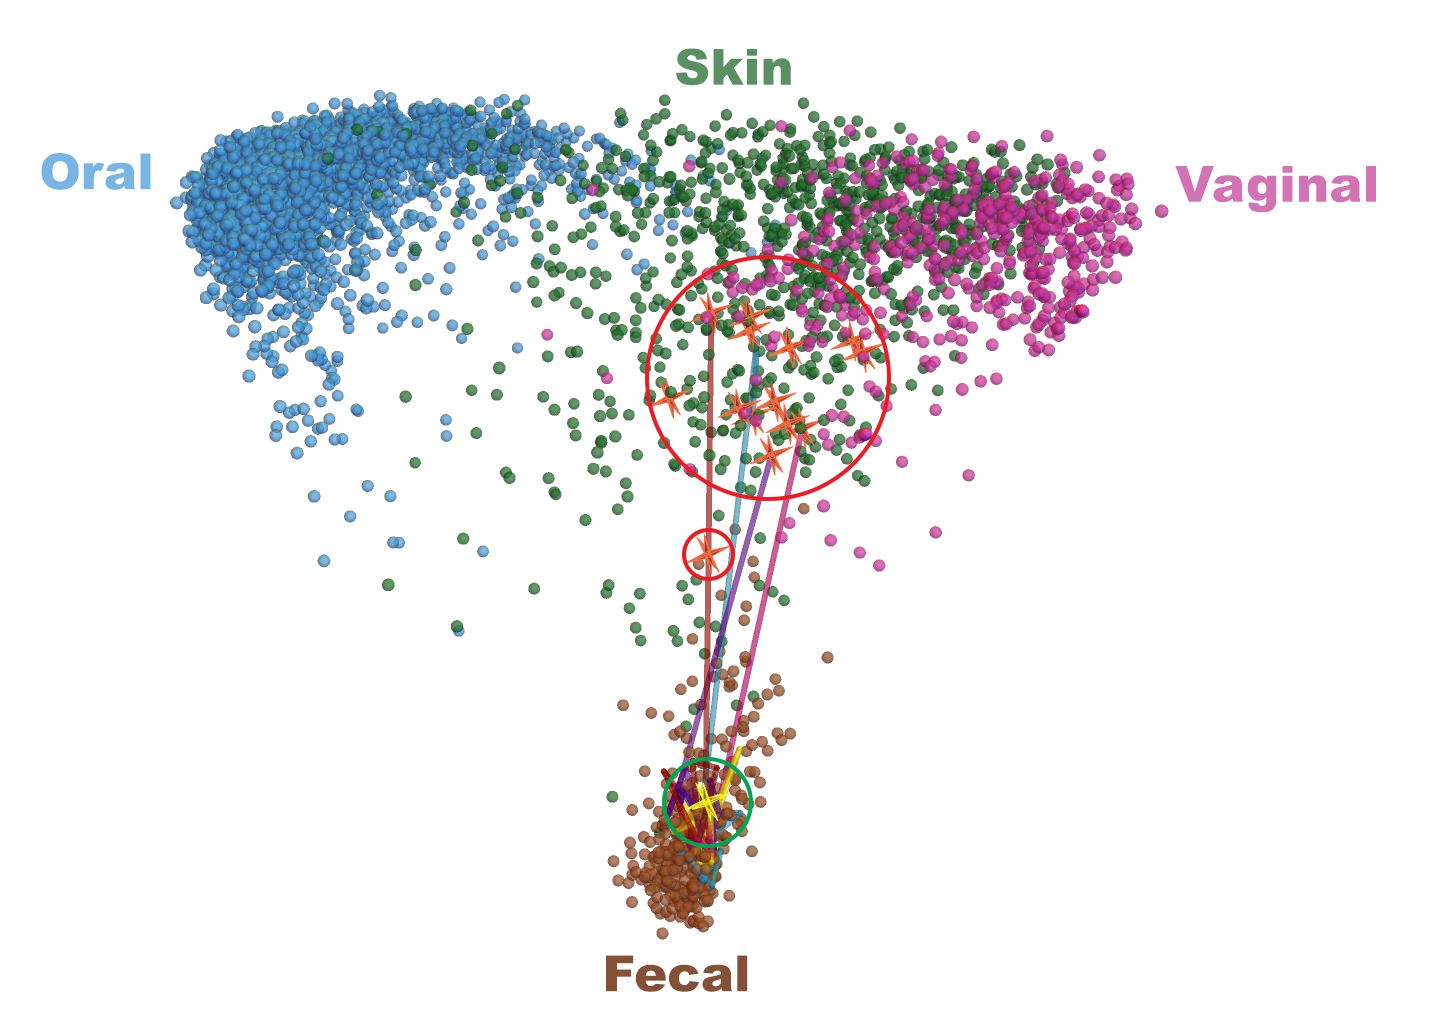
\includegraphics[width=\columnwidth]{moviefmt-figures/figure-1}
\caption[Fecal bacterial communities of recurrent CDI patients shift towards HMP fecal bacterial communities after FMT.]{Fecal bacterial communities of recurrent CDI patients shift towards HMP fecal bacterial communities after FMT. Red circles = pre-FMT patient samples; green circle = post-FMT patient samples; blue line = trajectory of patient fecal communities after FMT.}
\label{moviefmt-fig1}
\end{figure}

\subsubsection{Fecal microbial communities remain dynamic following FMT}
To more closely examine temporal changes in recipient fecal samples following \gls{fmt}, we analyzed fecal microbial communities from patients CD1-CD4 and donor, as well as from 10 additional donor samples, using weighted and unweighted UniFrac \cite{RN83} followed by \gls{pcoa} \cite{RN4052}. This analysis demonstrated that fecal bacterial communities continued to undergo compositional fluctuation following \gls{fmt} (Figure~\ref{moviefmt-fig2}A and S1; individuals \glspl{otu} listed in Table S1).

\begin{sidewaysfigure}[htbp]
\includegraphics[width=\textheight]{moviefmt-figures/figure-2}
\caption[Microbial communities shift following FMT.]{Microbial communities shift following FMT. A) Unweighted (left) and weighted (right) UniFrac analyses followed by principal component analysis of bacterial communities of recurrent CDI patient fecal samples before (red) and after FMT and donor samples (blue). B) Weighted UniFrac analysis followed by principal component analysis of bacterial communities of patients before (red) and after FMT versus HMP fecal communities (purple). PC: principal component. Percentages represent percent variability explained by each principal component. Se key at right for colors associated with samples before FMT (Pre-FMT), from HMP and donor, and from patients after FMT (CD1-CD4).}
\label{moviefmt-fig2}
\end{sidewaysfigure}

To determine whether this dynamic range of post-\gls{fmt} microbial composition fits within the range seen across healthy individuals, we also compared communities in our samples to those in the \gls{hmp} via weighted UniFrac and \gls{pcoa} (Figure~\ref{moviefmt-fig2}B). Again, fecal microbial communities prior to \gls{fmt} were highly distinct from healthy fecal microbial communities, and following the procedure these communities more closely resembled those of healthy individuals. Similar to the comparison with donor communities above, fecal microbial communities of \gls{rcdi} patients following \gls{fmt} shifted within the cluster of communities from healthy individuals.

\subsubsection{Rapid and substantial changes to \textit{Enterobacteriales} in feces following FMT}

While overall fecal microbial communities were dramatically altered following \gls{fmt}, we also examined the effects of the procedure on the abundance and dynamics of individual bacterial taxa within the four original \gls{cdi} patients. As shown previously \cite{RN53moviefmt, RN30, RN66, RN31, RN36, RN4129, RN1}, the relative abundance of bacterial phyla in patient fecal samples shifted substantially following \gls{fmt}, with relative decreases in \textit{Proteobacteria} and relative increases in \textit{Bacteroidetes} and \textit{Firmicutes} (Figure~\ref{moviefmt-fig3}). These \textit{Proteobacteria} are primarily the order \textit{Enterobacteriales}, which were also substantially decreased in relative abundance following \gls{fmt} (Figure~\ref{moviefmt-fig4}A).

\begin{sidewaysfigure}[htbp]
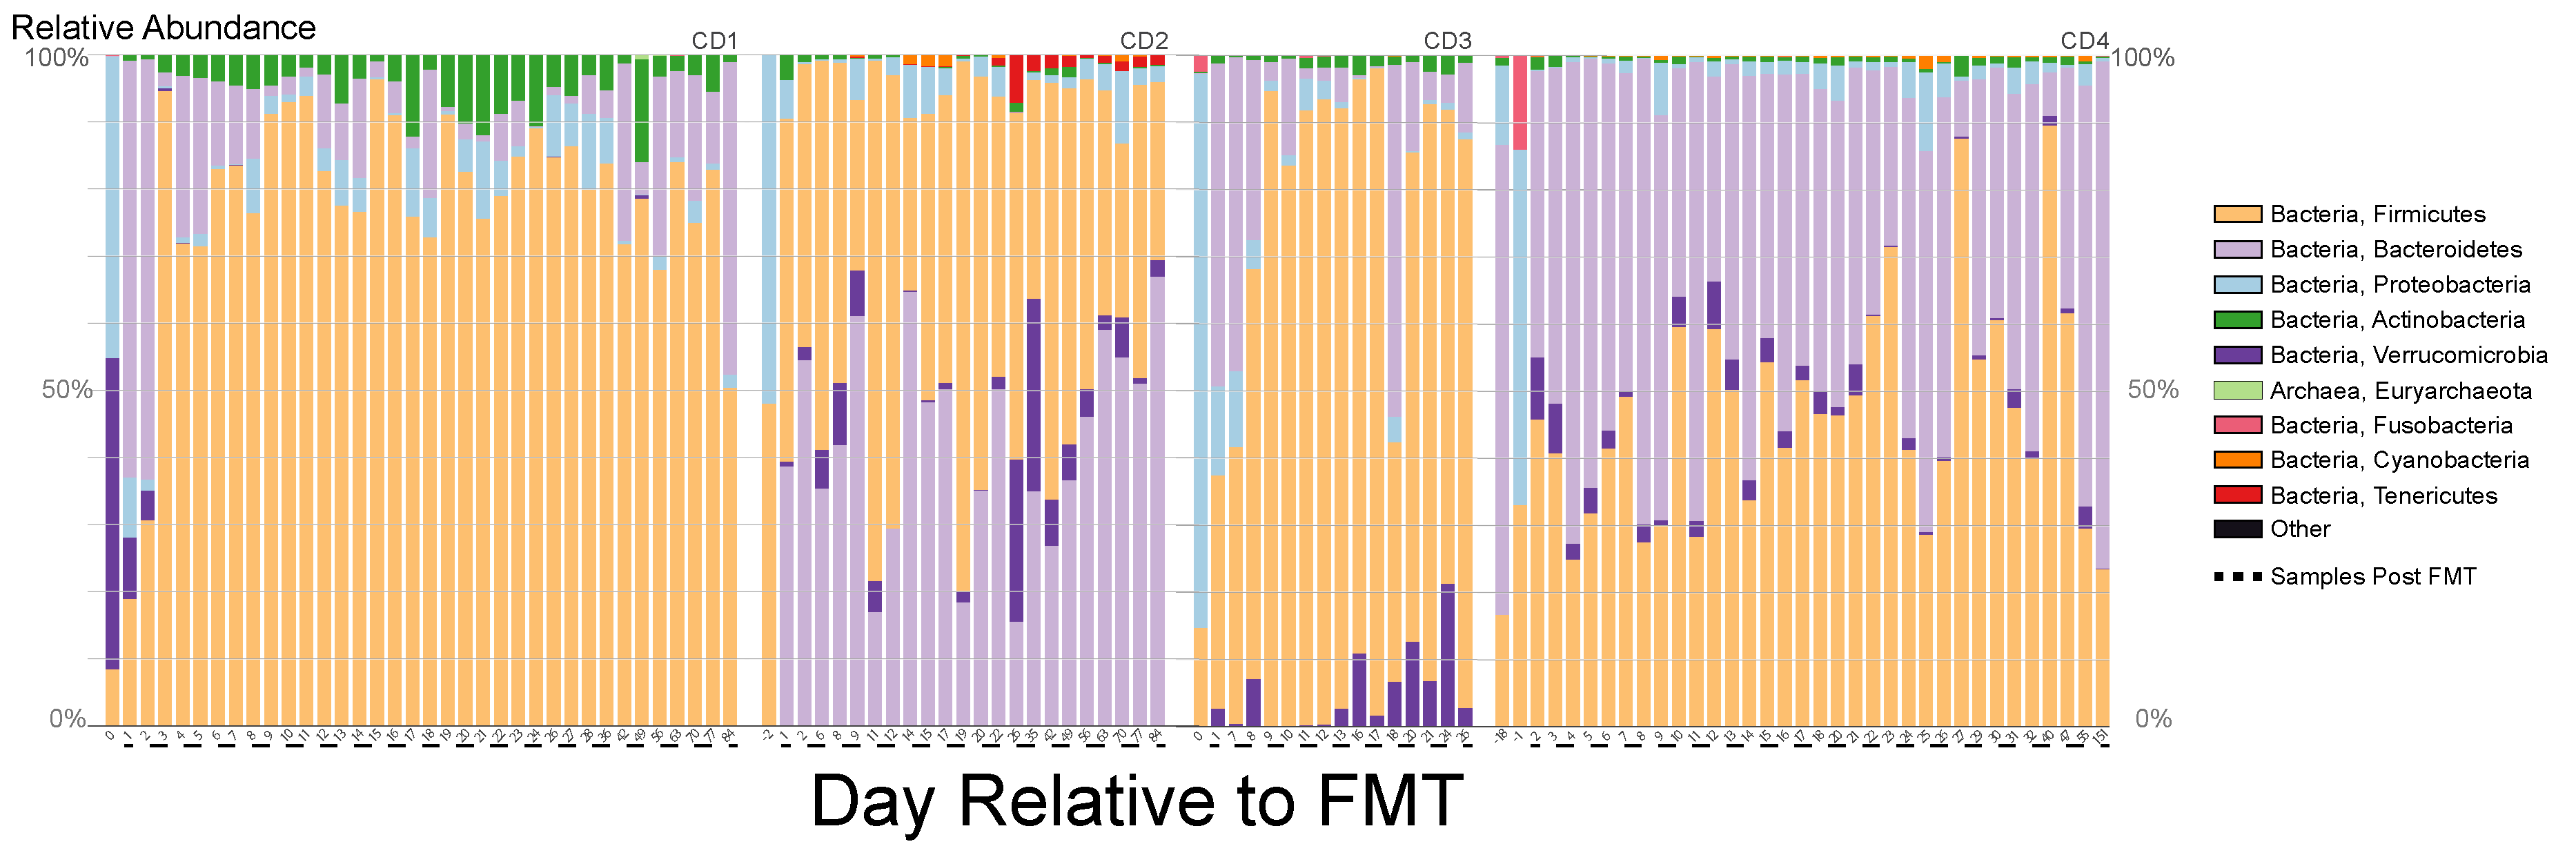
\includegraphics[width=\textheight]{moviefmt-figures/figure-3}
\caption[Changes in fecal microbial communities after FMT.]{Changes in fecal microbial communities after FMT. Relative abundance of sequences classified to the level of bacterial phyla before and after FMT in patient fecal samples. Samples after FMT indicated with dashed line. See key at right.}
\label{moviefmt-fig3}
\end{sidewaysfigure}

We focused on these changes by examining the relative abundance of \textit{Enterobacteriales} alone in each patient before and after \gls{fmt}. The relative abundance of this taxon ranged from 44 to 82\% in all four patient samples prior to \gls{fmt}, and rapidly dropped to undetectable levels within one week after the procedure. Moreover, abundance of this taxon remained low at 26 days after \gls{fmt}, the latest time point shared by all four patients (Figure~\ref{moviefmt-fig4}A), although other members of the \textit{Proteobacteria} remain detectable if decreased in relative abundance (Figure~\ref{moviefmt-fig3}). In addition, we generated individual value control charts based on the average abundance of this taxon in \gls{rcdi} patients. Compared to relative abundance, these control charts displayed the expected variation of the abundance of \textit{Enterobacteriales} in these fecal samples. In all patients, the abundance of \textit{Enterobacteriales} was above the expected variation (i.e. more than three standard deviations above the mean relative abundance [\gls{ucl}] of this order across all samples) prior to \gls{fmt}, and rapidly fell below the upper control limit within 1-2 days after the procedure (Fig~\ref{moviefmt-fig4}B). These results suggest that the relative abundance of \textit{Enterobacteriales} significantly decreased in all patients soon after \gls{fmt} to levels similar to donor samples, and remained within a statistically expected range for the duration of sample collection (up to 151 days post-\gls{fmt}).

\begin{sidewaysfigure}[htbp]
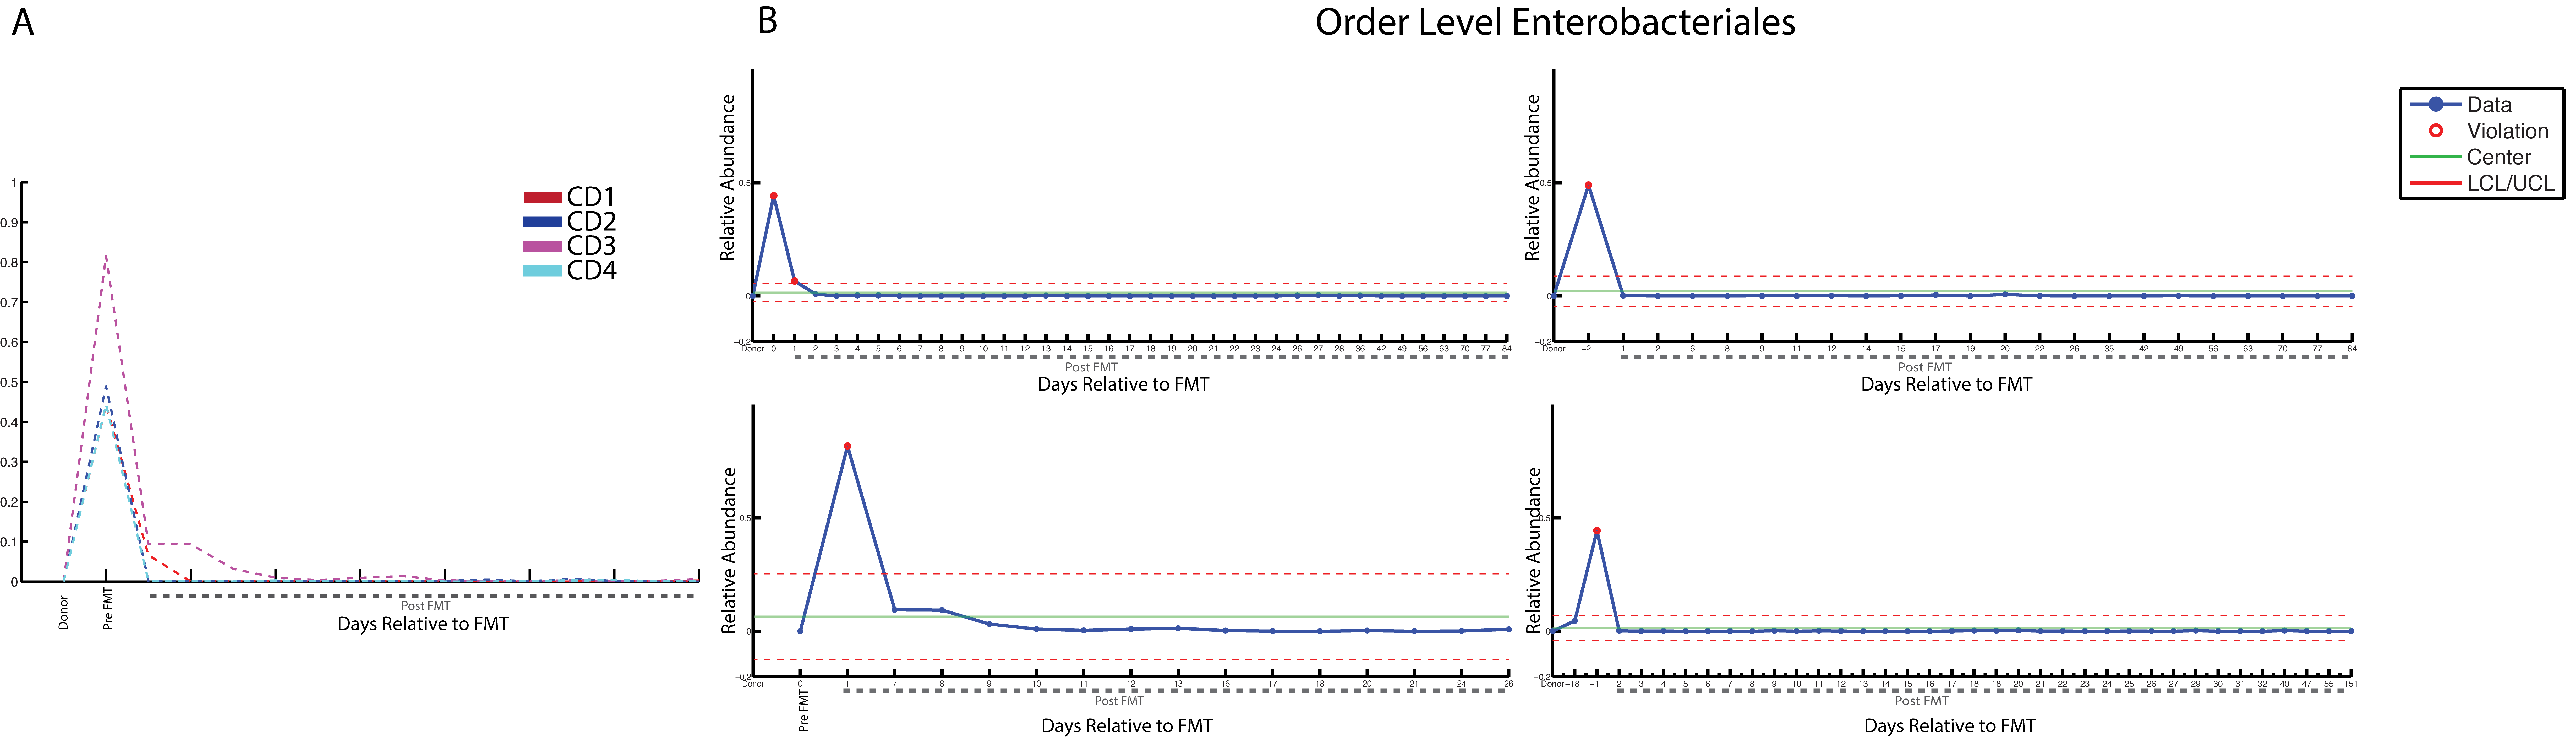
\includegraphics[width=\textheight]{moviefmt-figures/figure-4-small}
\caption[Changes in the order \textit{Enterobacteriales} after FMT.]{Changes in the order \textit{Enterobacteriales} after FMT. A) Relative abundance of \textit{Enterobacteriales} in donor and patient samples before and after FMT in samples common across all patients. B) Control charts of relative abundance of \textit{Enterobacteriales} in donor (leftmost sample) and patient samples before and after FMT. Top left: patient CD1, top right: patient CD2, bottom left: patient CD3, bottom right: patient CD4. LCL: lower control limit; UCL: upper control limit; Center: mean relative abundance in all samples. LCL and UCL represent three standard deviations in relative abundance below and above the mean, respectively. Dashed lines indicate samples after FMT.}
\label{moviefmt-fig4}
\end{sidewaysfigure}

\subsubsection{Post-FMT communities are initially similar to donor samples but can later diverge}

Next, we compared fecal microbial communities within each patient over time to that of the initial donor sample. We generated heat maps based on Pearson correlations between every sample within a given patient set, including respective donor samples and samples from 10 additional pre-\gls{fmt} patients (Figure~\ref{moviefmt-fig5}A). This analysis revealed that while microbiota in samples from patients after \gls{fmt} quickly became similar to microbiota in donor samples, the similarity of samples taken at later time points after \gls{fmt} fluctuated.

\begin{sidewaysfigure}[htbp]
\includegraphics[width=\textheight]{moviefmt-figures/figure-5-small}
\caption[Pearson and Spearman correlations between fecal communities before and after FMT.]{Pearson and Spearman correlations between fecal communities before and after FMT. A) Heat map of Pearson correlation values between each sample within each patient set, corresponding donor, and 10 additional pre-FMT patient samples (far right). B) Pearson correlation values between donor sample and each patient sample. C) Spearman correlations between donor sample and each patient sample. D) Heat maps of Pearson (i) and Spearman (ii) correlation values between earliest donor sample and eleven subsequent samples; days represent collection time of each sample versus earliest donor sample. CD1-4: patients 1-4. Dashed lines indicate samples after FMT.}
\label{moviefmt-fig5}
\end{sidewaysfigure}

To further investigate how fecal microbial communities in these patients correlate to donor communities, we examined Pearson and Spearman correlations between donor and patient samples, which were common to each patient (pre-\gls{fmt} samples and those up to 26 days post-\gls{fmt}; Figure 5B and C and Figure S2). While fecal microbial communities from patients before \gls{fmt} were highly distinct from those in the donor, fecal microbial communities from samples one day after the procedure were highly correlated to donor communities via both Pearson and Spearman analyses in all patients. After the initial time point after \gls{fmt}, the Pearson correlation values of patient to donor samples were highly variable within and across patients, although Spearman correlations remained high for three patients. To examine whether this variation is similar in healthy individuals, we determined Pearson and Spearman correlations within the four donor samples used in \gls{fmt}, as well as eight additional donor samples from the same individual as a control. Results of this analysis revealed that donor microbiota also changed over time (Figure 5D). These findings suggested that the level of variability seen across patient post-\gls{fmt} fecal microbial communities was within the range of normal microbiota behavior in a healthy individual.

\subsubsection{Normalization and dynamic range of post-FMT patient fecal microbial communities are similar to donor communities}

Because of the observed variability in later post-\gls{fmt} patient fecal communities relative to single donor communities, we compared the communities of these patient samples to an expanded set of 17 samples taken from the same donor. We generated two metrics to evaluate the relationships between these communities: normalization and dynamic range (stability). Normalization refers to the mean between-sample distance for each set of patient samples versus the set of donor samples, while dynamic range is the mean distance between each sample within a single patient set. Effectively, the normality of a post-\gls{fmt} patient sample set is a measure of how similar it is to the donor (healthy) sample set, while dynamic range is a measure of variability within a given patient sample set. We found that neither the normalization nor the dynamic range of any post-\gls{fmt} patient sample set was significantly different than the donor set following analysis using unweighted UniFrac  (Table~\ref{moviefmt-tab1}). This suggested that although fecal microbial communities of patients post-\gls{fmt} do not remain identical to the donor, they nonetheless fall within expected parameters relative to the healthy donor. Similar results were obtained when these analyses were repeated with other parameters, including weighted UniFrac, Jensen-Shannon,  and root Jensen-Shannon, and Bray-Curtis (data not shown).

\begin{table}[hbtp]
    \caption{P-values of normalization and dynamic range of patient samples sets versus donor set.}
    \label{moviefmt-tab1}
    \centering
    \begin{tabular}{ccccc}
    \toprule
        \textbf{Patient} &    CD1 &    CD2 &    CD3 & CD4\\
    \midrule
        \textbf{Normalization} &    0.154 & 0.429 &    0.165 & 0.484\\
        \textbf{Dynamic Range} &    0.484 & 0.429 &    0.308 & 0.473\\
    \bottomrule
    \end{tabular}
    
\end{table}

\subsection{Discussion}
It is now well understood that the fecal microbiota change substantially following \gls{fmt}, typically shifting to fecal microbial communities more similar to those of the donor after transplant \cite{RN53moviefmt, RN30, RN66, RN31, RN36, RN4129, RN1}. Here we show that these communities shift away from a dysbiotic state towards a composition that is representative of fecal microbial communities from hundreds of healthy individuals, collected in the \gls{hmp} \cite{RN75}. Similarly to previous studies \cite{RN53moviefmt, RN30, RN31, RN4129, RN1}, the dysbiotic state in these patients with multiply \gls{rcdi} is characterized by a large expansion of \textit{Proteobacteria} (primarily members of the order Enterobact\textit{}eriales, which contains the family \textit{Enterobacteriaceae}), and \gls{fmt} is associated with reemergence of dominance by members of the \textit{Bacteroidetes} and \textit{Firmicutes} phyla.

Analysis of multiple donor and post-\gls{fmt} samples demonstrates the dynamic behavior of fecal microbial communities over time. Both donor and recipient samples are characterized by highly dynamic shifts that nonetheless remain within the compositional range of normal fecal microbiota. This observation is consistent with known rapid responsiveness of the fecal microbiome to environmental inputs, such as dietary variations \cite{RN4235}, and drifts in microbiota composition over time in healthy individuals \cite{RN84}. 

The dynamic nature of intestinal microbiota is an intrinsic property, which should be taken into account when considering how therapeutic interventions, including \gls{fmt}, impact its composition over time. In long-term post-\gls{fmt} follow-up, Song and colleagues also noted dynamic changes in the fecal microbiome of \gls{rcdi} patients up to 16 weeks post-\gls{fmt} \cite{RN35moviefmt}. These investigators concluded that the fecal microbiome of post-\gls{fmt} patients did not fully recover over this time, despite clinical recovery. Indeed, we observed divergence of microbiome in some of the patients away from the original implanted material over time. However, analysis of multiple donor samples showed that this movement is within the same dynamic range observed in the donor's fecal microbiome. We therefore conclude that the dynamic behavior of microbiota needs to be taken into account in making comparisons between individuals, and should become an integral part of analysis of the success of \gls{fmt}.

Three of the recipients in this study received freshly prepared microbiota, while one received frozen/thawed preparation. Use of frozen microbiota preparations is increasing in clinical practice \cite{RN26}, and its equivalency has not been rigorously established in randomized clinical trials. The ability to store microbiota allows the most up-to-date testing of the donor and fecal material for infectious pathogens, as some of the current tests may take several weeks to complete. Therefore, ability to preserve donor microbiota long-term is critical for its development as a therapeutic agent in clinical practice. Our results here, although limited in the number of patients, demonstrate indistinguishable behavior of fresh and frozen/thawed microbiota preparation.

The patients in this study did not have any significant gastrointestinal co-morbidities. However, a significant proportion of patients with \gls{rcdi} have underlying inflammatory bowel disease, take potent immunosuppressive medications, or have multiple other medical problems \cite{RN45, RN85}. The importance of these host factors in contributing to microbiota behavior is currently unknown, but is a subject of great interest \cite{RN87}. Understanding these influences will require analysis of multiple samples. Recently, Fuentes and colleagues \cite{RN53moviefmt} reported that some specific microbial groups and interactive networks are likely to be very important for the maintenance of microbiota in healthy individuals. However, although there is a great deal of effort focused on discovery of compositional differences in microbiota between normal subjects and individuals with different gastrointestinal and medical conditions, the dynamic behavior of fecal microbiota constitutes another dimension that may distinguish these cases. Thus, predictors of stable or dysbiotic intestinal microflora may also change over time. Further detailed studies of dynamic behavior of post-\gls{fmt} microbiota may improve our understanding of causal connections between microbial communities and different disease states.   

\subsubsection{Acknowledgements}

This research was supported, in part, by NIH Grant R21AI091907 (to AK and MJS). ARW was supported by a Doctoral Dissertation Fellowship from the University of Minnesota Graduate School and by the Dennis W. Watson Fellowship in Microbiology. Work done in the Knight lab was funded by the NIH, Crohn's \& Colitis Foundation of America, and the HHMI.  

    \glsresetall

\section{Changes in Microbial Ecology after Fecal Microbiota Transplantation for recurrent \textit{C. difficile} Infection Affected by Underlying Inflammatory Bowel Disease}

\subsubsection{Background}
Gut microbiota play a key role in maintaining homeostasis in the human gut. Alterations in the gut microbial ecosystem predispose to \gls{cdi}, and gut inflammatory disorders such as \gls{ibd}. \Gls{fmt} from a healthy donor can restore gut microbial diversity and pathogen colonization resistance; consequently it is now being investigated for its ability to improve inflammatory gut conditions such as \gls{ibd}.  In this study, we investigated changes in gut microbiota following \gls{fmt} in 38 patients with \gls{cdi} with or without underlying \gls{ibd}. 

\subsubsection{Results}
There was a significant change in gut microbial composition towards the donor microbiota, and an overall increase in microbial diversity consistent with previous studies after \gls{fmt}. \gls{fmt} was successful in treating \gls{cdi} using a diverse set of donors, and varying degrees of donor stool engraftment suggesting that donor type and degree of engraftment are not drivers of a successful \gls{fmt} treatment of \gls{cdi}. However, patients with underlying \gls{ibd} experienced an increased number of \gls{cdi} relapses (during a 24-month follow-up), and a decreased growth of new taxa, as compared to the subjects without \gls{ibd}, note that the test used presents some limitations in sample size and statistical assumptions (see methods). Moreover, the need for \gls{ibd} therapy did not change following \gls{fmt}. These results underscore the importance of the existing gut microbial landscape as a decisive factor to successfully treat \gls{cdi}, and potentially for improvement of the underlying pathophysiology in \gls{ibd}. 

\subsubsection{Conclusions}
\Gls{fmt} leads to a significant change in microbial diversity in patients with recurrent \gls{cdi} and complete resolution of symptoms. Stool donor type (related or unrelated) and degree of engraftment are not key for successful treatment of \gls{cdi} by \gls{fmt}. However, \gls{cdi} patients with \gls{ibd} have higher proportion of the original community after \gls{fmt} and lack of improvement of their \gls{ibd} symptoms and increased episodes of \gls{cdi} on long-term follow-up.

\subsubsection{Keywords}
Fecal microbiota transplantation, microbiome, Clostridium difficile infection, inflammatory bowel disease

\subsection{Background}

Gut microbiota play a key role in maintaining homeostatic host functions and deleterious shifts in the gut microbial ecosystem, often referred to as dysbiosis, are associated with \gls{cdi}, \gls{ibd} and other systemic inflammatory conditions \cite{RN1477}. A diverse gut microbial community confers colonization resistance against pathogens such as \textit{C. difficile}, and disruption of a diverse community structure from antibiotics, comorbidities, altered gastrointestinal transit or other risk factors can lead to pathogen colonization and infection \cite{RN1480}.

With increasing incidence of community and hospital acquired \gls{cdi}, high rates of recurrent \gls{cdi} (estimated 20-30\% after a first and 50-60\% after a third infection), high mortality (~29,000 deaths annually) in the United States, and an urgent need for newer non-antibiotic therapies has led to the emergence of microbiome based therapies \cite{RN1478}. \Gls{fmt} in \gls{cdi} patients restores phylogenetic diversity to levels more typical of a healthy person, with response rates $>$85\% by enema, oral capsule or endoscopic delivery modes \cite{RN1484, RN1479, RN1481}. A recent study suggests significantly lower response of \gls{cdi} to \gls{fmt} in patients with underlying \gls{ibd} \cite{RN1497}. We have also previously described a higher rate of recurrence of \gls{cdi} following \gls{fmt} in patients with \gls{cdi} and underlying \gls{ibd} \cite{RN1498}. It remains unclear if changes in gut microbial ecology play a role in long-term success of \gls{fmt} in these patients.

\Gls{fmt} has not shown consistent success in treating other diseases associated with microbial dysbiosis such as \gls{ibd}. Three clinical trials to treat \gls{uc} with \gls{fmt} have shown conflicting results and one highlighted the potential role of specific gut microbial members in donor stool in determining success after \gls{fmt} in \glspl{uc} \cite{RN3982, RN1019, RN1483}.  The underlying host or donor factors that may be important for success of \gls{fmt} in treatment of \gls{ibd} remain unclear.

In this study, we assessed the effect of donor type (standard donor versus related donor) and changes in gut microbial ecology on response to \gls{fmt} in \gls{rcdi} with and without underlying \gls{ibd} as well as clinical response to \gls{fmt}. 

\subsection{Methods}
\subsubsection{Patient selection}
Patients undergoing \gls{fmt} for \gls{rcdi} were prospectively recruited in this study. Informed consent was obtained to collect clinical data and stool samples. Data collected included demographics, clinical history, \gls{cdi} treatment history, comorbid conditions and response to \gls{fmt}. A donor fecal sample was collected prior to \gls{fmt}. Stool samples from the recipients were collected before \gls{fmt}, and at day 7 and day 28 and were stored at -80\textdegree C. The donors were either related (genetically related family members) or unrelated (screened hospital employee volunteer donors or unrelated family members) and a fresh sample was obtained on the day of \gls{fmt}. All donors underwent extensive screening in accordance with standard practice and guidelines from the Food and Drug Administration \cite{RN1446}. Donor selection criteria and experience from our group have been previously published \cite{RN1523}. The donor stool sample is weighed and divided into 50 grams aliquots. Each aliquot of 50 grams is diluted in normal saline in a 1:5 ratio (50 grams of stool diluted with 250 ml of normal saline) and is placed in the blender bag (a 2 bag system with a semipermeable membrane in the inner bag and the outside bag is plastic). The stool is placed in the inner bag and normal saline is added. The bag is placed in a sealed compartment in the stomacher 400 (Seward) and blended for 60 seconds at 230 rotations per minute. The filtrate is then placed into 50 ml conical tubes using 50 ml pipettes and placed on an ice pack prior to the procedure.  \Gls{rcdi} was defined as another episode of \gls{cdi} within 56 days after symptom resolution with recurrence of symptoms and a positive stool polymerase chain reaction test. For this study, future \textit{C. difficile} episodes after \gls{fmt} up to 2 years were captured. These were categorized as up to 56 days, 56 days to 1 year and beyond 1 year. 

\subsubsection{Sequencing and analytic methods}
After fecal DNA isolation (MoBio, Carlsbad, CA fecal DNA kit), amplicons spanning the variable region 4 of bacterial 16S rRNA were generated and sequenced using Illumina MiSeq platform at the Mayo Clinic Medical Genome Facility, Rochester, MN. The 16S rRNA sequencing data from the Illumina runs were quality controlled, trimmed, demultiplexed and assigned to \glspl{otu} following the closed reference at 97\% similarity (using SortMeRNA as a clustering algorithm \cite{RN3810} protocol against the Greengenes \cite{RN1516fmt} database 13\textunderscore 8 release, as implemented in \gls{qiime} 1.9.0 software \cite{RN4052}, default parameters were used for all these steps unless otherwise noted. After quality control, 10,583,052 sequences were obtained, for a mean of 76,688 sequences per sample (min: 33,559, max: 154,200).

 Alpha diversity values were calculated using Faith's phylogenetic diversity \cite{RN4007}. To assess differential abundance between the groups, we used ANCOM \cite{RN1513}, as implemented in scikit-bio 0.5.1\footnote{\url{http://scikit-bio.org/docs/0.5.1/}}. This is tested by looking at the individual \glspl{otu} across the patient types (with and without underlying \gls{ibd}); \glspl{otu} of the same genus are grouped for displaying purposes. We note that ANCOM makes the statistical assumption that fewer than 25\% of taxa change, not met in all these comparisons (before \gls{fmt} and post \gls{fmt} communities are expected to be very different \cite{RN1471}).
 
The donor-plane is created using all the donor samples, and serves as a proxy for where their microbiomes are in the ordination space, and how as time goes by this proximity changes. This procedure was originally presented by Halfvarson et al. \cite{RN1515}.

Beta diversity matrices were created using unweighted UniFrac \cite{RN1500}, and plotted using Emperor \cite{RN1501} (all other plotting was done using the Seaborn visualization package).

Processed tables and sample information can be found in Qiita\footnote{\url{https://qiita.ucsd.edu}} under study id 10057, alternatively the data can be found under accession number ERP021216 at the European Bioinformatics Institute.

\subsubsection{SourceTracker Analysis}
To assess the proportion of pre-transplant communities that were retained in the patients' microbiota, we used SourceTracker \cite{RN3995}. The pre-transplant samples and the donor samples were described as \textit{sources}; all the other samples were used as \textit{sinks}. For all samples at day seven and twenty-eight, SourceTracker estimated the proportion of communities that were attributed one of three environments, (1) the donor, (2) the patient pre-transplant, and (3) and unknown community. Using these proportions, we grouped the samples according to their \gls{ibd} status and compared their distributions using the Mann-Whitney test (as implemented in SciPy 0.15.1\cite{RN1516fmt}).

\subsubsection{Clinical Statistics}
Statistical analyses for clinical data were performed with JMP version 11.0 (SAS institute, NC).  Data analysis included descriptive statistics, t-tests for normally distributed variables, non-parametric tests for skewed variables, chi-square tests and ANOVA tests as applicable. A p-value less than 0.05 was considered statistically significant


\subsection{Results}

\subsubsection{FMT leads to resolution of CDI}
In order to assess gut microbiota changes following \gls{fmt}, 38 patients with recurrent \gls{cdi} were enrolled in the study and a fecal sample was obtained prior to transplant, as well as 7 and 28 days post-transplant. Sample handling, donor and recipient sample collection, sample processing and data analyses are detailed in supplementary methods. \gls{fmt} was accomplished by colonoscopy using fresh donor stools from related (n=12) or unrelated (n=26) donors. None of the \gls{ibd} patients received stool from a related donor. The demographic, disease and treatment characteristics are outlined in Table~\ref{fmt-tab1}. Detailed characteristics of \gls{ibd} patients are shown in supplementary table 1. Twelve patients (31.6\%) had \gls{ibd} (6 with \glspl{uc} and 6 with Crohn's disease), with median age 27.6 years (range, 23.3-74.9), and median \gls{ibd} duration 5 years (range, 2-33). 58.3\% percent of patients were on 5-ASA (amino salicylic acid) agents, 50\% on biologics and 33.3\% on immunomodulators and 58.3\% on steroids.  Among patients with \gls{ibd}, at the time of colonoscopy, 2 had normal colonoscopy, 1 had pseudopolyps, 5 had severe pancolitis, 1 had moderate colitis, 1 had mild colitis, 1 had mild procto-sigmoiditis and 1 had moderate ileo-colitis (Supplementary Table 1).

\begin{sidewaystable}[hbtp]
    \centering
    \renewcommand{\arraystretch}{0.65}% Tighter
    \caption{Clinical Characteristics}
    \begin{tabular}{P{9cm}P{2cm}P{2cm}P{2cm}P{2cm}}
     \toprule
      & & Overall (n=38) &	IBD (n=12) &	No IBD (n=26) \\
    \midrule
   \multirow{2}{9cm}{Age} & median & 53.1  &	27.6  &	58.3\\
   & (range) & (21.9-82.7) & (23.3-74.9) & (21.9-82.7)\\
    \midrule
    \multicolumn{2}{l}{Sex distribution (\% female)} &	81.6&	66.7&	88.5\\
    \midrule
    \multirow{2}{9cm}{BMI, kg/m2} & median  &	24.8 & 	25.6 & 23.8\\
    &(range) & (14.9-39.9) & (18.5-30.3) &	(14.9-39.9)\\
    \midrule
    \multirow{2}{9cm}{Number prior CDI episodes} & median & 	5 & 4.5 & 5\\
    & (range) & (3-13) & (3-7) & (3-13)\\
    \midrule
    \multirow{2}{9cm}{Number prior metronidazole courses} & median &	1 & 1 & 1\\
    &(range) & (0-8) & (0-2) & (0-8)\\
    \midrule
    \multirow{2}{9cm}{Number prior vancomycin 10-14 day courses} & median  &	2 & 2 & 2\\
    & (range) & (0-4) & (0-4) &	(0-3)\\
    \midrule
    \multirow{2}{9cm}{Number prior vancomycin tapers} & median  &	1&1&1\\
   & (range) & (0-5) &(0-1)&(0-5)\\
    \midrule
    \multirow{2}{9cm}{Number prior fidaxomicin courses} & median &	0 & 0 & 0\\
    &(range) & (0-4) & (0-2) & (0-4)\\
    \midrule
    \multicolumn{2}{l}{Recurrent CDI after FMT (\%)}&	13.2&	25&	8.4\\
    \bottomrule
    \end{tabular}
    \label{fmt-tab1}
\end{sidewaystable}
\renewcommand{\arraystretch}{1}% Restore to default


All patients responded to \gls{fmt} with regards to clinical or microbiologic remission of \gls{cdi} (negative \textit{C. difficile} testing), 92.1\% (n=35) of patient symptoms returned to baseline bowel pattern (as before \gls{cdi}) and resolution of \gls{cdi}, 5.3\% (n=2, both with \gls{ibd}) had worsening diarrhea (\textit{C. difficile} negative), and 2.6\% (n=1) had new onset constipation after \gls{fmt}. Upon long-term follow-up of 24 months; 13.2\% (n=5/38; of these n=1 within 56 days, n=1 from 56 days to 1 year and n=3 beyond 1 year, Supplementary Table 2) had another episode of \gls{cdi} and 10.5\% (n=4/38) required a second \gls{fmt} due to multiply \gls{rcdi}. One patient with \gls{rcdi} was treated with vancomycin. The risk of another episode of \gls{cdi} after \gls{fmt} in \gls{ibd} patients was 25\% (n=3/12) compared to 7.7\% (n=2/26) in non-\gls{ibd} patients (p=0.16, chi-square test). Seven of the 12 patients with \gls{ibd} were on systemic immunosuppression. None of the patients with \gls{ibd} had improvement in their \gls{ibd} course after \gls{fmt}, and none were able to withhold, de-escalate or stop \gls{ibd} treatment. This is not an unexpected finding as one time \gls{fmt} would not be expected to alter the disease course in \gls{ibd} patients.

\subsubsection{FMT decreases microbial dysbiosis}
\gls{fmt} led to a significant increase in alpha diversity based on Faith's phylogenetic diversity, Shannon's diversity index and observed species, both at day 7 and day 28 (Mann-Whitney p$<$0.05; Supplementary Figure~1, comparing pre- and post-\gls{fmt} in patients with \gls{cdi} with or without underlying \gls{ibd}).  Also, patient's stool closely resembled donor stool, as evidenced by a rapid and sustained change in unweighted and weighted UniFrac-based beta diversity following \gls{fmt} at day 7 and 28 post-transplant (Figure~\ref{fmt-fig1}A; PERMANOVA p$<$0.05) \cite{RN1500}. 


\begin{sidewaysfigure}[htbp]
\centering
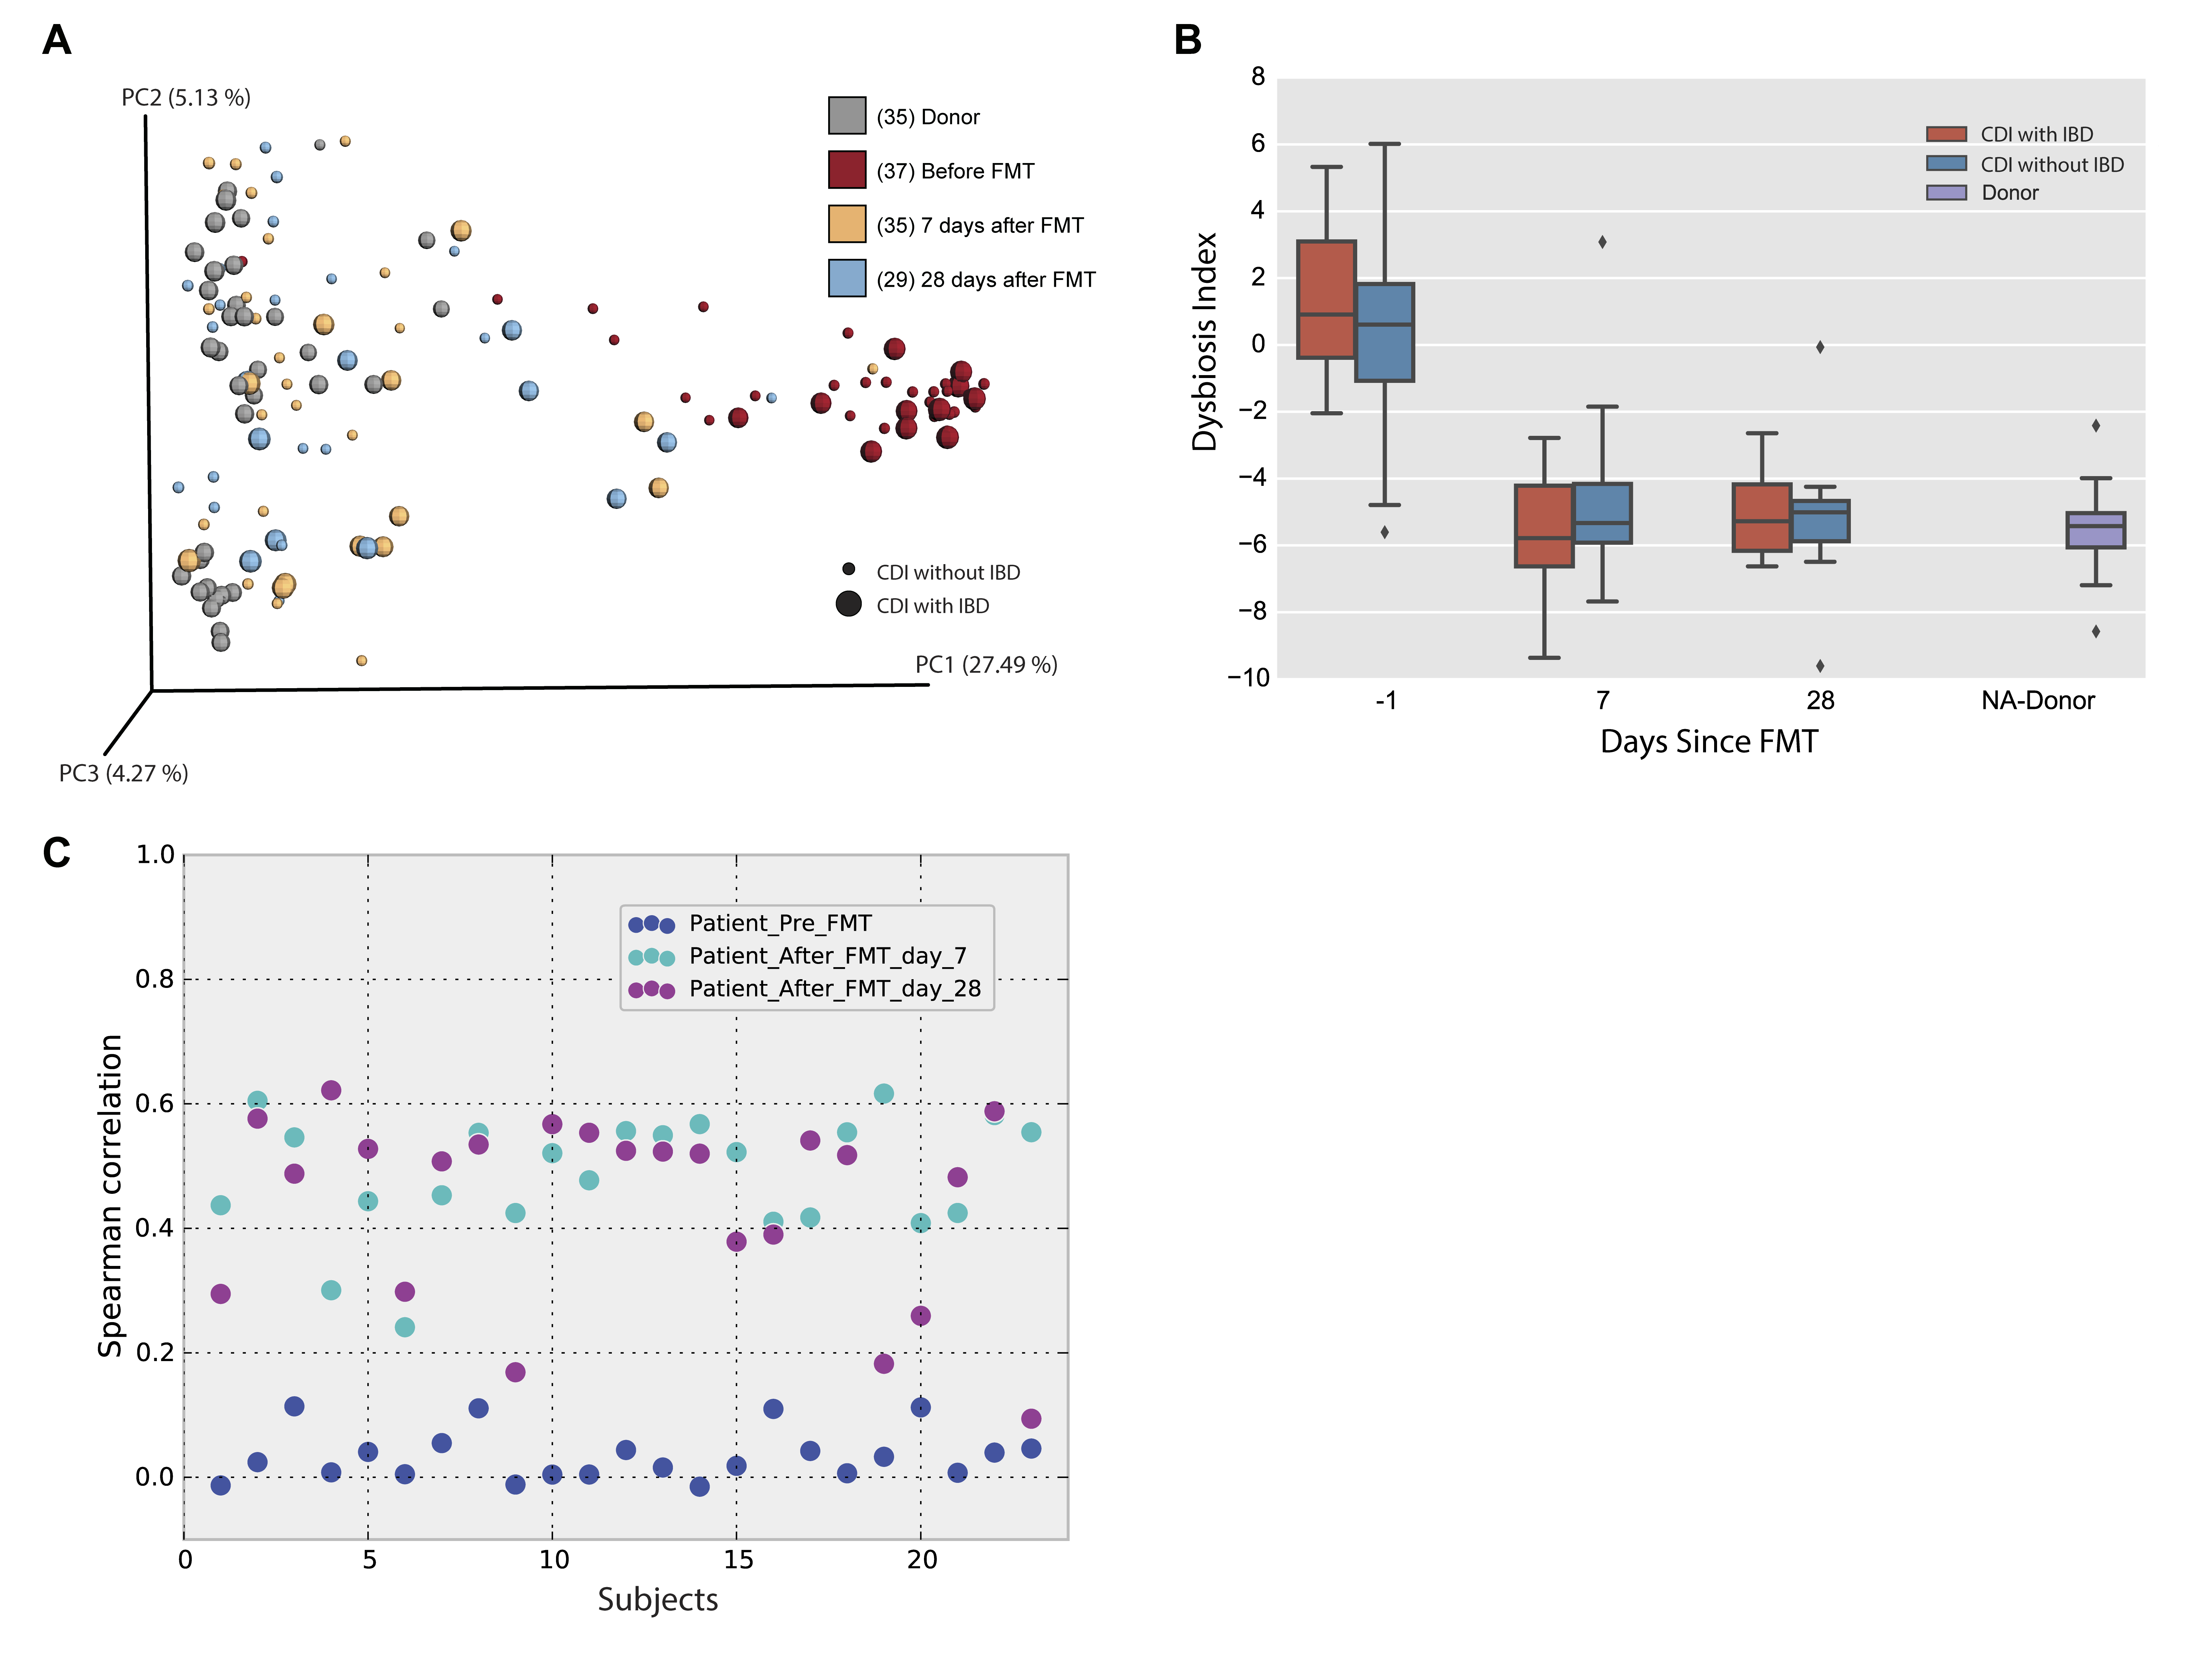
\includegraphics[width=0.8\textheight]{fmt-figures/figure-1}
\caption[Dysbiosis index and beta-diversity summaries pre- and post-fecal microbiota transplantation]{(A) Principal Coordinates Analysis of the unweighted UniFrac distances, showing change in the phylogenetic diversity between patients with CDI, 7 and 28 days after fecal microbiota transplant. (B) Change in dysbiosis index following fecal microbiota transplant in patients with CDI with or without IBD. (C) Spearman correlation to donor stool 7 and 28 days following fecal microbiota transplantation.}
\label{fmt-fig1}
\end{sidewaysfigure}

To characterize the changes in community composition, we use the \gls{md} index as a reference to describe the dominance of individual taxa (Supplementary Table 3). The \glspl{md} index is composed of 18 taxonomic groups, as defined by Gevers et al, with a higher value correlated with greater disease severity in \gls{ibd}, and lower values associated with healthier states \cite{RN1489}. As \gls{cdi} is also associated with dysbiosis and inflammation, we wanted to determine the effect of \gls{fmt} on dysbiosis. The \glspl{md} index values were significantly higher in patients with \gls{cdi} compared to donors (Mann-Whittney's U, p $<$ 0.05, Figure~\ref{fmt-fig1}B). However, on day 7 and 28 after the transplantation, the \glspl{md} index values were similar to donors (Mann-Whitney's U p $>$ 0.05, Figure~\ref{fmt-fig1}B) and this change was independent of whether recipients had \gls{ibd} or not. 

In order to determine if the changes seen in our subjects following \gls{fmt} were similar to other published studies we compared our samples with recently published data from Weingarden et al. 2015 (Supplementary Figure 2A) wherein 4 patients with \gls{rcdi} (but not \gls{ibd}) received \gls{fmt} from a single donor \cite{RN1471}. Similar to our findings, there was a rapid and sustained change in beta diversity (Supplementary Figure 2A) following \gls{fmt} and the regression to the donor plane (change in microbial composition to resemble healthy donors) following \gls{fmt} was remarkably similar in the two studies (Supplementary Figure 2B). In this context, we refer to the donor plane as a proxy to the region in the\gls{pcoa}: a dimensionality reduction method to visualize beta-diversity distance matrices) space where the donors are located; we do this by fitting a three-dimensional plane (using the least squares method) to the samples from the donors. As the communities change post-\gls{fmt}, the distance to this plane is reduced.

\subsubsection{Clinical response of CDI to FMT is independent of engraftment or donor type but underlying IBD influences changes in gut microbial ecology after FMT}

In order to determine if the response of \gls{cdi} to \gls{fmt} was dependent on donor stool engraftment, we determined Spearman's correlation coefficient between fecal microbial communities prior to and 7 and 28 days post-transplant. The fecal microbial communities from patients with \gls{cdi} were distinct from donor communities prior to transplant (Spearman's r$<$0.2 for all subjects, Figure~\ref{fmt-fig1}C). Following transplant the communities showed an increase in correlation to donor stool at day 7 (Spearman's r$>$0.4 for 85\% of the subjects, Figure~\ref{fmt-fig1}C) and a spread for all subjects at day 28 ranging from below 0.2 up to 0.6 (Figure~\ref{fmt-fig1}C). Using SourceTracker \cite{RN3995}, we found that after \gls{fmt}, subjects with \gls{ibd} retained a higher proportion of their original communities (Mann-Whitney p $<$ 0.05 at day 7, and p = 0.06 at day 28; Figure~\ref{fmt-fig2}A and \ref{fmt-fig2}B) and a significantly lower proportion of new communities (Mann-Whitney p $<$ 0.05 at day 7 and 28), as compared to the patients without \gls{ibd}. The expansion of new taxa following \gls{fmt} represents a beneficial ecological change following \gls{fmt} as seen in patients without \gls{ibd}, while those with \gls{ibd} are more prone to revert to the original community structure. Consequently, in patients with \gls{ibd} we observed a smaller group of taxa that change significantly seven days after \gls{fmt}. In both groups, \textit{Bacteroides}, and \textit{Faecalibacterium} showed a significant increase in relative abundance, with \textit{Blautia}, only being increased for patients without \gls{ibd}. Additionally, these patients showed a decrease in relative abundance of \textit{Lactobacillus}, \textit{Veillonella}, \textit{Enterobacter}, \textit{Klebsiella}, \textit{Erwina}, \textit{Proteus}, \textit{Salmonella}, and \textit{Trabulsiella} (Figure~\ref{fmt-fig2}C and~\ref{fmt-fig2}D, ANCOM p $<$ 0.05, corrected for multiple comparisons using Bonferroni-Holm's method \cite{RN1513}).

\begin{figure}[htbp]
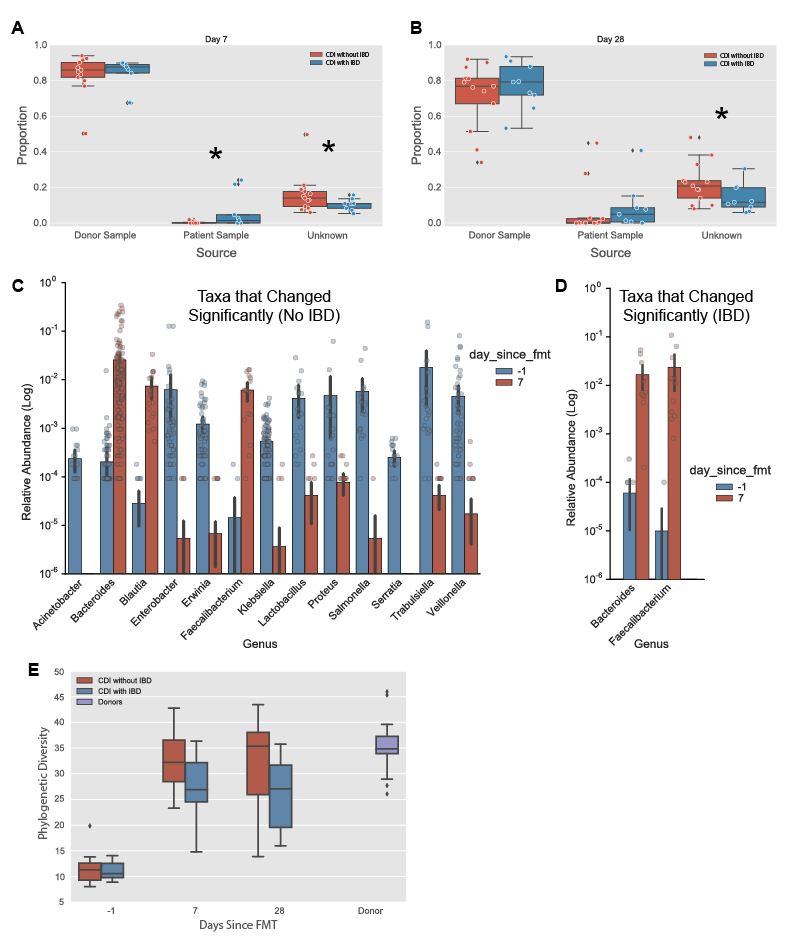
\includegraphics[width=0.95\columnwidth]{fmt-figures/figure-2}
\caption[SourceTracker and differential abundance comparison between IBD and non-IBD affected subjects.]{(A) and (B) Subjects with IBD retain a higher proportion of their original communities (Mann-Whitney p $<$ 0.05 at day 7, and p = 0.06 at day 28 and a significantly lower proportion of new communities (Mann-Whitney p $<$ 0.05 at day 7 and 28), as compared to the patients without IBD using SourceTracker. (C) Bacterial taxa that change significantly in patients with IBD after FMT (ANCOM p $<$ 0.05, corrected for multiple comparisons using Bonferroni-Holm's method). (D) Bacterial taxa that change significantly in patients without IBD after FMT (ANCOM p $<$ 0.05, corrected for multiple comparisons using Bonferroni-Holm's method). (E) Change in phylogenetic diversity based alpha diversity 7 and 28 days following fecal microbiota transplant in patients with CDI with and without IBD (Mann-Whitney's U p $<$ 0.001). }
\label{fmt-fig2}
\end{figure}

All patients had either clinical or microbiological remission, confirming that initial response of \gls{cdi} to \gls{fmt} is not dependent on the degree of donor stool engraftment. In this small cohort of patients, those with underlying \gls{ibd} had higher number of late relapses of \gls{cdi}. We found no significant differences in gut microbiota composition following \gls{fmt} from standard donors or related donors (Mann-Whitney p$>$ 0.05 at day 7 and 28), suggesting that engraftment of donor stool was independent of donor type. Furthermore as all patients had ongoing clinical remission with microbiological response (if measured), donor type does not appear to affect \gls{cdi} related clinical response.

\subsubsection{Change in bacterial diversity after FMT is dependent on underlying IBD.}

\gls{ibd} disease course, as measured by the need for specific \gls{ibd} therapies, did not change after \gls{fmt}, and patients with \gls{cdi} and underlying \gls{ibd} retained a higher proportion of the pre-transplant communities and lower proportion of new communities following \gls{fmt}.  Thus, underlying \gls{ibd} appears to affect the change in gut microbial ecology resulting in a less significant increase in overall diversity. In subjects without \gls{ibd}, Faith's phylogenetic diversity (which measures the total branch length of a phylogenetic tree that a given sample covers \cite{RN1490}) reached a level comparable to healthy donors (Mann-Whitney's U p < 0.001, Figure 2E). The differences in phylogenetic diversity following \gls{fmt} between subjects with and without \gls{ibd} became evident on day 7 and persisted on day 28 (Mann-Whitney, day -1 p = 0.163, day 7 p = 0.0058, and day 27 p = 0.008, Figure 2E). A linear regression of phylogenetic diversity vs \glspl{md} index (Supplementary Figure 3) shows a significantly lower negative correlation between the increase in phylogenetic diversity and the increase of the \glspl{md} index in patients with \gls{ibd} (Pearson's correlation coefficient, \gls{ibd} R=-0.68, No \gls{ibd} R=-0.83; p $<$ 0.0001; Supplementary Figure 3) suggesting a lack of recovery of phylogenetic diversity in patients with \gls{ibd} as the \glspl{md} index improves.

\subsection{Discussion}
In this study, we found that gut microbiota diversity changes rapidly following \gls{fmt} for treatment of \gls{cdi} and resembles donor microbiota diversity, similar to previous studies. A successful response of \gls{cdi} to \gls{fmt} was seen with a diverse group of donors and at levels of engraftment (as measured by correlation to donor stool) varying from 50-94\% (at day 7) and 34-93\% (at day 28) based on the proportion of communities attributed to the donor following \gls{fmt} per SourceTracker, suggesting these are not critical factors in determining response.  Similarly, a recent study that evaluated pre- and post-\gls{fmt} (for recurrent \gls{cdi}) gut microbiome samples from a subset of patients enrolled in a randomized controlled trial \cite{RN1527}, compared donor \gls{fmt} to autologous \gls{fmt} suggested that complete engraftment of donor bacteria may be not necessary, if functionally critical taxa are present in subjects following initial antibiotic therapy for \gls{cdi} \cite{RN1524}. This study excluded patients with \gls{ibd} but was able to compare autologous to donor \gls{fmt} unlike our study. There was a higher number of \gls{rcdi} following \gls{fmt} in patients with \gls{cdi} and \gls{ibd} but this was not statistically significant, likely given the small sample size. However we have previously reported similar findings in a larger cohort of patients with \gls{cdi} and \gls{ibd} \cite{RN1498}, where gut microbiota changes were not monitored. Interestingly, in this cohort all patients had an initial clinical or microbiological remission of \gls{cdi} following \gls{fmt} and we did not see a difference in initial response reported in a recent study \cite{RN1497}, which is also likely due to the smaller sample size of our study and differences in underlying disease characteristics. 

We also did not see changes in need for \gls{ibd} therapy in the subset of patients with \gls{ibd} underlying \gls{cdi}. While dynamic variations can be seen in patients following \gls{fmt} \cite{RN1471}, patients with underlying \gls{ibd} in our study show a higher proportion of the original pre-transplant microbial community and lower recovery of phylogenetic diversity following \gls{fmt} compared to those without \gls{ibd}. This lack of beneficial change in microbial ecology may be relevant for long term response of \gls{cdi} in patients with \gls{ibd} and the lack of clinical response of \gls{ibd} to \gls{fmt} seen in our and previous studies \cite{RN1497}. Future studies designed to study the effect of compositional and functional changes in gut microbiota on clinical outcomes following \gls{fmt} in patients with \gls{ibd} will be needed to definitively address the potential importance of changes in microbial ecology, donor selection \cite{RN3982}, underlying disease characteristics and multiple-dose \glspl{fmt}, in correcting the underlying pathophysiology of \gls{ibd}. 

\subsection{Conclusions}

There is a significant increase in microbial diversity in patients with recurrent \gls{cdi} after \gls{fmt}. Both, the degree of microbial engraftment or donor type (related or unrelated) are not key for successful treatment of \gls{rcdi} by \gls{fmt}. Compared to \gls{cdi} patients without \gls{ibd}, \gls{cdi} patients with \gls{ibd} have higher proportion of the original microbial communities after \gls{fmt} and increased episodes of future \gls{cdi} on long-term follow-up.

\else
    \section{FMT paper 1}\label{section_moviefmt}
    \section{FMT paper 2}\label{section_fmt}
\fi

\chapter{Future Work}

\url{https://ptpb.pw/b7_V.png}

This thesis presents a collection of static and dynamic snapshots of diverse
microbial systems. Although our new methods are in no way specific to the human
gut, part of our focus has been to bridge the gap between computation and
biology, to get us closer towards a future where drug prescription, diet and
recreational activities can be further \textit{personalized} -- through a layer
invisible to the naked eye but perceivable in most respects of life.

It seems impossible to accurately predict the impact of scientific discoveries, 
historically, we have seen great evidence of seemingly anachronistic findings 
(for example neural networks \cite{Tem10}) that later, usually when other 
technologies catch up, become new fields of research or cornerstones in 
consumer applications.  Therefore, while acknowledging this is a tough problem, 
I present my personal view on future directions that can build up from the 
contributions in this thesis. I divide these into three sections: diagnostic 
methods, treatment and analysis.

\section{Diagnostic Methods}

In Chapter~\ref{chapter_dogs} and Chapter~\ref{chapter_ibds}, we presented
examples of biomarkers for \gls{ibd} and \gls{cd} from two different analytical 
perspectives.  First, in a dog cohort, we showed that we can reformulate the 
dysbiosis index we originally developed for humans \cite{Gevers2014}, and make 
it specific for a different host\hyp{}species. Both in humans and dogs, this 
log-ratio of bacterial groups is associated with decreased phylogenetic 
diversity, and in humans, it is also associated with inflammation.  Next, after 
noticing the increased volatility in the microbiome of subjects with \gls{ibd}, 
we benchmarked microbial variability in fecal samples as an effective 
classifier for disease.  This method is powerful, because it overcomes the low 
classification accuracy of fecal samples, and improves as more samples per 
subject are collected.

Although both approaches are encouraging, translating research into 
consumer\hyp{}level applications, commonly presents formidable challenges that 
might only be solvable by future generations.  Take for example the \gls{ecg}, 
it took almost 125 years, between the first observation of 
biopotentials\footnote{Credited to Luigi Galvani in 1787.}, and the moment when 
the first table \gls{ecg}\footnote{Willem Einthoven's ectrocardiograph was 
manufactured by the Cambridge Scientific Instrument Company of London in 1911.} 
became commercially available \cite{ECGZywietz}. Even after the tremendous 
progress, proper validation of computer-generated diagnostics only appeared 
more than 200 years after the initial discovery \cite{njem_ecg}.

I use the example of the \gls{ecg}, because much like raw heart biopotentials,
(\textit{i}) microbiome data is plagued with noise, and (\textit{ii})
determining the appropriate filters and thresholds directly depends on the
use-case. However, unlike with the early developments of the \gls{ecg}, we live
in digital and connected world. As such, the following focuses will
shorten the time between future discoveries and innovation:

\begin{description}
    \item[Mechanistic Studies]The novelty characteristic of microbiome studies, 
        has produced a large amount of descriptive studies, contrastingly, 
        mechanistic experiments have lagged in validating several of these 
        findings (likely due to the more expensive requirements).  If the goal 
        is to relate the presence or abundance of a microbiome feature to a
        disease state or biochemical process, the underlying methods must be 
        informed by biological inferences in order for these biomarkers to gain 
        credibility.

    \item[Open Data]Medical research is specially affected by human factors, 
        being able to consistently collect samples from a subject is not always 
        easy or deterministic (think of bowel problems and fecal samples). A 
        powerful practice used to counter underpowered studies, is to improve 
        on the current sample size through the reuse of previously published 
        data. This approach is only possible through open resources like 
        Qiita\footnote{\url{https://qiita.ucsd.edu/}}, makes data reuse 
        seamless. Importantly, the work in this thesis was only possible 
        through the reuse of existing datasets (see 
        Chapter~\ref{exploratory_chapter} through Chapter~\ref{chapter_fmts}).  
        Although making data openly available is an important first step, 
        proper standardization of processing protocols, will also be key to 
        maximizes data re-usability, a remarkable example of this practice is 
        the \gls{emp} \cite{RN4267}.
\end{description}

\section{Treatment}

Microbiome\hyp{}based treatments, are generally based on the transplantation of 
microbial communities from a \textit{healthy} donor into an affected 
\textit{recipient}. Three spearheading examples are: \glspl{fmt} to treat 
\gls{cdi} \cite{RN4129}, skin microbiomes transplants to treat atopic 
dermatitis \cite{GalloSkin}, and (although still in early stages) a capsule 
full of microbial spores to treat \gls{uc} by Seres 
Therapeutics\footnote{\url{http://www.serestherapeutics.com}}.

Although most \glspl{fmt} succeed at treating \gls{cdi}, what makes a
successful transplant is not clear yet, the number of variables implicated in
answering this question is immense. From a computational complexity standpoint,
\textit{a priori} determination of whether or not a new community can colonize 
an existing ecosystem is considered a hard problem, belonging to the 
\textbf{\#-P} class \cite{RN4266}. As such our focus should be on strengthening 
our systematic understanding of the transplant, and characterize not only what 
makes a successful transplant but also what makes a failed one.  For example, 
the impact of the work presented in Section~\ref{section_fmt} could have been 
magnified, if we had included subjects for which the \gls{fmt} failed. With 
appropriate sample sizes, we could have applied a number of techniques to 
single out (if any) the features common that lead to a failed transplant. With 
this knowledge, we could pre-screen \textit{donors} and \textit{recipients} to 
ensure a successful treatment.

\section{Analysis}

Much like our microbial symbionts depend on the host environment (and vice
versa), the development and funding of analytical tools depends on the
ever-growing necessity to unravel complex patterns in a number of experimental
setups (cross-sectional, longitudinal, multi-'omic, etc). Thus, these tools,
must take into consideration the ability to be flexible, scalable and when
possible interactive.

Novel analytical methods and software infrastructure, should be built making 
scalability a priority.  We have seen a steady increase in our capability to 
generate data, and it is likely that this trend will continue. Emperor 
(Chapter~\ref{chapter_emperor}) was partly a response to the limitations in 
existing software, and more recently we had to re-architect the underlying 
implementation to cope with modern and larger datasets.

Flexibility and compliance with community standards, makes software available
to a wider audience. Take the count table, often acting as the core
data-structure for metabolomic, transcriptomic, proteomic, (and other 'omics)
analyses. If the software producing this data complies with a standard, like
the \gls{biom}-format, the end user is now free to select from a variety of
methods as opposed to being limited to nieche-software. This idea is being
taken a step further with \gls{qiime} 2, where a semantic type system defines
the methods and visualizations that can be applied to any given dataset.

Finally, the value of interactively exploring a dataset, lies on our ability to
quickly test hypotheses, and iteratively develop new ones. Future exploratory
analysis tools should be developed with interoperability in mind, for example,
brushing to select a group of samples in a view of data might act as a filter
for a different representation. Modern web technologies, and software
development frameworks like \gls{qiime}2 will likely be the pioneers of these
global overviews of microbial diversity.


\appendix
\chapter{Sample collection and processing for 
Chapter~\ref{chapter_dogs}}\label{appendix_dogs}

\section{Methods}

Naturally passed fecal samples were analyzed from 85 healthy dogs and 65 dogs 
with chronic signs of gastrointestinal disease and confirmed inflammatory 
changes on histopathology. All dogs participated in different clinical studies 
and leftover fecal samples were utilized for this study. The protocol for 
sample collection was approved by the Clinical Research Review Committee of the 
College of Veterinary Medicine, Texas A\&M University (CRRC\#09-06). 

Dogs with clinical signs of chronic \gls{gi} disease (i.e., vomiting, diarrhea, 
anorexia, weight loss, etc.) were diagnosed with idiopathic \gls{ibd} based on 
the\gls{wsava} criteria: (i) chronic (i.e., $>$ 3 weeks) GI signs; (ii) 
histopathologic evidence of mucosal inflammation; (iii) inability to document 
other causes of GI inflammation; (iv) inadequate response to dietary, 
antibiotic, and anthelmintic therapies, and (v) clinical response to 
anti-inflammatory or immunosuppressive agents.  Histological samples were 
obtained endoscopically. The clinical status of each dog was evaluated using a 
published clinical \gls{cibdai}. Within the \gls{ibd} dogs, 41 dogs had 
histological confirmed inflammation in the small intestine, 18 dogs had 
histological changes in both small intestine and colon, and 5 dogs had only 
histological changes reported in the colon. Histological changes were 
predominantly of lymphoplasmacytic infiltrates, with a subset of dogs also 
showing eosinophilic and/or neutrophilic components. The mean (SD) \gls{cibdai} 
for \gls{ibd} dogs was 6.4 (3.1).

Dogs were excluded if they received antibiotics within the past 2 weeks of 
sample collection. Data on antibiotic history was nevertheless collected: 34/65 
dogs with \gls{ibd} had no history of prior antibiotics administration, while 
13 dogs received antibiotics several weeks ($>$2) or months before sample 
collection. The remaining 18 dogs in the \gls{ibd} group had no information 
about prior antibiotic use. In the healthy group (n=85), 76 dogs had not 
received any antibiotics, and 9 dogs had a history of antibiotic use, but not 
within the last 2 weeks of sample collection. No technical replicates were 
generated in this study.

Sample and animal information (i.e., age, weight, gender, breed, duration of 
clinical signs, histopathology, antibiotic usage) was obtained from clinical 
records. Also, if the owner provided the information, the exact diet (trade 
name and manufacturer) fed at time of sample collection was recorded in the 
clinical records, and the dietary macronutrients (protein, fat, and 
carbohydrate content) were recorded from manufacturer's provided data on the 
labels.

Body weights ranged from 2.9 to 55 kg (mean 22 kg, SD: 14.9 kg), which was not 
significantly different from (Mann Whitney test; p=0.087) the healthy dogs 
(range 0.9 to 50 kg; mean 20.3 kg, SD: 10.7g). Mean age (SD) was 5.4 (3.07) in 
the \gls{ibd} group, which was not significantly (Mann Whitney test; p=0.311) 
different from healthy dogs (4.7, 3.2). There was a wide breed distribution 
with 37 different breeds in the \gls{ibd} group and 42 different breeds in the 
control group. In the \gls{ibd} group, Yorkshire terrier, German Shepherd dogs 
and Labrador Retrievers (n=5 each) were most commonly represented.

\Gls{bcs} were assessed according to the \gls{wsava} criteria. \Gls{bcs} is 
rated in a 9-point scale that visually evaluates a dog's body composition. This 
score has been validated against the standard \gls{dexa} \cite{RN4000}. For 
this dataset, the \Gls{bcs} was restricted to a subset of the healthy samples, 
therefore \gls{ibd} vs. Healthy comparisons could not be made in this case.

\subsection{DNA Extraction and Sequencing}

DNA isolation was performed as described by the \gls{emp} Protocol (version 
4\textunderscore 13) for 16S rRNA\cite{RN164}. The full cohort included 192 
samples, of which 15 were removed because those subjects had acute hemorrhagic 
diarrhea, and had little clinical information available.  The remaining 28 
samples did not recover enough sequences after quality control including 
screening for low counts of reads per sample. All samples were sequenced using 
the Illumina HiSeq platform (2 x 100 nucleotide sequences and an index read).

\subsection{Accession Numbers}

Raw sequences for the dog samples have been deposited to the \gls{ena} at the 
following accession number ERP014919, equivalent processed \gls{otu} tables and 
metadata can be accessed through 
Qiita\footnote{\label{qiitaurl}\url{https://qiita.microbio.me}} under study 833 
- `Dog models of inflammatory bowel disease'.

The data for the human dataset\cite{RN154} can be found in the \gls{ena} at the 
following accession numbers ERP015241 and ERP015242, equivalent processed 
\gls{otu} tables and metadata can be accessed through 
Qiita\textsuperscript{\ref{qiitaurl}} under study identifiers 1939 and 1998 
-`The Treatment-Naive Microbiome in New-Onset Crohn's Disease'.

Data for the additional dog study \cite{RN153} can be found at the \gls{sra} of 
the under accession number SRP040310.

\chapter{Sample collection and processing for 
Chapter~\ref{chapter_ibds}}\label{appendix_ibds}

\section{Methods for Section~\ref{section_plane}}\label{appendix_plane}

\subsection{Cohort Demographics}

Patients with \gls{cd} or \gls{uc}, the two major forms of \gls{ibd}, attending 
the outpatient clinic were consecutively invited to take part. After obtaining 
written consent, \gls{bmi} was recorded and patients were asked to provide a 
fecal sample and to fill in a questionnaire with clinical disease activity, 
present medication, dietary habits, use of antibiotics and use of 
\glspl{nsaid}. Disease phenotype was classified according to the Montreal 
classification \cite{Silverberg2005}. Individuals were then followed 
prospectively, asked to provide fecal samples and to fill in the questionnaire 
every third month for a two-year period. If a patient did not provide a fecal 
sample at any of the three months periods, a reminder letter was sent. In total 
109 patients with \gls{ibd} (\gls{cd}; n=49 and \gls{uc}; n=60) took part. Nine 
additional individuals with no \gls{ibd} or any other gastrointestinal 
conditions were recruited as \gls{hc} as well as 19 patients with other chronic 
inflammatory gastrointestinal diseases (4 \gls{lc} and 15 \gls{cc}).  All 137 
individuals were Caucasians and together they provided 683 fecal samples during 
the two-year period (Supplementary 
Table~4\footnote{\url{https://images.nature.com/original/nature-assets/nmicrobiol/2017/nmicrobiol20174/extref/nmicrobiol20174-s1.pdf}}).  
The study was approved by the Ethical Committee of the Medical Faculty, Uppsala 
University (2007/291).

\subsection{Sample Collection}

Fecal samples were self-collected in sterile plastic containers and stored at 
-80 °C until shipping on dry ice and processing.

\subsection{Fecal calprotectin} 

To assess the degree of inflammatory activity at the collection of each fecal 
sample, the concentration of f-calprotectin was assessed by commercially 
available ELISA, Calprotectin Elisa Buhlmann Laboratories AG, Basel, 
Switzerland, according to the manufacturer's protocol. 

\subsection{DNA Extraction and Amplification}

Genomic DNA was extracted from 0.25 g of fecal material from each sample using 
the Earth Microbiome DNA extraction protocol \cite{EMP2011}. Briefly, DNA was 
extracted using the 96-well format MoBio Powersoil DNA kit on an EpMotion 5075 
robot with vacuum (Eppendorf, Hamburg, Germany). DNA was quantified with the 
Qubit 2.0 fluorometer (Invitrogen, Carlsbad, CA) according to the 
manufacturer's instructions.

PCR amplification and library preparation were performed similarly to the 
protocol described by Caporaso et al. \cite{Caporaso2011proceedings}. 515F/806R 
Illumina primers with unique reverse primer barcodes were used to target the V4 
region of the 16S rRNA gene. Samples were amplified in triplicate and cleaned 
using the MO BIO 69 htp PCR cleanup kit. Each PCR reaction included 1X PCR 
buffer, 10 $\mu$M each forward and reverse primer, 200 μM dNTPs, 1 U/ml Taq 
polymerase, 15 ng template DNA, and PCR grade water, with a total reaction 
volume of 25 $\mu$L. Reactions were kept at 94\textdegree C for 3 minutes for 
denaturation to occur. Amplification was performed by 25 cycles of 
94\textdegree C for 45s, 58\textdegree C for 60s, and 72\textdegree C for 90s.  
The V4 amplicons were sequenced on the Illumina HiSeq 2000 platform, yielding 
single end, 100 base pair reads. Sequencing and quality assessment were 
performed at the Yale Center for Genome Analysis.

\subsection{Data Availability}

Microbiome data from this study is available on Qiita under study ID 1629 
(https://qiita.ucsd.edu/study/description/1629) and using the EBI accession 
number ERP020401. Patient clinical information is available on Qiita and in 
Supplemental 
Dataset~1\footnote{\url{https://images.nature.com/original/nature-assets/nmicrobiol/2017/nmicrobiol20174/extref/nmicrobiol20174-s2.txt}}. 

\section{Methods for Section~\ref{section_ibd}}\label{appendix_ibd}

\subsection{Fecal collection}

Stool was collected daily using a swab technique \cite{RN4220}, which enables 
the study subject to collect stool samples from the toilet paper. Samples were 
stored on a -20\textdegree C freezer. Fifteen patients collected daily stool 
for two 2-week periods separated by an interval of 4 weeks, during which no 
stool was collected.  The short \gls{cdai} was evaluated at entry and at 
the end of collection period 1 and 2 \cite{RN4006}. The collection periods 
for the family substudy, which included 4 patients with inactive \gls{cd} 
with same exclusion criteria as above and 3 unaffected family members of 
each \gls{cd} patient were two separate 4 weeks periods interrupted by a 3 
month collection-free interval.

Patients with proven \gls{cd} diagnosed for at least 3 months and in clinical 
remission were recruited at the University of North Carolina (see 
Table~\ref{ibd-table1}). Serial stool samples as outlined below were submitted 
for analysis. Exclusion criteria for entry into the study were active \gls{cd} 
as defined by a short \gls{cdai} score $>$ 150; fistulizing \gls{cd}, 
concomitant use of azathioprine (AZA), 6-mercaptopurine (6-MP), methotrexate or 
anti-TNF agents for less than 3 months; or concomitant use of systemic steroids 
or budesonide. Steroids or budesonide had to be discontinued at least 8 weeks 
before inclusion, and local, rectally administered therapies containing 5-ASA 
(enemas, suppositories) or steroid enemas/foams should have not been used for 
the previous 4 weeks. Also, \glspl{nsaid} were not allowed as regular 
treatment, which was defined as use for at least 4 days a week each month.  
Patients were excluded if they were on antibiotic therapy $\geq$5 days each 
month or had antibiotic therapy $\geq$5 days in the previous 24 weeks. No 
probiotics were allowed in the last 24 weeks before inclusion and patients on 
long-term therapy with narcotics $>$2 days weekly were excluded.  Further 
subject exclusions were known Hepatitis B, Hepatitis C or PSC or regular, high 
dose alcohol consumption (more than seven drinks per week). All trial 
participants were prohibited from consuming specific diets (e.g. Atkins diet, 
low carbohydrate diet). In the second subset we also included nonaffected 
family members to collect serial fecal samples.  The requirement for the family 
subjects was one sibling age $\geq$ 8 years without known \gls{cd} or 
ulcerative colitis and two living parents without \gls{cd} or ulcerative 
colitis. The same exclusion criteria for antibiotics, probiotics, narcotics and 
concomitant diseases as in the main study were applied. 

\begin{table}[htbp]
    \centering
    \caption{Summary of the demographic data of the 19 CD patients.}
    \label{id-tabMethods}
    \begin{tabular}{rrl}
    \toprule
         \multicolumn{2}{r}{Male/Female (n)} &	8 / 11\\
    \midrule
    \multicolumn{2}{r}{Age (years, median; range)} &	31 (15-51)\\
\midrule
\multicolumn{2}{r}{Duration of Crohn's disease (years median; range)} &	9 (0.5-35)\\
\midrule
\multirow{3}{*}{Location of Crohn's disease (n)} & 	Ileal & 5\\
 &   	Ileo-colonic & 10\\
 &     	Colonic	 & 4\\
\midrule
\multicolumn{2}{r}{History of ileocecal resection} &	7\\
\midrule
\multicolumn{2}{r}{History of isolated small intestinal resection} &	2\\
\midrule
\multirow{4}{*}{Concomitant therapies (n)} &        	Steroids & 0\\
&        	Azathioprine/6-MP/methotrexate & 8\\
 &        	anti-TNF agent & 12\\
     &   	5-ASA	 &2\\
\midrule
\multicolumn{2}{r}{\gls{cdai} end of week 2 (mean; SD)} &	63 (51)\\
\midrule
\multicolumn{2}{r}{\gls{cdai} end of week 4 (mean; SD)} &	72 (61)\\
\bottomrule
    \end{tabular}
\end{table}

\subsection{DNA Extraction}

Fecal DNA isolation was performed according to the 16S Earth Microbiome Project 
Protocol \cite{RN164}. Of the 960 samples analyzed, the initial subset (384 
samples)  were processed using the Illumina MiSeq platform (150 nucleotide 
sequences), and for the second subset (576 samples) were processed using the 
HiSeq platform (100 nucleotide sequences).

\subsection{Data Availability}

The sequences have been deposited on EBI and are available under the following
accession number ERP104742.  In addition, the processed sequences and sample
information can be found in the
Qiita\footnote{\url{https://qiita.ucsd.edu/study/description/2538}} database
under the study identifier 2538.

\chapter{Sample collection and processing for 
Chapter~\ref{chapter_fmts}}\label{appendix_fmts}

\section{Methods for Section~\ref{section_moviefmt}}\label{appendix_moviefmt}

\subsection{Patients and donors}
All patients suffered from multiply \gls{rcdi} refractory to standard 
antibiotic therapies. A single standard donor was used in the preparation of 
all fecal microbiota material as described previously \cite{RN45}. The 
Institutional Review Board at the University of Minnesota approved prospective 
collection of fecal specimens and their analysis. All patients satisfied the 
inclusion criteria for the \gls{fmt} within our program, which included at 
least two spontaneous recurrences of \gls{cdi} within a month of 
discontinuation of antibiotics and failure of at least one advanced antibiotic 
regimen such as a vancomycin pulse/taper protocol or vancomycin treatment 
followed by administration of rifaximin or fidaxomicin for 2-3 weeks.  The 
specific clinical characteristics of patients involved in this study are 
summarized in Supplementary 
Table~1\footnote{\url{https://static-content.springer.com/esm/art\%3A10.1186\%2Fs40168-015-0070-0/MediaObjects/40168_2015_70_MOESM3_ESM.xlsx}}.  

\subsection{Fecal microbiota transplantation}
\Gls{fmt} was done using a standardized preparation of concentrated fresh or 
frozen fecal bacteria via colonoscopy as previously described \cite{RN45}. All 
patents were treated with oral vancomycin, 125 mg four times daily, until two 
days prior to the procedure \cite{RN45}. The day before the procedure, patients 
received a polyethylene glycol-based colonoscopy prep 
(GoLYTELY\textsuperscript{\textregistered} or 
MoviPrep\textsuperscript{\textregistered}) to remove residual antibiotics and 
fecal material. Donor fecal microbiota was placed into the terminal ileum 
and/or cecum via the biopsy channel of the colonoscope. A total of 17 donor 
samples from the same individual were used in these studies.  The CD1-CD4 donor 
samples were given to patients CD1-CD4, respectively. Patients CD1, CD3, and 
CD4 received freshly prepared fecal microbiota, while patient CD2 received a 
previously frozen preparation of fecal microbiota, all from the same 
standardized, anonymous donor.

\subsection{Sample collection}
Fecal samples were collected at home by the patients using swabs to sample 
feces deposited into a toilet hat immediately after production, and stored 
frozen at approximately -20\textdegree C. Samples were subsequently transferred 
to the laboratory and stored at -80\textdegree C until used. Donor samples for 
DNA extraction were collected during processing of material for \gls{fmt}, and 
stored frozen at       -80\textdegree C until used. Samples from patients CD1- 
4 were obtained prior to \gls{fmt} and between 1 to 151 days post-\gls{fmt}, 
with daily collection until day 28, and weekly collection until day 84. Fecal 
material prior to \gls{fmt} was obtained from patients CD5-CD14.

\subsection{DNA extraction}
DNA was extracted from donor and recipients' pre- and post-\gls{fmt} fecal 
samples using MOBIO PowerSoil DNA extraction kits (MOBIO, Carlsbad, CA), 
according to the manufacturer's instructions. Fecal DNA concentrations were 
measured using a QuBit DNA quantification system (Invitrogen, Carlsbad, CA).

\subsection{PCR amplification}
Extracted DNA was amplified using the EMP standard 
protocols\footnote{\url{http://www.earthmicrobiome.org/}} following the 
recommendations of Caporaso et al. \cite{RN4221}. Briefly, F515/R806 primers 
were used, with 12-base Golay codes introduced on the 806 end to provide unique 
sample indices. Cycling and annealing conditions were as previously described 
\cite{RN4221}.

\subsection{DNA sequencing}
DNA sequencing was performed as previously described \cite{RN4221} on an 
Illumina MiSeq platform using 2 x 150 bp paired-end reads and the Illumina v3 
reagent chemistry. 

\section{Methods for Section~\ref{section_fmt}}\label{appendix_fmt}

\subsection{Patient selection}

Patients undergoing \gls{fmt} for \gls{rcdi} were prospectively recruited in 
this study. Informed consent was obtained to collect clinical data and stool 
samples. Data collected included demographics, clinical history, \gls{cdi} 
treatment history, comorbid conditions and response to \gls{fmt}. A donor fecal 
sample was collected prior to \gls{fmt}. Stool samples from the recipients were 
collected before \gls{fmt}, and at day 7 and day 28 and were stored at 
-80\textdegree C. The donors were either related (genetically related family 
members) or unrelated (screened hospital employee volunteer donors or unrelated 
family members) and a fresh sample was obtained on the day of \gls{fmt}. All 
donors underwent extensive screening in accordance with standard practice and 
guidelines from the Food and Drug Administration \cite{RN1446}. Donor selection 
criteria and experience from our group have been previously published 
\cite{RN1523}. The donor stool sample is weighed and divided into 50 grams 
aliquots. Each aliquot of 50 grams is diluted in normal saline in a 1:5 ratio 
(50 grams of stool diluted with 250 ml of normal saline) and is placed in the 
blender bag (a 2 bag system with a semipermeable membrane in the inner bag and 
the outside bag is plastic). The stool is placed in the inner bag and normal 
saline is added. The bag is placed in a sealed compartment in the stomacher 400 
(Seward) and blended for 60 seconds at 230 rotations per minute. The filtrate 
is then placed into 50 ml conical tubes using 50 ml pipettes and placed on an 
ice pack prior to the procedure.  \Gls{rcdi} was defined as another episode of 
\gls{cdi} within 56 days after symptom resolution with recurrence of symptoms 
and a positive stool polymerase chain reaction test. For this study, future 
\textit{C. difficile} episodes after \gls{fmt} up to 2 years were captured.  
These were categorized as up to 56 days, 56 days to 1 year and beyond 1 year. 

\subsection{Sequencing and analytic methods}

After fecal DNA isolation (MoBio, Carlsbad, CA fecal DNA kit), amplicons 
spanning the variable region 4 of bacterial 16S rRNA were generated and 
sequenced using Illumina MiSeq platform at the Mayo Clinic Medical Genome 
Facility, Rochester, MN. The 16S rRNA sequencing data from the Illumina runs 
were quality controlled, trimmed, demultiplexed and assigned to \glspl{otu} 
following the closed reference at 97\% similarity (using SortMeRNA as a 
clustering algorithm \cite{RN3810} protocol against the Greengenes \cite{RN165} 
database 13\textunderscore 8 release, as implemented in \gls{qiime} 1.9.0 
software \cite{RN110}, default parameters were used for all these steps unless 
otherwise noted. After quality control, 10,583,052 sequences were obtained, for 
a mean of 76,688 sequences per sample (min: 33,559, max: 154,200).


\subsection{Clinical Statistics}

Statistical analyses for clinical data were performed with JMP version 11.0 
(SAS institute, NC).  Data analysis included descriptive statistics, t-tests 
for normally distributed variables, non-parametric tests for skewed variables, 
chi-square tests and ANOVA tests as applicable. A p-value less than 0.05 was 
considered statistically significant.


%% END MATTER
\printindex %% Uncomment to display the index
% \nocite{}  %% Put any references that you want to include in the bib 
%               but haven't cited in the braces.
% \bibliographystyle{alpha}  %% This is just my personal favorite style. 
%                              There are many others.
\bibliography{references}
\bibliographystyle{plain}

\end{document}
